\documentclass[twoside]{article}

% Packages required by doxygen
\usepackage{fixltx2e}
\usepackage{calc}
\usepackage{doxygen}
\usepackage[export]{adjustbox} % also loads graphicx
\usepackage{graphicx}
\usepackage[utf8]{inputenc}
\usepackage{makeidx}
\usepackage{multicol}
\usepackage{multirow}
\PassOptionsToPackage{warn}{textcomp}
\usepackage{textcomp}
\usepackage[nointegrals]{wasysym}
\usepackage[table]{xcolor}

% Font selection
\usepackage[T1]{fontenc}
\usepackage[scaled=.90]{helvet}
\usepackage{courier}
\usepackage{amssymb}
\usepackage{sectsty}
\renewcommand{\familydefault}{\sfdefault}
\allsectionsfont{%
  \fontseries{bc}\selectfont%
  \color{darkgray}%
}
\renewcommand{\DoxyLabelFont}{%
  \fontseries{bc}\selectfont%
  \color{darkgray}%
}
\newcommand{\+}{\discretionary{\mbox{\scriptsize$\hookleftarrow$}}{}{}}

% Page & text layout
\usepackage{geometry}
\geometry{%
  a4paper,%
  top=2.5cm,%
  bottom=2.5cm,%
  left=2.5cm,%
  right=2.5cm%
}
\tolerance=750
\hfuzz=15pt
\hbadness=750
\setlength{\emergencystretch}{15pt}
\setlength{\parindent}{0cm}
\setlength{\parskip}{3ex plus 2ex minus 2ex}
\makeatletter
\renewcommand{\paragraph}{%
  \@startsection{paragraph}{4}{0ex}{-1.0ex}{1.0ex}{%
    \normalfont\normalsize\bfseries\SS@parafont%
  }%
}
\renewcommand{\subparagraph}{%
  \@startsection{subparagraph}{5}{0ex}{-1.0ex}{1.0ex}{%
    \normalfont\normalsize\bfseries\SS@subparafont%
  }%
}
\makeatother

% Headers & footers
\usepackage{fancyhdr}
\pagestyle{fancyplain}
\fancyhead[LE]{\fancyplain{}{\bfseries\thepage}}
\fancyhead[CE]{\fancyplain{}{}}
\fancyhead[RE]{\fancyplain{}{\bfseries\leftmark}}
\fancyhead[LO]{\fancyplain{}{\bfseries\rightmark}}
\fancyhead[CO]{\fancyplain{}{}}
\fancyhead[RO]{\fancyplain{}{\bfseries\thepage}}
\fancyfoot[LE]{\fancyplain{}{}}
\fancyfoot[CE]{\fancyplain{}{}}
\fancyfoot[RE]{\fancyplain{}{\bfseries\scriptsize Generated by Doxygen }}
\fancyfoot[LO]{\fancyplain{}{\bfseries\scriptsize Generated by Doxygen }}
\fancyfoot[CO]{\fancyplain{}{}}
\fancyfoot[RO]{\fancyplain{}{}}
\renewcommand{\footrulewidth}{0.4pt}
\renewcommand{\sectionmark}[1]{%
  \markright{\thesection\ #1}%
}

% Indices & bibliography
\usepackage{natbib}
\usepackage[titles]{tocloft}
\setcounter{tocdepth}{3}
\setcounter{secnumdepth}{5}
\makeindex

% Hyperlinks (required, but should be loaded last)
\usepackage{ifpdf}
\ifpdf
  \usepackage[pdftex,pagebackref=true]{hyperref}
\else
  \usepackage[ps2pdf,pagebackref=true]{hyperref}
\fi
\hypersetup{%
  colorlinks=true,%
  linkcolor=blue,%
  citecolor=blue,%
  unicode%
}

% Custom commands
\newcommand{\clearemptydoublepage}{%
  \newpage{\pagestyle{empty}\cleardoublepage}%
}

\usepackage{caption}
\captionsetup{labelsep=space,justification=centering,font={bf},singlelinecheck=off,skip=4pt,position=top}

%===== C O N T E N T S =====

\begin{document}

% Titlepage & ToC
\hypersetup{pageanchor=false,
             bookmarksnumbered=true,
             pdfencoding=unicode
            }
\pagenumbering{alph}
\begin{titlepage}
\vspace*{7cm}
\begin{center}%
{\Large Midnight Blue }\\
\vspace*{1cm}
{\large Generated by Doxygen 1.8.12}\\
\end{center}
\end{titlepage}
\pagenumbering{roman}
\tableofcontents
\pagenumbering{arabic}
\hypersetup{pageanchor=true}

%--- Begin generated contents ---
\section{Namespace Index}
\section{Namespace List}
Here is a list of all documented namespaces with brief descriptions\+:\begin{DoxyCompactList}
\item\contentsline{section}{\hyperlink{namespace_midnight_blue}{Midnight\+Blue} }{\pageref{namespace_midnight_blue}}{}
\item\contentsline{section}{\hyperlink{namespace_midnight_blue_1_1_testing}{Midnight\+Blue.\+Testing} }{\pageref{namespace_midnight_blue_1_1_testing}}{}
\end{DoxyCompactList}

\section{Hierarchical Index}
\subsection{Class Hierarchy}
This inheritance list is sorted roughly, but not completely, alphabetically\+:\begin{DoxyCompactList}
\item \contentsline{section}{M\+B2\+D.\+Collectable}{\pageref{class_m_b2_d_1_1_collectable}}{}
\item \contentsline{section}{M\+B2\+D.\+Collision.\+Collision\+Cell}{\pageref{class_m_b2_d_1_1_collision_1_1_collision_cell}}{}
\item \contentsline{section}{M\+B2\+D.\+Collision.\+Collision\+Map}{\pageref{class_m_b2_d_1_1_collision_1_1_collision_map}}{}
\item \contentsline{section}{M\+B2\+D.\+I\+O.\+Command}{\pageref{class_m_b2_d_1_1_i_o_1_1_command}}{}
\begin{DoxyCompactList}
\item \contentsline{section}{M\+B2\+D.\+I\+O.\+Console\+Command}{\pageref{class_m_b2_d_1_1_i_o_1_1_console_command}}{}
\item \contentsline{section}{M\+B2\+D.\+I\+O.\+Move\+Backward}{\pageref{class_m_b2_d_1_1_i_o_1_1_move_backward}}{}
\item \contentsline{section}{M\+B2\+D.\+I\+O.\+Move\+Down}{\pageref{class_m_b2_d_1_1_i_o_1_1_move_down}}{}
\item \contentsline{section}{M\+B2\+D.\+I\+O.\+Move\+Forward}{\pageref{class_m_b2_d_1_1_i_o_1_1_move_forward}}{}
\item \contentsline{section}{M\+B2\+D.\+I\+O.\+Move\+Left}{\pageref{class_m_b2_d_1_1_i_o_1_1_move_left}}{}
\item \contentsline{section}{M\+B2\+D.\+I\+O.\+Move\+Right}{\pageref{class_m_b2_d_1_1_i_o_1_1_move_right}}{}
\item \contentsline{section}{M\+B2\+D.\+I\+O.\+Move\+Up}{\pageref{class_m_b2_d_1_1_i_o_1_1_move_up}}{}
\item \contentsline{section}{M\+B2\+D.\+I\+O.\+Rotate\+Left}{\pageref{class_m_b2_d_1_1_i_o_1_1_rotate_left}}{}
\item \contentsline{section}{M\+B2\+D.\+I\+O.\+Rotate\+Right}{\pageref{class_m_b2_d_1_1_i_o_1_1_rotate_right}}{}
\end{DoxyCompactList}
\item \contentsline{section}{M\+B2\+D.\+Entity\+Component.\+Entity}{\pageref{class_m_b2_d_1_1_entity_component_1_1_entity}}{}
\item \contentsline{section}{M\+B2\+D.\+Testing.\+Entity\+Container\+Tests}{\pageref{struct_m_b2_d_1_1_testing_1_1_entity_container_tests}}{}
\item \contentsline{section}{M\+B2\+D.\+Entity\+Component.\+Entity\+Map}{\pageref{class_m_b2_d_1_1_entity_component_1_1_entity_map}}{}
\item \contentsline{section}{M\+B2\+D.\+Entity\+Component.\+Entity\+System}{\pageref{class_m_b2_d_1_1_entity_component_1_1_entity_system}}{}
\begin{DoxyCompactList}
\item \contentsline{section}{M\+B2\+D.\+Entity\+Component.\+Collision\+System}{\pageref{class_m_b2_d_1_1_entity_component_1_1_collision_system}}{}
\item \contentsline{section}{M\+B2\+D.\+Entity\+Component.\+Depth\+System}{\pageref{class_m_b2_d_1_1_entity_component_1_1_depth_system}}{}
\item \contentsline{section}{M\+B2\+D.\+Entity\+Component.\+Input\+System}{\pageref{class_m_b2_d_1_1_entity_component_1_1_input_system}}{}
\item \contentsline{section}{M\+B2\+D.\+Entity\+Component.\+Movement\+System}{\pageref{class_m_b2_d_1_1_entity_component_1_1_movement_system}}{}
\item \contentsline{section}{M\+B2\+D.\+Entity\+Component.\+Physics\+System}{\pageref{class_m_b2_d_1_1_entity_component_1_1_physics_system}}{}
\item \contentsline{section}{M\+B2\+D.\+Entity\+Component.\+Render\+System}{\pageref{class_m_b2_d_1_1_entity_component_1_1_render_system}}{}
\item \contentsline{section}{M\+B2\+D.\+Testing.\+Collision\+Render\+System}{\pageref{class_m_b2_d_1_1_testing_1_1_collision_render_system}}{}
\item \contentsline{section}{M\+B2\+D.\+Testing.\+Test\+System}{\pageref{class_m_b2_d_1_1_testing_1_1_test_system}}{}
\item \contentsline{section}{M\+B2\+D.\+Testing.\+Test\+System2}{\pageref{class_m_b2_d_1_1_testing_1_1_test_system2}}{}
\end{DoxyCompactList}
\item Game\begin{DoxyCompactList}
\item \contentsline{section}{M\+B2\+D.\+M\+B\+Game}{\pageref{class_m_b2_d_1_1_m_b_game}}{}
\end{DoxyCompactList}
\item \contentsline{section}{M\+B2\+D.\+Geometry.\+Grid}{\pageref{class_m_b2_d_1_1_geometry_1_1_grid}}{}
\item \contentsline{section}{M\+B2\+D.\+Entity\+Component.\+I\+Component}{\pageref{interface_m_b2_d_1_1_entity_component_1_1_i_component}}{}
\begin{DoxyCompactList}
\item \contentsline{section}{M\+B2\+D.\+Entity\+Component.\+Collision\+Component}{\pageref{class_m_b2_d_1_1_entity_component_1_1_collision_component}}{}
\item \contentsline{section}{M\+B2\+D.\+Entity\+Component.\+Depth}{\pageref{class_m_b2_d_1_1_entity_component_1_1_depth}}{}
\item \contentsline{section}{M\+B2\+D.\+Entity\+Component.\+Inventory}{\pageref{class_m_b2_d_1_1_entity_component_1_1_inventory}}{}
\item \contentsline{section}{M\+B2\+D.\+Entity\+Component.\+Movement}{\pageref{class_m_b2_d_1_1_entity_component_1_1_movement}}{}
\item \contentsline{section}{M\+B2\+D.\+Entity\+Component.\+Physics\+Component}{\pageref{class_m_b2_d_1_1_entity_component_1_1_physics_component}}{}
\item \contentsline{section}{M\+B2\+D.\+Entity\+Component.\+Player\+Controller}{\pageref{class_m_b2_d_1_1_entity_component_1_1_player_controller}}{}
\item \contentsline{section}{M\+B2\+D.\+Entity\+Component.\+Sprite\+Transform}{\pageref{class_m_b2_d_1_1_entity_component_1_1_sprite_transform}}{}
\item \contentsline{section}{M\+B2\+D.\+Entity\+Component.\+Utility\+Controller}{\pageref{class_m_b2_d_1_1_entity_component_1_1_utility_controller}}{}
\item \contentsline{section}{M\+B2\+D.\+Testing.\+Position}{\pageref{class_m_b2_d_1_1_testing_1_1_position}}{}
\item \contentsline{section}{M\+B2\+D.\+Testing.\+Test}{\pageref{class_m_b2_d_1_1_testing_1_1_test}}{}
\item \contentsline{section}{M\+B2\+D.\+Testing.\+Unregistered}{\pageref{class_m_b2_d_1_1_testing_1_1_unregistered}}{}
\item \contentsline{section}{M\+B2\+D.\+Testing.\+Velocity}{\pageref{class_m_b2_d_1_1_testing_1_1_velocity}}{}
\end{DoxyCompactList}
\item \contentsline{section}{M\+B2\+D.\+I\+O.\+Input\+Map}{\pageref{class_m_b2_d_1_1_i_o_1_1_input_map}}{}
\item \contentsline{section}{M\+B2\+D.\+Geometry.\+Line}{\pageref{class_m_b2_d_1_1_geometry_1_1_line}}{}
\item \contentsline{section}{M\+B2\+D.\+M\+B\+Console}{\pageref{class_m_b2_d_1_1_m_b_console}}{}
\item \contentsline{section}{M\+B2\+D.\+M\+B\+Console\+A\+S\+T\+Node}{\pageref{class_m_b2_d_1_1_m_b_console_a_s_t_node}}{}
\begin{DoxyCompactList}
\item \contentsline{section}{M\+B2\+D.\+Print\+A\+S\+T\+Node}{\pageref{class_m_b2_d_1_1_print_a_s_t_node}}{}
\item \contentsline{section}{M\+B2\+D.\+Quit\+A\+S\+T\+Node}{\pageref{class_m_b2_d_1_1_quit_a_s_t_node}}{}
\item \contentsline{section}{M\+B2\+D.\+Root\+A\+S\+T\+Node}{\pageref{class_m_b2_d_1_1_root_a_s_t_node}}{}
\item \contentsline{section}{M\+B2\+D.\+Run\+A\+S\+T\+Node}{\pageref{class_m_b2_d_1_1_run_a_s_t_node}}{}
\item \contentsline{section}{M\+B2\+D.\+Set\+A\+S\+T\+Node}{\pageref{class_m_b2_d_1_1_set_a_s_t_node}}{}
\end{DoxyCompactList}
\item \contentsline{section}{M\+B2\+D.\+M\+B\+Console\+Lexer}{\pageref{class_m_b2_d_1_1_m_b_console_lexer}}{}
\item \contentsline{section}{M\+B2\+D.\+M\+B\+Console\+Parser}{\pageref{class_m_b2_d_1_1_m_b_console_parser}}{}
\item \contentsline{section}{M\+B2\+D.\+Entity\+Component.\+Physics\+Environment}{\pageref{class_m_b2_d_1_1_entity_component_1_1_physics_environment}}{}
\item \contentsline{section}{M\+B2\+D.\+Scenes.\+Scene}{\pageref{class_m_b2_d_1_1_scenes_1_1_scene}}{}
\begin{DoxyCompactList}
\item \contentsline{section}{M\+B2\+D.\+Testing.\+U\+I\+Test}{\pageref{class_m_b2_d_1_1_testing_1_1_u_i_test}}{}
\end{DoxyCompactList}
\item \contentsline{section}{M\+B2\+D.\+Scenes.\+Scene\+Stack}{\pageref{class_m_b2_d_1_1_scenes_1_1_scene_stack}}{}
\item \contentsline{section}{M\+B2\+D.\+Sound\+Trigger}{\pageref{class_m_b2_d_1_1_sound_trigger}}{}
\item \contentsline{section}{M\+B2\+D.\+I\+O.\+Text\+Input\+Handler}{\pageref{class_m_b2_d_1_1_i_o_1_1_text_input_handler}}{}
\item \contentsline{section}{M\+B2\+D.\+Tile}{\pageref{class_m_b2_d_1_1_tile}}{}
\item \contentsline{section}{M\+B2\+D.\+Tiles.\+Tile\+Map}{\pageref{class_m_b2_d_1_1_tiles_1_1_tile_map}}{}
\item \contentsline{section}{M\+B2\+D.\+U\+I.\+U\+I\+Content}{\pageref{class_m_b2_d_1_1_u_i_1_1_u_i_content}}{}
\item \contentsline{section}{M\+B2\+D.\+U\+I.\+U\+I\+Element}{\pageref{class_m_b2_d_1_1_u_i_1_1_u_i_element}}{}
\begin{DoxyCompactList}
\item \contentsline{section}{M\+B2\+D.\+U\+I.\+Label}{\pageref{class_m_b2_d_1_1_u_i_1_1_label}}{}
\item \contentsline{section}{M\+B2\+D.\+U\+I.\+Layout}{\pageref{class_m_b2_d_1_1_u_i_1_1_layout}}{}
\item \contentsline{section}{M\+B2\+D.\+U\+I.\+U\+I\+Control\+Element}{\pageref{class_m_b2_d_1_1_u_i_1_1_u_i_control_element}}{}
\begin{DoxyCompactList}
\item \contentsline{section}{M\+B2\+D.\+U\+I.\+Button}{\pageref{class_m_b2_d_1_1_u_i_1_1_button}}{}
\item \contentsline{section}{M\+B2\+D.\+U\+I.\+List\+Control}{\pageref{class_m_b2_d_1_1_u_i_1_1_list_control}}{}
\end{DoxyCompactList}
\end{DoxyCompactList}
\item \contentsline{section}{M\+B2\+D.\+U\+I.\+U\+I\+View}{\pageref{class_m_b2_d_1_1_u_i_1_1_u_i_view}}{}
\begin{DoxyCompactList}
\item \contentsline{section}{M\+B2\+D.\+Testing.\+Test\+U\+I\+View}{\pageref{class_m_b2_d_1_1_testing_1_1_test_u_i_view}}{}
\end{DoxyCompactList}
\item \contentsline{section}{M\+B2\+D.\+Variable\+A\+S\+T\+Node}{\pageref{class_m_b2_d_1_1_variable_a_s_t_node}}{}
\end{DoxyCompactList}

\section{Class Index}
\section{Class List}
Here are the classes, structs, unions and interfaces with brief descriptions\+:\begin{DoxyCompactList}
\item\contentsline{section}{\hyperlink{class_midnight_blue_1_1_enter_star_system}{Midnight\+Blue.\+Enter\+Star\+System} \\*Enters a star system scene from the galaxy view }{\pageref{class_midnight_blue_1_1_enter_star_system}}{}
\item\contentsline{section}{\hyperlink{class_midnight_blue_1_1_fuel}{Midnight\+Blue.\+Fuel} \\*\hyperlink{class_midnight_blue_1_1_fuel}{Fuel} used in the ships normal thruster drive }{\pageref{class_midnight_blue_1_1_fuel}}{}
\item\contentsline{section}{\hyperlink{class_midnight_blue_1_1_galaxy_builder}{Midnight\+Blue.\+Galaxy\+Builder} }{\pageref{class_midnight_blue_1_1_galaxy_builder}}{}
\item\contentsline{section}{\hyperlink{class_midnight_blue_1_1_galaxy_hud}{Midnight\+Blue.\+Galaxy\+Hud} \\*H\+UD to show in the galaxy view. }{\pageref{class_midnight_blue_1_1_galaxy_hud}}{}
\item\contentsline{section}{\hyperlink{class_midnight_blue_1_1_galaxy_render_system}{Midnight\+Blue.\+Galaxy\+Render\+System} \\*Renders all information into the main H\+UD\textquotesingle{}s list box on the hovered star system. Also displays the name of all the star systems planets. }{\pageref{class_midnight_blue_1_1_galaxy_render_system}}{}
\item\contentsline{section}{\hyperlink{class_midnight_blue_1_1_galaxy_scene}{Midnight\+Blue.\+Galaxy\+Scene} \\*The scene displayed at the galaxy view -\/ handles the control over all systems, loading, and content management for the scene. }{\pageref{class_midnight_blue_1_1_galaxy_scene}}{}
\item\contentsline{section}{\hyperlink{class_midnight_blue_1_1_land_command}{Midnight\+Blue.\+Land\+Command} \\*Lands the ship }{\pageref{class_midnight_blue_1_1_land_command}}{}
\item\contentsline{section}{\hyperlink{class_midnight_blue_1_1_launch_command}{Midnight\+Blue.\+Launch\+Command} \\*Launches the ship from a landed state }{\pageref{class_midnight_blue_1_1_launch_command}}{}
\item\contentsline{section}{\hyperlink{class_midnight_blue_1_1_leave_star_system}{Midnight\+Blue.\+Leave\+Star\+System} }{\pageref{class_midnight_blue_1_1_leave_star_system}}{}
\item\contentsline{section}{\hyperlink{class_midnight_blue_1_1_length}{Midnight\+Blue.\+Length} \\*Defines a measurement of length in meters able to be converted to other measurements. }{\pageref{class_midnight_blue_1_1_length}}{}
\item\contentsline{section}{\hyperlink{class_midnight_blue_1_1_testing_1_1_map_test}{Midnight\+Blue.\+Testing.\+Map\+Test} }{\pageref{class_midnight_blue_1_1_testing_1_1_map_test}}{}
\item\contentsline{section}{\hyperlink{class_midnight_blue_1_1_move_ship}{Midnight\+Blue.\+Move\+Ship} \\*Performs logic aside from movement required to execute when moving the ship such as consuming fuel. }{\pageref{class_midnight_blue_1_1_move_ship}}{}
\item\contentsline{section}{\hyperlink{class_midnight_blue_1_1_noise_map}{Midnight\+Blue.\+Noise\+Map} \\*Generates a fractal 2D map using Simplex Noise }{\pageref{class_midnight_blue_1_1_noise_map}}{}
\item\contentsline{section}{\hyperlink{class_midnight_blue_1_1_planet}{Midnight\+Blue.\+Planet} \\*A fully-\/generated planet in a star system with associated texture maps. }{\pageref{class_midnight_blue_1_1_planet}}{}
\item\contentsline{section}{\hyperlink{class_midnight_blue_1_1_planet_component}{Midnight\+Blue.\+Planet\+Component} \\*Represents a planet entity with pre-\/generated metadata }{\pageref{class_midnight_blue_1_1_planet_component}}{}
\item\contentsline{section}{\hyperlink{class_midnight_blue_1_1_planet_metadata}{Midnight\+Blue.\+Planet\+Metadata} \\*\hyperlink{class_midnight_blue_1_1_planet}{Planet} metadata used as information and arguments for generating the actual biome map of a planet. Required for an entity to be treated as a planet. }{\pageref{class_midnight_blue_1_1_planet_metadata}}{}
\item\contentsline{section}{\hyperlink{class_midnight_blue_1_1_planet_scene}{Midnight\+Blue.\+Planet\+Scene} \\*Scene active when the player is exploring a given planet. }{\pageref{class_midnight_blue_1_1_planet_scene}}{}
\item\contentsline{section}{\hyperlink{class_midnight_blue_1_1_planet_tile}{Midnight\+Blue.\+Planet\+Tile} \\*A tile type used in planet tilemaps }{\pageref{class_midnight_blue_1_1_planet_tile}}{}
\item\contentsline{section}{\hyperlink{class_midnight_blue_1_1_ship_controller}{Midnight\+Blue.\+Ship\+Controller} \\*Controls a ships movement and actions }{\pageref{class_midnight_blue_1_1_ship_controller}}{}
\item\contentsline{section}{\hyperlink{class_midnight_blue_1_1_ship_input_system}{Midnight\+Blue.\+Ship\+Input\+System} \\*Handles moving the ship forward and backwards. }{\pageref{class_midnight_blue_1_1_ship_input_system}}{}
\item\contentsline{section}{\hyperlink{class_midnight_blue_1_1_star_system}{Midnight\+Blue.\+Star\+System} \\*Represents an star system entity to be used in the galaxy view }{\pageref{class_midnight_blue_1_1_star_system}}{}
\item\contentsline{section}{\hyperlink{class_midnight_blue_1_1_star_system_hud}{Midnight\+Blue.\+Star\+System\+Hud} \\*Star system hud with minimap. }{\pageref{class_midnight_blue_1_1_star_system_hud}}{}
\item\contentsline{section}{\hyperlink{class_midnight_blue_1_1_star_system_scene}{Midnight\+Blue.\+Star\+System\+Scene} \\*Scene to display a star system with planets and a star. }{\pageref{class_midnight_blue_1_1_star_system_scene}}{}
\item\contentsline{section}{\hyperlink{class_midnight_blue_1_1_title_scene}{Midnight\+Blue.\+Title\+Scene} \\*The scene shown at the title screen. }{\pageref{class_midnight_blue_1_1_title_scene}}{}
\item\contentsline{section}{\hyperlink{class_midnight_blue_1_1_title_view}{Midnight\+Blue.\+Title\+View} \\*The title screens UI view }{\pageref{class_midnight_blue_1_1_title_view}}{}
\end{DoxyCompactList}

\section{Namespace Documentation}
\hypertarget{namespace_midnight_blue}{}\section{Midnight\+Blue Namespace Reference}
\label{namespace_midnight_blue}\index{Midnight\+Blue@{Midnight\+Blue}}
\subsection*{Namespaces}
\begin{DoxyCompactItemize}
\end{DoxyCompactItemize}
\subsection*{Classes}
\begin{DoxyCompactItemize}
\item 
class \hyperlink{class_midnight_blue_1_1_tile}{Tile}
\begin{DoxyCompactList}\small\item\em Represents a single tile in a tile map. \end{DoxyCompactList}\end{DoxyCompactItemize}
\subsection*{Enumerations}
\begin{DoxyCompactItemize}
\item 
enum \hyperlink{namespace_midnight_blue_ad3f455dc6bab1e76768d1a468ae3e33b}{Tile\+Flag} \{ \hyperlink{namespace_midnight_blue_ad3f455dc6bab1e76768d1a468ae3e33ba01bb7f8bb1804fb74130d34c8c977a99}{Tile\+Flag.\+Passable}, 
\hyperlink{namespace_midnight_blue_ad3f455dc6bab1e76768d1a468ae3e33ba02518d4f54df131d84d3b77bcb2bdce4}{Tile\+Flag.\+Impassable}
 \}\begin{DoxyCompactList}\small\item\em Flags a tile as passable or impassable, used in collision checking. \end{DoxyCompactList}
\end{DoxyCompactItemize}


\subsection{Enumeration Type Documentation}
\hypertarget{namespace_midnight_blue_ad3f455dc6bab1e76768d1a468ae3e33b}{}\label{namespace_midnight_blue_ad3f455dc6bab1e76768d1a468ae3e33b} 
\index{Midnight\+Blue@{Midnight\+Blue}!Tile\+Flag@{Tile\+Flag}}
\index{Tile\+Flag@{Tile\+Flag}!Midnight\+Blue@{Midnight\+Blue}}
\subsubsection{\texorpdfstring{Tile\+Flag}{TileFlag}}
{\footnotesize\ttfamily enum \hyperlink{namespace_midnight_blue_ad3f455dc6bab1e76768d1a468ae3e33b}{Midnight\+Blue.\+Tile\+Flag}\hspace{0.3cm}{\ttfamily [strong]}}



Flags a tile as passable or impassable, used in collision checking. 

\begin{DoxyEnumFields}{Enumerator}
\raisebox{\heightof{T}}[0pt][0pt]{\index{Passable@{Passable}!Midnight\+Blue@{Midnight\+Blue}}\index{Midnight\+Blue@{Midnight\+Blue}!Passable@{Passable}}}\hypertarget{namespace_midnight_blue_ad3f455dc6bab1e76768d1a468ae3e33ba01bb7f8bb1804fb74130d34c8c977a99}{}\label{namespace_midnight_blue_ad3f455dc6bab1e76768d1a468ae3e33ba01bb7f8bb1804fb74130d34c8c977a99} 
Passable&Flags a tile as walkable \\
\hline

\raisebox{\heightof{T}}[0pt][0pt]{\index{Impassable@{Impassable}!Midnight\+Blue@{Midnight\+Blue}}\index{Midnight\+Blue@{Midnight\+Blue}!Impassable@{Impassable}}}\hypertarget{namespace_midnight_blue_ad3f455dc6bab1e76768d1a468ae3e33ba02518d4f54df131d84d3b77bcb2bdce4}{}\label{namespace_midnight_blue_ad3f455dc6bab1e76768d1a468ae3e33ba02518d4f54df131d84d3b77bcb2bdce4} 
Impassable&Flags a tile as collidable and unable to be walked on. \\
\hline

\end{DoxyEnumFields}

\hypertarget{namespace_midnight_blue_1_1_testing}{}\section{Midnight\+Blue.\+Testing Namespace Reference}
\label{namespace_midnight_blue_1_1_testing}\index{Midnight\+Blue.\+Testing@{Midnight\+Blue.\+Testing}}
\subsection*{Classes}
\begin{DoxyCompactItemize}
\item 
class \hyperlink{class_midnight_blue_1_1_testing_1_1_map_test}{Map\+Test}
\end{DoxyCompactItemize}

\section{Class Documentation}
\hypertarget{class_midnight_blue_1_1_enter_star_system}{}\section{Midnight\+Blue.\+Enter\+Star\+System Class Reference}
\label{class_midnight_blue_1_1_enter_star_system}\index{Midnight\+Blue.\+Enter\+Star\+System@{Midnight\+Blue.\+Enter\+Star\+System}}


Enters a star system scene from the galaxy view  




Inheritance diagram for Midnight\+Blue.\+Enter\+Star\+System\+:
\nopagebreak
\begin{figure}[H]
\begin{center}
\leavevmode
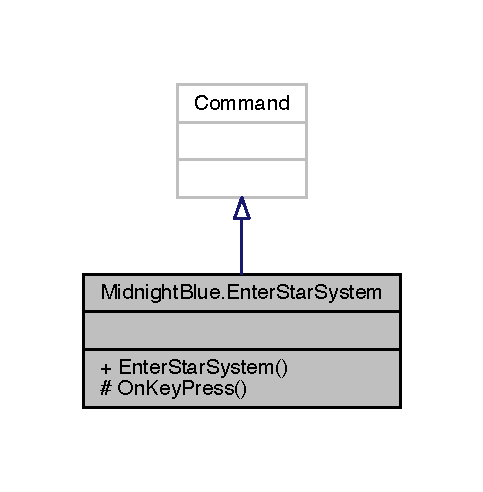
\includegraphics[width=232pt]{class_midnight_blue_1_1_enter_star_system__inherit__graph}
\end{center}
\end{figure}


Collaboration diagram for Midnight\+Blue.\+Enter\+Star\+System\+:
\nopagebreak
\begin{figure}[H]
\begin{center}
\leavevmode
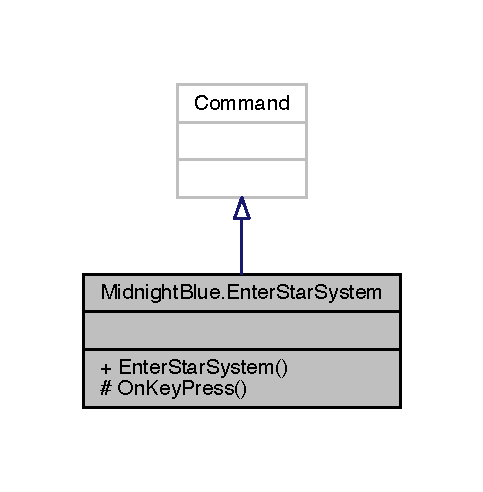
\includegraphics[width=232pt]{class_midnight_blue_1_1_enter_star_system__coll__graph}
\end{center}
\end{figure}
\subsection*{Public Member Functions}
\begin{DoxyCompactItemize}
\item 
\hyperlink{class_midnight_blue_1_1_enter_star_system_a6bea0a7daba691c1b46238114b347377}{Enter\+Star\+System} (Keys key, Command\+Type type)
\begin{DoxyCompactList}\small\item\em Initializes a new instance of the T\+:\+Midnight\+Blue.\+Enter\+Star\+System class. \end{DoxyCompactList}\end{DoxyCompactItemize}
\subsection*{Protected Member Functions}
\begin{DoxyCompactItemize}
\item 
override void \hyperlink{class_midnight_blue_1_1_enter_star_system_a1cf84a93760ef0cda918915ec8acfa4d}{On\+Key\+Press} (Entity e)
\begin{DoxyCompactList}\small\item\em Enters the collided with star system on keypress \end{DoxyCompactList}\end{DoxyCompactItemize}


\subsection{Detailed Description}
Enters a star system scene from the galaxy view 



\subsection{Constructor \& Destructor Documentation}
\hypertarget{class_midnight_blue_1_1_enter_star_system_a6bea0a7daba691c1b46238114b347377}{}\label{class_midnight_blue_1_1_enter_star_system_a6bea0a7daba691c1b46238114b347377} 
\index{Midnight\+Blue\+::\+Enter\+Star\+System@{Midnight\+Blue\+::\+Enter\+Star\+System}!Enter\+Star\+System@{Enter\+Star\+System}}
\index{Enter\+Star\+System@{Enter\+Star\+System}!Midnight\+Blue\+::\+Enter\+Star\+System@{Midnight\+Blue\+::\+Enter\+Star\+System}}
\subsubsection{\texorpdfstring{Enter\+Star\+System()}{EnterStarSystem()}}
{\footnotesize\ttfamily Midnight\+Blue.\+Enter\+Star\+System.\+Enter\+Star\+System (\begin{DoxyParamCaption}\item[{Keys}]{key,  }\item[{Command\+Type}]{type }\end{DoxyParamCaption})\hspace{0.3cm}{\ttfamily [inline]}}



Initializes a new instance of the T\+:\+Midnight\+Blue.\+Enter\+Star\+System class. 


\begin{DoxyParams}{Parameters}
{\em key} & Key to assign to.\\
\hline
{\em type} & Trigger type.\\
\hline
\end{DoxyParams}


\subsection{Member Function Documentation}
\hypertarget{class_midnight_blue_1_1_enter_star_system_a1cf84a93760ef0cda918915ec8acfa4d}{}\label{class_midnight_blue_1_1_enter_star_system_a1cf84a93760ef0cda918915ec8acfa4d} 
\index{Midnight\+Blue\+::\+Enter\+Star\+System@{Midnight\+Blue\+::\+Enter\+Star\+System}!On\+Key\+Press@{On\+Key\+Press}}
\index{On\+Key\+Press@{On\+Key\+Press}!Midnight\+Blue\+::\+Enter\+Star\+System@{Midnight\+Blue\+::\+Enter\+Star\+System}}
\subsubsection{\texorpdfstring{On\+Key\+Press()}{OnKeyPress()}}
{\footnotesize\ttfamily override void Midnight\+Blue.\+Enter\+Star\+System.\+On\+Key\+Press (\begin{DoxyParamCaption}\item[{Entity}]{e }\end{DoxyParamCaption})\hspace{0.3cm}{\ttfamily [inline]}, {\ttfamily [protected]}}



Enters the collided with star system on keypress 


\begin{DoxyParams}{Parameters}
{\em e} & E.\\
\hline
\end{DoxyParams}


The documentation for this class was generated from the following file\+:\begin{DoxyCompactItemize}
\item 
Shared/src/\+Game/\+Commands/Ship\+Commands.\+cs\end{DoxyCompactItemize}

\hypertarget{class_midnight_blue_1_1_fuel}{}\section{Midnight\+Blue.\+Fuel Class Reference}
\label{class_midnight_blue_1_1_fuel}\index{Midnight\+Blue.\+Fuel@{Midnight\+Blue.\+Fuel}}


\hyperlink{class_midnight_blue_1_1_fuel}{Fuel} used in the ships normal thruster drive  




Inheritance diagram for Midnight\+Blue.\+Fuel\+:
\nopagebreak
\begin{figure}[H]
\begin{center}
\leavevmode
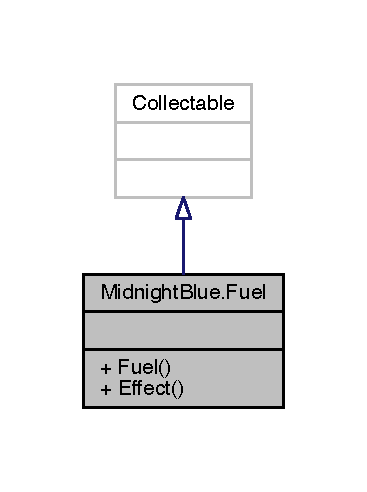
\includegraphics[width=176pt]{class_midnight_blue_1_1_fuel__inherit__graph}
\end{center}
\end{figure}


Collaboration diagram for Midnight\+Blue.\+Fuel\+:
\nopagebreak
\begin{figure}[H]
\begin{center}
\leavevmode
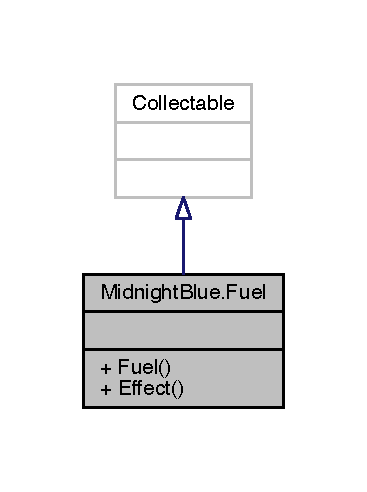
\includegraphics[width=176pt]{class_midnight_blue_1_1_fuel__coll__graph}
\end{center}
\end{figure}
\subsection*{Public Member Functions}
\begin{DoxyCompactItemize}
\item 
\hyperlink{class_midnight_blue_1_1_fuel_a44747305c7b7d4572d23fd764e568fc1}{Fuel} (int initial\+Count)
\begin{DoxyCompactList}\small\item\em Initializes a new instance of the T\+:\+Midnight\+Blue.\+Fuel class. \end{DoxyCompactList}\item 
override void \hyperlink{class_midnight_blue_1_1_fuel_a9ab52c79211ec8cdcc9389f772615ac0}{Effect} (Entity entity)
\begin{DoxyCompactList}\small\item\em Has no effect on the entity \end{DoxyCompactList}\end{DoxyCompactItemize}


\subsection{Detailed Description}
\hyperlink{class_midnight_blue_1_1_fuel}{Fuel} used in the ships normal thruster drive 



\subsection{Constructor \& Destructor Documentation}
\hypertarget{class_midnight_blue_1_1_fuel_a44747305c7b7d4572d23fd764e568fc1}{}\label{class_midnight_blue_1_1_fuel_a44747305c7b7d4572d23fd764e568fc1} 
\index{Midnight\+Blue\+::\+Fuel@{Midnight\+Blue\+::\+Fuel}!Fuel@{Fuel}}
\index{Fuel@{Fuel}!Midnight\+Blue\+::\+Fuel@{Midnight\+Blue\+::\+Fuel}}
\subsubsection{\texorpdfstring{Fuel()}{Fuel()}}
{\footnotesize\ttfamily Midnight\+Blue.\+Fuel.\+Fuel (\begin{DoxyParamCaption}\item[{int}]{initial\+Count }\end{DoxyParamCaption})\hspace{0.3cm}{\ttfamily [inline]}}



Initializes a new instance of the T\+:\+Midnight\+Blue.\+Fuel class. 


\begin{DoxyParams}{Parameters}
{\em initial\+Count} & Initial amount of fuel.\\
\hline
\end{DoxyParams}


\subsection{Member Function Documentation}
\hypertarget{class_midnight_blue_1_1_fuel_a9ab52c79211ec8cdcc9389f772615ac0}{}\label{class_midnight_blue_1_1_fuel_a9ab52c79211ec8cdcc9389f772615ac0} 
\index{Midnight\+Blue\+::\+Fuel@{Midnight\+Blue\+::\+Fuel}!Effect@{Effect}}
\index{Effect@{Effect}!Midnight\+Blue\+::\+Fuel@{Midnight\+Blue\+::\+Fuel}}
\subsubsection{\texorpdfstring{Effect()}{Effect()}}
{\footnotesize\ttfamily override void Midnight\+Blue.\+Fuel.\+Effect (\begin{DoxyParamCaption}\item[{Entity}]{entity }\end{DoxyParamCaption})\hspace{0.3cm}{\ttfamily [inline]}}



Has no effect on the entity 


\begin{DoxyParams}{Parameters}
{\em entity} & Entity.\\
\hline
\end{DoxyParams}


The documentation for this class was generated from the following file\+:\begin{DoxyCompactItemize}
\item 
Shared/src/\+Game/\+Inventory/Fuel.\+cs\end{DoxyCompactItemize}

\hypertarget{class_midnight_blue_1_1_galaxy_builder}{}\section{Midnight\+Blue.\+Galaxy\+Builder Class Reference}
\label{class_midnight_blue_1_1_galaxy_builder}\index{Midnight\+Blue.\+Galaxy\+Builder@{Midnight\+Blue.\+Galaxy\+Builder}}


Collaboration diagram for Midnight\+Blue.\+Galaxy\+Builder\+:
\nopagebreak
\begin{figure}[H]
\begin{center}
\leavevmode
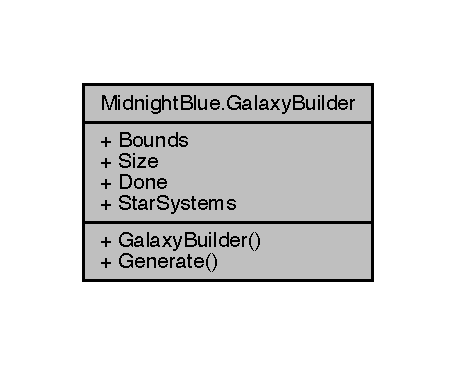
\includegraphics[width=219pt]{class_midnight_blue_1_1_galaxy_builder__coll__graph}
\end{center}
\end{figure}
\subsection*{Public Member Functions}
\begin{DoxyCompactItemize}
\item 
\hyperlink{class_midnight_blue_1_1_galaxy_builder_a926e49d9c54675035304d7506c02a0b9}{Galaxy\+Builder} (Content\+Manager content, int size, int seed=0)
\begin{DoxyCompactList}\small\item\em Initializes a new instance of the T\+:\+Midnight\+Blue.\+Galaxy\+Builder class. Does not actually generate the galaxy -\/ that\textquotesingle{}s done via \hyperlink{class_midnight_blue_1_1_galaxy_builder_aaa080e0108cf02709137b7eebb56ad1a}{Generate()} \end{DoxyCompactList}\item 
List$<$ \hyperlink{class_midnight_blue_1_1_star_system}{Star\+System} $>$ \hyperlink{class_midnight_blue_1_1_galaxy_builder_aaa080e0108cf02709137b7eebb56ad1a}{Generate} (int max\+Distance)
\begin{DoxyCompactList}\small\item\em Generates the galaxy with a specified max distance between stars. Takes a while so should be called only once per gameplay session. \end{DoxyCompactList}\end{DoxyCompactItemize}
\subsection*{Properties}
\begin{DoxyCompactItemize}
\item 
Rectangle \hyperlink{class_midnight_blue_1_1_galaxy_builder_a9051fa0f379b34dae5a6dcd287da7d9d}{Bounds}\hspace{0.3cm}{\ttfamily  \mbox{[}get\mbox{]}}
\begin{DoxyCompactList}\small\item\em Gets the bounding rectangle of the galaxy. \end{DoxyCompactList}\item 
int \hyperlink{class_midnight_blue_1_1_galaxy_builder_a295af2d47a68bdac0845f3540c815a63}{Size}\hspace{0.3cm}{\ttfamily  \mbox{[}get\mbox{]}}
\begin{DoxyCompactList}\small\item\em Gets the number of star systems the galaxy has. \end{DoxyCompactList}\item 
bool \hyperlink{class_midnight_blue_1_1_galaxy_builder_a4b496c6930a56d2469c21acb54ff23ec}{Done}\hspace{0.3cm}{\ttfamily  \mbox{[}get\mbox{]}}
\begin{DoxyCompactList}\small\item\em Gets a value indicating whether this T\+:\+Midnight\+Blue.\+Galaxy\+Builder is done generating. \end{DoxyCompactList}\item 
List$<$ \hyperlink{class_midnight_blue_1_1_star_system}{Star\+System} $>$ \hyperlink{class_midnight_blue_1_1_galaxy_builder_a85ce4bbc7de1c14ad7e7f0af3e92c1a1}{Star\+Systems}\hspace{0.3cm}{\ttfamily  \mbox{[}get\mbox{]}}
\begin{DoxyCompactList}\small\item\em Gets the star system list. \end{DoxyCompactList}\end{DoxyCompactItemize}


\subsection{Constructor \& Destructor Documentation}
\hypertarget{class_midnight_blue_1_1_galaxy_builder_a926e49d9c54675035304d7506c02a0b9}{}\label{class_midnight_blue_1_1_galaxy_builder_a926e49d9c54675035304d7506c02a0b9} 
\index{Midnight\+Blue\+::\+Galaxy\+Builder@{Midnight\+Blue\+::\+Galaxy\+Builder}!Galaxy\+Builder@{Galaxy\+Builder}}
\index{Galaxy\+Builder@{Galaxy\+Builder}!Midnight\+Blue\+::\+Galaxy\+Builder@{Midnight\+Blue\+::\+Galaxy\+Builder}}
\subsubsection{\texorpdfstring{Galaxy\+Builder()}{GalaxyBuilder()}}
{\footnotesize\ttfamily Midnight\+Blue.\+Galaxy\+Builder.\+Galaxy\+Builder (\begin{DoxyParamCaption}\item[{Content\+Manager}]{content,  }\item[{int}]{size,  }\item[{int}]{seed = {\ttfamily 0} }\end{DoxyParamCaption})\hspace{0.3cm}{\ttfamily [inline]}}



Initializes a new instance of the T\+:\+Midnight\+Blue.\+Galaxy\+Builder class. Does not actually generate the galaxy -\/ that\textquotesingle{}s done via \hyperlink{class_midnight_blue_1_1_galaxy_builder_aaa080e0108cf02709137b7eebb56ad1a}{Generate()} 


\begin{DoxyParams}{Parameters}
{\em content} & Content manager to use for loading resources.\\
\hline
{\em size} & Number of star systems to generate.\\
\hline
{\em seed} & Seed to use for generation.\\
\hline
\end{DoxyParams}


\subsection{Member Function Documentation}
\hypertarget{class_midnight_blue_1_1_galaxy_builder_aaa080e0108cf02709137b7eebb56ad1a}{}\label{class_midnight_blue_1_1_galaxy_builder_aaa080e0108cf02709137b7eebb56ad1a} 
\index{Midnight\+Blue\+::\+Galaxy\+Builder@{Midnight\+Blue\+::\+Galaxy\+Builder}!Generate@{Generate}}
\index{Generate@{Generate}!Midnight\+Blue\+::\+Galaxy\+Builder@{Midnight\+Blue\+::\+Galaxy\+Builder}}
\subsubsection{\texorpdfstring{Generate()}{Generate()}}
{\footnotesize\ttfamily List$<$\hyperlink{class_midnight_blue_1_1_star_system}{Star\+System}$>$ Midnight\+Blue.\+Galaxy\+Builder.\+Generate (\begin{DoxyParamCaption}\item[{int}]{max\+Distance }\end{DoxyParamCaption})\hspace{0.3cm}{\ttfamily [inline]}}



Generates the galaxy with a specified max distance between stars. Takes a while so should be called only once per gameplay session. 


\begin{DoxyParams}{Parameters}
{\em max\+Distance} & Max distance between generated star systems.\\
\hline
\end{DoxyParams}
Here is the caller graph for this function\+:
\nopagebreak
\begin{figure}[H]
\begin{center}
\leavevmode
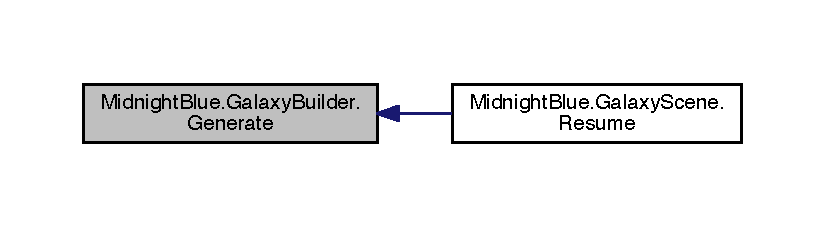
\includegraphics[width=350pt]{class_midnight_blue_1_1_galaxy_builder_aaa080e0108cf02709137b7eebb56ad1a_icgraph}
\end{center}
\end{figure}


\subsection{Property Documentation}
\hypertarget{class_midnight_blue_1_1_galaxy_builder_a9051fa0f379b34dae5a6dcd287da7d9d}{}\label{class_midnight_blue_1_1_galaxy_builder_a9051fa0f379b34dae5a6dcd287da7d9d} 
\index{Midnight\+Blue\+::\+Galaxy\+Builder@{Midnight\+Blue\+::\+Galaxy\+Builder}!Bounds@{Bounds}}
\index{Bounds@{Bounds}!Midnight\+Blue\+::\+Galaxy\+Builder@{Midnight\+Blue\+::\+Galaxy\+Builder}}
\subsubsection{\texorpdfstring{Bounds}{Bounds}}
{\footnotesize\ttfamily Rectangle Midnight\+Blue.\+Galaxy\+Builder.\+Bounds\hspace{0.3cm}{\ttfamily [get]}}



Gets the bounding rectangle of the galaxy. 

The bounds.\hypertarget{class_midnight_blue_1_1_galaxy_builder_a4b496c6930a56d2469c21acb54ff23ec}{}\label{class_midnight_blue_1_1_galaxy_builder_a4b496c6930a56d2469c21acb54ff23ec} 
\index{Midnight\+Blue\+::\+Galaxy\+Builder@{Midnight\+Blue\+::\+Galaxy\+Builder}!Done@{Done}}
\index{Done@{Done}!Midnight\+Blue\+::\+Galaxy\+Builder@{Midnight\+Blue\+::\+Galaxy\+Builder}}
\subsubsection{\texorpdfstring{Done}{Done}}
{\footnotesize\ttfamily bool Midnight\+Blue.\+Galaxy\+Builder.\+Done\hspace{0.3cm}{\ttfamily [get]}}



Gets a value indicating whether this T\+:\+Midnight\+Blue.\+Galaxy\+Builder is done generating. 

{\ttfamily true} if done; otherwise, {\ttfamily false}.\hypertarget{class_midnight_blue_1_1_galaxy_builder_a295af2d47a68bdac0845f3540c815a63}{}\label{class_midnight_blue_1_1_galaxy_builder_a295af2d47a68bdac0845f3540c815a63} 
\index{Midnight\+Blue\+::\+Galaxy\+Builder@{Midnight\+Blue\+::\+Galaxy\+Builder}!Size@{Size}}
\index{Size@{Size}!Midnight\+Blue\+::\+Galaxy\+Builder@{Midnight\+Blue\+::\+Galaxy\+Builder}}
\subsubsection{\texorpdfstring{Size}{Size}}
{\footnotesize\ttfamily int Midnight\+Blue.\+Galaxy\+Builder.\+Size\hspace{0.3cm}{\ttfamily [get]}}



Gets the number of star systems the galaxy has. 

The number of star systems.\hypertarget{class_midnight_blue_1_1_galaxy_builder_a85ce4bbc7de1c14ad7e7f0af3e92c1a1}{}\label{class_midnight_blue_1_1_galaxy_builder_a85ce4bbc7de1c14ad7e7f0af3e92c1a1} 
\index{Midnight\+Blue\+::\+Galaxy\+Builder@{Midnight\+Blue\+::\+Galaxy\+Builder}!Star\+Systems@{Star\+Systems}}
\index{Star\+Systems@{Star\+Systems}!Midnight\+Blue\+::\+Galaxy\+Builder@{Midnight\+Blue\+::\+Galaxy\+Builder}}
\subsubsection{\texorpdfstring{Star\+Systems}{StarSystems}}
{\footnotesize\ttfamily List$<$\hyperlink{class_midnight_blue_1_1_star_system}{Star\+System}$>$ Midnight\+Blue.\+Galaxy\+Builder.\+Star\+Systems\hspace{0.3cm}{\ttfamily [get]}}



Gets the star system list. 

The star systems.

The documentation for this class was generated from the following file\+:\begin{DoxyCompactItemize}
\item 
Shared/src/\+Game/\+Environment/Galaxy\+Builder.\+cs\end{DoxyCompactItemize}

\hypertarget{class_midnight_blue_1_1_galaxy_hud}{}\section{Midnight\+Blue.\+Galaxy\+Hud Class Reference}
\label{class_midnight_blue_1_1_galaxy_hud}\index{Midnight\+Blue.\+Galaxy\+Hud@{Midnight\+Blue.\+Galaxy\+Hud}}


H\+UD to show in the galaxy view.  




Inheritance diagram for Midnight\+Blue.\+Galaxy\+Hud\+:
\nopagebreak
\begin{figure}[H]
\begin{center}
\leavevmode
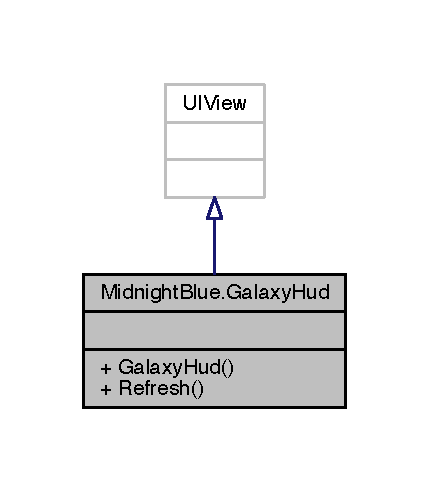
\includegraphics[width=206pt]{class_midnight_blue_1_1_galaxy_hud__inherit__graph}
\end{center}
\end{figure}


Collaboration diagram for Midnight\+Blue.\+Galaxy\+Hud\+:
\nopagebreak
\begin{figure}[H]
\begin{center}
\leavevmode
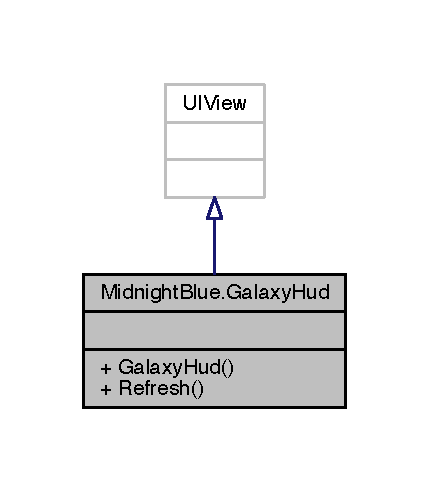
\includegraphics[width=206pt]{class_midnight_blue_1_1_galaxy_hud__coll__graph}
\end{center}
\end{figure}
\subsection*{Public Member Functions}
\begin{DoxyCompactItemize}
\item 
\hyperlink{class_midnight_blue_1_1_galaxy_hud_a6f15257e5bc5bbc67cac3888f075ea29}{Galaxy\+Hud} (Content\+Manager content)
\begin{DoxyCompactList}\small\item\em Initializes a new instance of the T\+:\+M\+B2\+D.\+Galaxy\+Hud class. \end{DoxyCompactList}\item 
void \hyperlink{class_midnight_blue_1_1_galaxy_hud_aea2d04b212188a2e729ea327b7da0449}{Refresh} (\hyperlink{class_m_b2_d_1_1_entity_component_1_1_inventory}{Inventory} inventory)
\begin{DoxyCompactList}\small\item\em Refreshed the H\+UD with the specified inventory values. \end{DoxyCompactList}\end{DoxyCompactItemize}
\subsection*{Additional Inherited Members}


\subsection{Detailed Description}
H\+UD to show in the galaxy view. 



\subsection{Constructor \& Destructor Documentation}
\hypertarget{class_midnight_blue_1_1_galaxy_hud_a6f15257e5bc5bbc67cac3888f075ea29}{}\label{class_midnight_blue_1_1_galaxy_hud_a6f15257e5bc5bbc67cac3888f075ea29} 
\index{Midnight\+Blue\+::\+Galaxy\+Hud@{Midnight\+Blue\+::\+Galaxy\+Hud}!Galaxy\+Hud@{Galaxy\+Hud}}
\index{Galaxy\+Hud@{Galaxy\+Hud}!Midnight\+Blue\+::\+Galaxy\+Hud@{Midnight\+Blue\+::\+Galaxy\+Hud}}
\subsubsection{\texorpdfstring{Galaxy\+Hud()}{GalaxyHud()}}
{\footnotesize\ttfamily Midnight\+Blue.\+Galaxy\+Hud.\+Galaxy\+Hud (\begin{DoxyParamCaption}\item[{Content\+Manager}]{content }\end{DoxyParamCaption})\hspace{0.3cm}{\ttfamily [inline]}}



Initializes a new instance of the T\+:\+M\+B2\+D.\+Galaxy\+Hud class. 


\begin{DoxyParams}{Parameters}
{\em content} & Content to use in loading fonts and textures.\\
\hline
\end{DoxyParams}
Here is the call graph for this function\+:
\nopagebreak
\begin{figure}[H]
\begin{center}
\leavevmode
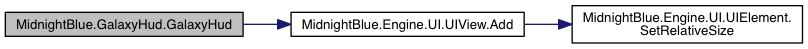
\includegraphics[width=350pt]{class_midnight_blue_1_1_galaxy_hud_a6f15257e5bc5bbc67cac3888f075ea29_cgraph}
\end{center}
\end{figure}


\subsection{Member Function Documentation}
\hypertarget{class_midnight_blue_1_1_galaxy_hud_aea2d04b212188a2e729ea327b7da0449}{}\label{class_midnight_blue_1_1_galaxy_hud_aea2d04b212188a2e729ea327b7da0449} 
\index{Midnight\+Blue\+::\+Galaxy\+Hud@{Midnight\+Blue\+::\+Galaxy\+Hud}!Refresh@{Refresh}}
\index{Refresh@{Refresh}!Midnight\+Blue\+::\+Galaxy\+Hud@{Midnight\+Blue\+::\+Galaxy\+Hud}}
\subsubsection{\texorpdfstring{Refresh()}{Refresh()}}
{\footnotesize\ttfamily void Midnight\+Blue.\+Galaxy\+Hud.\+Refresh (\begin{DoxyParamCaption}\item[{\hyperlink{class_m_b2_d_1_1_entity_component_1_1_inventory}{Inventory}}]{inventory }\end{DoxyParamCaption})\hspace{0.3cm}{\ttfamily [inline]}}



Refreshed the H\+UD with the specified inventory values. 


\begin{DoxyParams}{Parameters}
{\em inventory} & Inventory to use to refresh the display.\\
\hline
\end{DoxyParams}
Here is the caller graph for this function\+:
\nopagebreak
\begin{figure}[H]
\begin{center}
\leavevmode
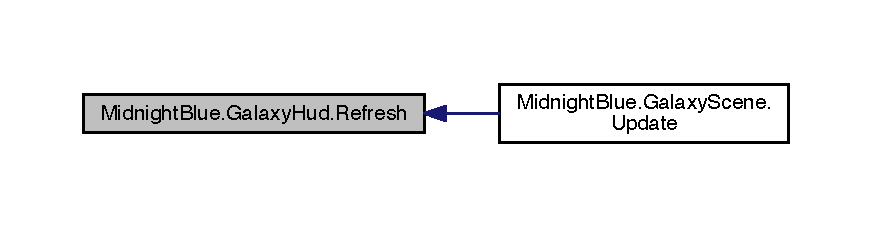
\includegraphics[width=350pt]{class_midnight_blue_1_1_galaxy_hud_aea2d04b212188a2e729ea327b7da0449_icgraph}
\end{center}
\end{figure}


The documentation for this class was generated from the following file\+:\begin{DoxyCompactItemize}
\item 
Shared/src/\+Game/\+U\+I\+Views/Galaxy\+Hud.\+cs\end{DoxyCompactItemize}

\hypertarget{class_midnight_blue_1_1_galaxy_render_system}{}\section{Midnight\+Blue.\+Galaxy\+Render\+System Class Reference}
\label{class_midnight_blue_1_1_galaxy_render_system}\index{Midnight\+Blue.\+Galaxy\+Render\+System@{Midnight\+Blue.\+Galaxy\+Render\+System}}


Renders all information into the main H\+UD\textquotesingle{}s list box on the hovered star system. Also displays the name of all the star systems planets.  




Inheritance diagram for Midnight\+Blue.\+Galaxy\+Render\+System\+:
\nopagebreak
\begin{figure}[H]
\begin{center}
\leavevmode
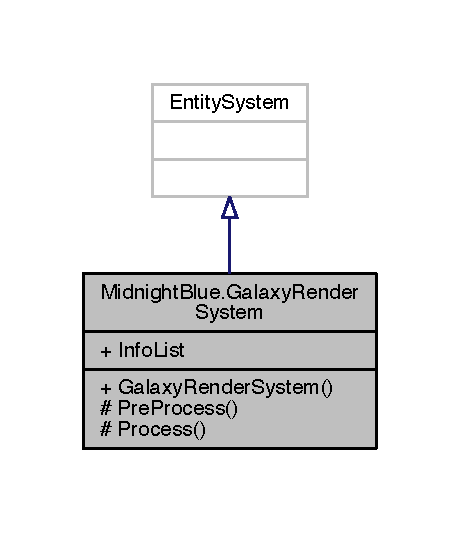
\includegraphics[width=221pt]{class_midnight_blue_1_1_galaxy_render_system__inherit__graph}
\end{center}
\end{figure}


Collaboration diagram for Midnight\+Blue.\+Galaxy\+Render\+System\+:
\nopagebreak
\begin{figure}[H]
\begin{center}
\leavevmode
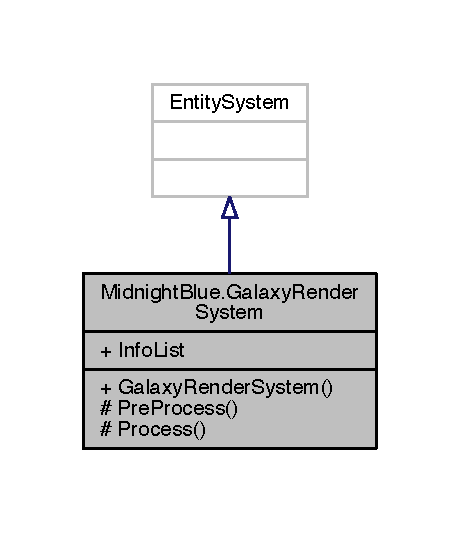
\includegraphics[width=221pt]{class_midnight_blue_1_1_galaxy_render_system__coll__graph}
\end{center}
\end{figure}
\subsection*{Public Member Functions}
\begin{DoxyCompactItemize}
\item 
\hyperlink{class_midnight_blue_1_1_galaxy_render_system_aee5d42f0287d1bfed669e2a2656c5c28}{Galaxy\+Render\+System} (Sprite\+Batch sprite\+Batch, Content\+Manager content)
\begin{DoxyCompactList}\small\item\em Initializes a new instance of the T\+:\+Midnight\+Blue.\+Galaxy\+Render\+System class. \end{DoxyCompactList}\end{DoxyCompactItemize}
\subsection*{Protected Member Functions}
\begin{DoxyCompactItemize}
\item 
override void \hyperlink{class_midnight_blue_1_1_galaxy_render_system_a269f042fe0c55e47f3b23cc1930ed71a}{Pre\+Process} ()
\begin{DoxyCompactList}\small\item\em Clears the starsystems info list before processing all entities. \end{DoxyCompactList}\item 
override void \hyperlink{class_midnight_blue_1_1_galaxy_render_system_aabbf61a4bcfb7c026d2d0c9fbe90569f}{Process} (Entity entity)
\begin{DoxyCompactList}\small\item\em Checks for collisions with a star system in the galaxy view and renders any information associated with that star re\+:planets. \end{DoxyCompactList}\end{DoxyCompactItemize}
\subsection*{Properties}
\begin{DoxyCompactItemize}
\item 
List$<$ string $>$ \hyperlink{class_midnight_blue_1_1_galaxy_render_system_a2f252c64ec38b5bcf20c6b276fd5809b}{Info\+List}\hspace{0.3cm}{\ttfamily  \mbox{[}get\mbox{]}}
\begin{DoxyCompactList}\small\item\em Gets the list of all planets in the star system\textquotesingle{}s information. \end{DoxyCompactList}\end{DoxyCompactItemize}


\subsection{Detailed Description}
Renders all information into the main H\+UD\textquotesingle{}s list box on the hovered star system. Also displays the name of all the star systems planets. 



\subsection{Constructor \& Destructor Documentation}
\hypertarget{class_midnight_blue_1_1_galaxy_render_system_aee5d42f0287d1bfed669e2a2656c5c28}{}\label{class_midnight_blue_1_1_galaxy_render_system_aee5d42f0287d1bfed669e2a2656c5c28} 
\index{Midnight\+Blue\+::\+Galaxy\+Render\+System@{Midnight\+Blue\+::\+Galaxy\+Render\+System}!Galaxy\+Render\+System@{Galaxy\+Render\+System}}
\index{Galaxy\+Render\+System@{Galaxy\+Render\+System}!Midnight\+Blue\+::\+Galaxy\+Render\+System@{Midnight\+Blue\+::\+Galaxy\+Render\+System}}
\subsubsection{\texorpdfstring{Galaxy\+Render\+System()}{GalaxyRenderSystem()}}
{\footnotesize\ttfamily Midnight\+Blue.\+Galaxy\+Render\+System.\+Galaxy\+Render\+System (\begin{DoxyParamCaption}\item[{Sprite\+Batch}]{sprite\+Batch,  }\item[{Content\+Manager}]{content }\end{DoxyParamCaption})\hspace{0.3cm}{\ttfamily [inline]}}



Initializes a new instance of the T\+:\+Midnight\+Blue.\+Galaxy\+Render\+System class. 


\begin{DoxyParams}{Parameters}
{\em sprite\+Batch} & Sprite batch to draw to.\\
\hline
{\em content} & Content to load fonts from.\\
\hline
\end{DoxyParams}


\subsection{Member Function Documentation}
\hypertarget{class_midnight_blue_1_1_galaxy_render_system_a269f042fe0c55e47f3b23cc1930ed71a}{}\label{class_midnight_blue_1_1_galaxy_render_system_a269f042fe0c55e47f3b23cc1930ed71a} 
\index{Midnight\+Blue\+::\+Galaxy\+Render\+System@{Midnight\+Blue\+::\+Galaxy\+Render\+System}!Pre\+Process@{Pre\+Process}}
\index{Pre\+Process@{Pre\+Process}!Midnight\+Blue\+::\+Galaxy\+Render\+System@{Midnight\+Blue\+::\+Galaxy\+Render\+System}}
\subsubsection{\texorpdfstring{Pre\+Process()}{PreProcess()}}
{\footnotesize\ttfamily override void Midnight\+Blue.\+Galaxy\+Render\+System.\+Pre\+Process (\begin{DoxyParamCaption}{ }\end{DoxyParamCaption})\hspace{0.3cm}{\ttfamily [inline]}, {\ttfamily [protected]}}



Clears the starsystems info list before processing all entities. 

\hypertarget{class_midnight_blue_1_1_galaxy_render_system_aabbf61a4bcfb7c026d2d0c9fbe90569f}{}\label{class_midnight_blue_1_1_galaxy_render_system_aabbf61a4bcfb7c026d2d0c9fbe90569f} 
\index{Midnight\+Blue\+::\+Galaxy\+Render\+System@{Midnight\+Blue\+::\+Galaxy\+Render\+System}!Process@{Process}}
\index{Process@{Process}!Midnight\+Blue\+::\+Galaxy\+Render\+System@{Midnight\+Blue\+::\+Galaxy\+Render\+System}}
\subsubsection{\texorpdfstring{Process()}{Process()}}
{\footnotesize\ttfamily override void Midnight\+Blue.\+Galaxy\+Render\+System.\+Process (\begin{DoxyParamCaption}\item[{Entity}]{entity }\end{DoxyParamCaption})\hspace{0.3cm}{\ttfamily [inline]}, {\ttfamily [protected]}}



Checks for collisions with a star system in the galaxy view and renders any information associated with that star re\+:planets. 


\begin{DoxyParams}{Parameters}
{\em entity} & Entity to check collisions with.\\
\hline
\end{DoxyParams}


\subsection{Property Documentation}
\hypertarget{class_midnight_blue_1_1_galaxy_render_system_a2f252c64ec38b5bcf20c6b276fd5809b}{}\label{class_midnight_blue_1_1_galaxy_render_system_a2f252c64ec38b5bcf20c6b276fd5809b} 
\index{Midnight\+Blue\+::\+Galaxy\+Render\+System@{Midnight\+Blue\+::\+Galaxy\+Render\+System}!Info\+List@{Info\+List}}
\index{Info\+List@{Info\+List}!Midnight\+Blue\+::\+Galaxy\+Render\+System@{Midnight\+Blue\+::\+Galaxy\+Render\+System}}
\subsubsection{\texorpdfstring{Info\+List}{InfoList}}
{\footnotesize\ttfamily List$<$string$>$ Midnight\+Blue.\+Galaxy\+Render\+System.\+Info\+List\hspace{0.3cm}{\ttfamily [get]}}



Gets the list of all planets in the star system\textquotesingle{}s information. 

The info list.

The documentation for this class was generated from the following file\+:\begin{DoxyCompactItemize}
\item 
Shared/src/\+Game/\+Systems/Galaxy\+Render\+System.\+cs\end{DoxyCompactItemize}

\hypertarget{class_midnight_blue_1_1_galaxy_scene}{}\section{Midnight\+Blue.\+Galaxy\+Scene Class Reference}
\label{class_midnight_blue_1_1_galaxy_scene}\index{Midnight\+Blue.\+Galaxy\+Scene@{Midnight\+Blue.\+Galaxy\+Scene}}


The scene displayed at the galaxy view -\/ handles the control over all systems, loading, and content management for the scene.  




Inheritance diagram for Midnight\+Blue.\+Galaxy\+Scene\+:\nopagebreak
\begin{figure}[H]
\begin{center}
\leavevmode
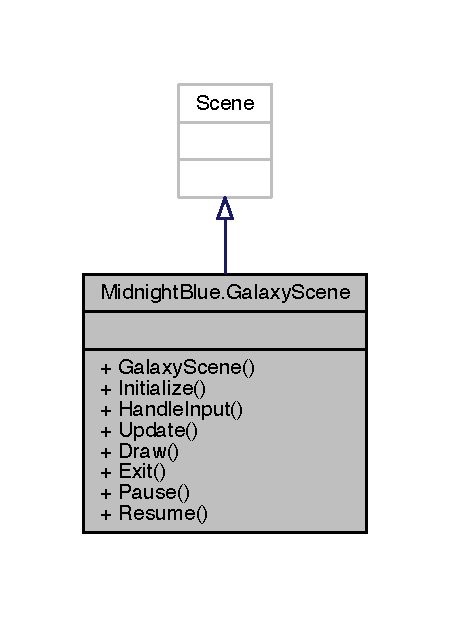
\includegraphics[width=217pt]{class_midnight_blue_1_1_galaxy_scene__inherit__graph}
\end{center}
\end{figure}


Collaboration diagram for Midnight\+Blue.\+Galaxy\+Scene\+:\nopagebreak
\begin{figure}[H]
\begin{center}
\leavevmode
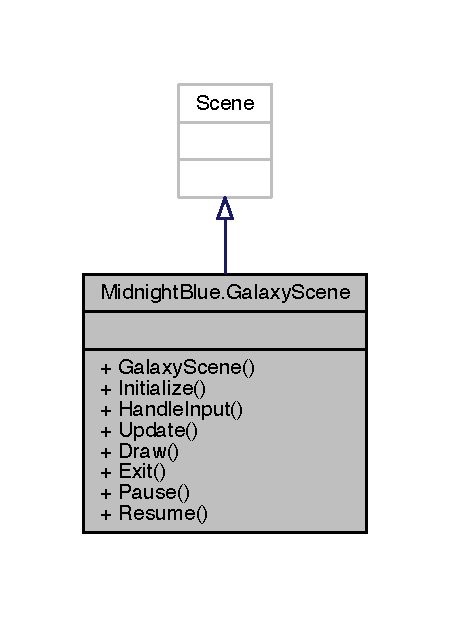
\includegraphics[width=217pt]{class_midnight_blue_1_1_galaxy_scene__coll__graph}
\end{center}
\end{figure}
\subsection*{Public Member Functions}
\begin{DoxyCompactItemize}
\item 
\hyperlink{class_midnight_blue_1_1_galaxy_scene_acdd82e3464ea18ca77bcf4694e9803a5}{Galaxy\+Scene} (\hyperlink{class_m_b2_d_1_1_entity_component_1_1_entity_map}{Entity\+Map} map, Content\+Manager content)
\begin{DoxyCompactList}\small\item\em Initializes a new instance of the T\+:\+M\+B2\+D.\+Galaxy\+Scene class. Loads all resources and sets up the galaxy for generation. \end{DoxyCompactList}\item 
override void \hyperlink{class_midnight_blue_1_1_galaxy_scene_a97d97e56a73d9a4b7caf6dd6ce86647e}{Initialize} ()
\begin{DoxyCompactList}\small\item\em Initializes the galaxy generation and background music -\/ sets up the players ship and the collision bounds. \end{DoxyCompactList}\item 
override void \hyperlink{class_midnight_blue_1_1_galaxy_scene_afd7f8c9f6d0cf6ded10299d4b0015c29}{Handle\+Input} ()
\begin{DoxyCompactList}\small\item\em Handles all input for the player ship and moves between galaxy and star system scenes if the player enters a star system. \end{DoxyCompactList}\item 
override void \hyperlink{class_midnight_blue_1_1_galaxy_scene_a9dfa66406143ed20f4d534c768f05a78}{Update} ()
\begin{DoxyCompactList}\small\item\em Updates the galaxy view and fuel consumption if not loading. \end{DoxyCompactList}\item 
override void \hyperlink{class_midnight_blue_1_1_galaxy_scene_a3646fcf97e067bac267d42aad66e71c4}{Draw} (Sprite\+Batch sprite\+Batch, Sprite\+Batch ui\+Sprite\+Batch)
\begin{DoxyCompactList}\small\item\em Draw the game world and UI to the specified sprite\+Batch and ui\+Sprite\+Batch. \end{DoxyCompactList}\item 
override void \hyperlink{class_midnight_blue_1_1_galaxy_scene_a7a96978e050da997330bcc0f3cd00f9e}{Exit} ()
\begin{DoxyCompactList}\small\item\em Exit this scene instantly. \end{DoxyCompactList}\item 
override void \hyperlink{class_midnight_blue_1_1_galaxy_scene_aeb44afaeda2cccd225e64908bb76bee4}{Pause} ()
\begin{DoxyCompactList}\small\item\em Fades the sound out when transitioning to another scene unless the next scene is the star system scene. \end{DoxyCompactList}\item 
override void \hyperlink{class_midnight_blue_1_1_galaxy_scene_ab641e6727cdb64dc6487e9a229521692}{Resume} ()
\begin{DoxyCompactList}\small\item\em Resets the physics environment when returning to the scene and rebuilds the galaxy from its cache. \end{DoxyCompactList}\end{DoxyCompactItemize}
\subsection*{Additional Inherited Members}


\subsection{Detailed Description}
The scene displayed at the galaxy view -\/ handles the control over all systems, loading, and content management for the scene. 



\subsection{Constructor \& Destructor Documentation}
\hypertarget{class_midnight_blue_1_1_galaxy_scene_acdd82e3464ea18ca77bcf4694e9803a5}{}\label{class_midnight_blue_1_1_galaxy_scene_acdd82e3464ea18ca77bcf4694e9803a5} 
\index{Midnight\+Blue\+::\+Galaxy\+Scene@{Midnight\+Blue\+::\+Galaxy\+Scene}!Galaxy\+Scene@{Galaxy\+Scene}}
\index{Galaxy\+Scene@{Galaxy\+Scene}!Midnight\+Blue\+::\+Galaxy\+Scene@{Midnight\+Blue\+::\+Galaxy\+Scene}}
\subsubsection{\texorpdfstring{Galaxy\+Scene()}{GalaxyScene()}}
{\footnotesize\ttfamily Midnight\+Blue.\+Galaxy\+Scene.\+Galaxy\+Scene (\begin{DoxyParamCaption}\item[{\hyperlink{class_m_b2_d_1_1_entity_component_1_1_entity_map}{Entity\+Map}}]{map,  }\item[{Content\+Manager}]{content }\end{DoxyParamCaption})\hspace{0.3cm}{\ttfamily [inline]}}



Initializes a new instance of the T\+:\+M\+B2\+D.\+Galaxy\+Scene class. Loads all resources and sets up the galaxy for generation. 


\begin{DoxyParams}{Parameters}
{\em map} & Game objects to use.\\
\hline
{\em content} & Content manager to use.\\
\hline
\end{DoxyParams}


\subsection{Member Function Documentation}
\hypertarget{class_midnight_blue_1_1_galaxy_scene_a3646fcf97e067bac267d42aad66e71c4}{}\label{class_midnight_blue_1_1_galaxy_scene_a3646fcf97e067bac267d42aad66e71c4} 
\index{Midnight\+Blue\+::\+Galaxy\+Scene@{Midnight\+Blue\+::\+Galaxy\+Scene}!Draw@{Draw}}
\index{Draw@{Draw}!Midnight\+Blue\+::\+Galaxy\+Scene@{Midnight\+Blue\+::\+Galaxy\+Scene}}
\subsubsection{\texorpdfstring{Draw()}{Draw()}}
{\footnotesize\ttfamily override void Midnight\+Blue.\+Galaxy\+Scene.\+Draw (\begin{DoxyParamCaption}\item[{Sprite\+Batch}]{sprite\+Batch,  }\item[{Sprite\+Batch}]{ui\+Sprite\+Batch }\end{DoxyParamCaption})\hspace{0.3cm}{\ttfamily [inline]}, {\ttfamily [virtual]}}



Draw the game world and UI to the specified sprite\+Batch and ui\+Sprite\+Batch. 


\begin{DoxyParams}{Parameters}
{\em sprite\+Batch} & Sprite batch for world-\/based entities.\\
\hline
{\em ui\+Sprite\+Batch} & User interface sprite batch.\\
\hline
\end{DoxyParams}


Implements \hyperlink{class_m_b2_d_1_1_scenes_1_1_scene_a932d33071ecb4c5187367825dba72324}{M\+B2\+D.\+Scenes.\+Scene}.

Here is the call graph for this function\+:\nopagebreak
\begin{figure}[H]
\begin{center}
\leavevmode
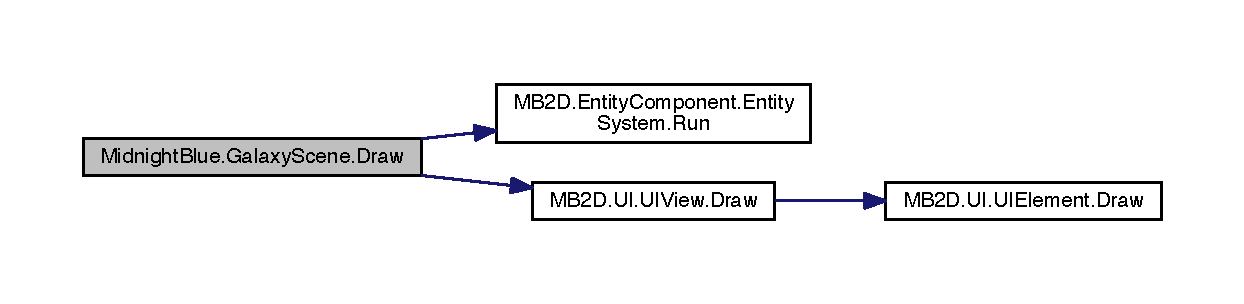
\includegraphics[width=350pt]{class_midnight_blue_1_1_galaxy_scene_a3646fcf97e067bac267d42aad66e71c4_cgraph}
\end{center}
\end{figure}
\hypertarget{class_midnight_blue_1_1_galaxy_scene_a7a96978e050da997330bcc0f3cd00f9e}{}\label{class_midnight_blue_1_1_galaxy_scene_a7a96978e050da997330bcc0f3cd00f9e} 
\index{Midnight\+Blue\+::\+Galaxy\+Scene@{Midnight\+Blue\+::\+Galaxy\+Scene}!Exit@{Exit}}
\index{Exit@{Exit}!Midnight\+Blue\+::\+Galaxy\+Scene@{Midnight\+Blue\+::\+Galaxy\+Scene}}
\subsubsection{\texorpdfstring{Exit()}{Exit()}}
{\footnotesize\ttfamily override void Midnight\+Blue.\+Galaxy\+Scene.\+Exit (\begin{DoxyParamCaption}{ }\end{DoxyParamCaption})\hspace{0.3cm}{\ttfamily [inline]}, {\ttfamily [virtual]}}



Exit this scene instantly. 



Implements \hyperlink{class_m_b2_d_1_1_scenes_1_1_scene_a099b79e16d23b67349847999d2336813}{M\+B2\+D.\+Scenes.\+Scene}.

\hypertarget{class_midnight_blue_1_1_galaxy_scene_afd7f8c9f6d0cf6ded10299d4b0015c29}{}\label{class_midnight_blue_1_1_galaxy_scene_afd7f8c9f6d0cf6ded10299d4b0015c29} 
\index{Midnight\+Blue\+::\+Galaxy\+Scene@{Midnight\+Blue\+::\+Galaxy\+Scene}!Handle\+Input@{Handle\+Input}}
\index{Handle\+Input@{Handle\+Input}!Midnight\+Blue\+::\+Galaxy\+Scene@{Midnight\+Blue\+::\+Galaxy\+Scene}}
\subsubsection{\texorpdfstring{Handle\+Input()}{HandleInput()}}
{\footnotesize\ttfamily override void Midnight\+Blue.\+Galaxy\+Scene.\+Handle\+Input (\begin{DoxyParamCaption}{ }\end{DoxyParamCaption})\hspace{0.3cm}{\ttfamily [inline]}, {\ttfamily [virtual]}}



Handles all input for the player ship and moves between galaxy and star system scenes if the player enters a star system. 



Implements \hyperlink{class_m_b2_d_1_1_scenes_1_1_scene_a476de5a885408d27ff151044d20738c8}{M\+B2\+D.\+Scenes.\+Scene}.

Here is the call graph for this function\+:\nopagebreak
\begin{figure}[H]
\begin{center}
\leavevmode
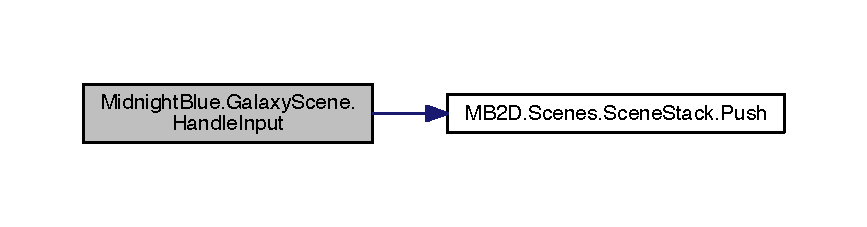
\includegraphics[width=350pt]{class_midnight_blue_1_1_galaxy_scene_afd7f8c9f6d0cf6ded10299d4b0015c29_cgraph}
\end{center}
\end{figure}
\hypertarget{class_midnight_blue_1_1_galaxy_scene_a97d97e56a73d9a4b7caf6dd6ce86647e}{}\label{class_midnight_blue_1_1_galaxy_scene_a97d97e56a73d9a4b7caf6dd6ce86647e} 
\index{Midnight\+Blue\+::\+Galaxy\+Scene@{Midnight\+Blue\+::\+Galaxy\+Scene}!Initialize@{Initialize}}
\index{Initialize@{Initialize}!Midnight\+Blue\+::\+Galaxy\+Scene@{Midnight\+Blue\+::\+Galaxy\+Scene}}
\subsubsection{\texorpdfstring{Initialize()}{Initialize()}}
{\footnotesize\ttfamily override void Midnight\+Blue.\+Galaxy\+Scene.\+Initialize (\begin{DoxyParamCaption}{ }\end{DoxyParamCaption})\hspace{0.3cm}{\ttfamily [inline]}, {\ttfamily [virtual]}}



Initializes the galaxy generation and background music -\/ sets up the players ship and the collision bounds. 



Implements \hyperlink{class_m_b2_d_1_1_scenes_1_1_scene_a081b4f8866936b495bdce388a7c96c25}{M\+B2\+D.\+Scenes.\+Scene}.

\hypertarget{class_midnight_blue_1_1_galaxy_scene_aeb44afaeda2cccd225e64908bb76bee4}{}\label{class_midnight_blue_1_1_galaxy_scene_aeb44afaeda2cccd225e64908bb76bee4} 
\index{Midnight\+Blue\+::\+Galaxy\+Scene@{Midnight\+Blue\+::\+Galaxy\+Scene}!Pause@{Pause}}
\index{Pause@{Pause}!Midnight\+Blue\+::\+Galaxy\+Scene@{Midnight\+Blue\+::\+Galaxy\+Scene}}
\subsubsection{\texorpdfstring{Pause()}{Pause()}}
{\footnotesize\ttfamily override void Midnight\+Blue.\+Galaxy\+Scene.\+Pause (\begin{DoxyParamCaption}{ }\end{DoxyParamCaption})\hspace{0.3cm}{\ttfamily [inline]}, {\ttfamily [virtual]}}



Fades the sound out when transitioning to another scene unless the next scene is the star system scene. 



Implements \hyperlink{class_m_b2_d_1_1_scenes_1_1_scene_a0661eff0223150fa8e9ea88145409e5d}{M\+B2\+D.\+Scenes.\+Scene}.

Here is the call graph for this function\+:\nopagebreak
\begin{figure}[H]
\begin{center}
\leavevmode
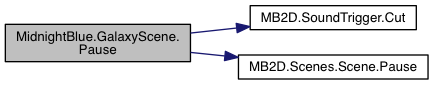
\includegraphics[width=350pt]{class_midnight_blue_1_1_galaxy_scene_aeb44afaeda2cccd225e64908bb76bee4_cgraph}
\end{center}
\end{figure}
\hypertarget{class_midnight_blue_1_1_galaxy_scene_ab641e6727cdb64dc6487e9a229521692}{}\label{class_midnight_blue_1_1_galaxy_scene_ab641e6727cdb64dc6487e9a229521692} 
\index{Midnight\+Blue\+::\+Galaxy\+Scene@{Midnight\+Blue\+::\+Galaxy\+Scene}!Resume@{Resume}}
\index{Resume@{Resume}!Midnight\+Blue\+::\+Galaxy\+Scene@{Midnight\+Blue\+::\+Galaxy\+Scene}}
\subsubsection{\texorpdfstring{Resume()}{Resume()}}
{\footnotesize\ttfamily override void Midnight\+Blue.\+Galaxy\+Scene.\+Resume (\begin{DoxyParamCaption}{ }\end{DoxyParamCaption})\hspace{0.3cm}{\ttfamily [inline]}, {\ttfamily [virtual]}}



Resets the physics environment when returning to the scene and rebuilds the galaxy from its cache. 



Implements \hyperlink{class_m_b2_d_1_1_scenes_1_1_scene_ad13639db22b059a1b714eefd9d927735}{M\+B2\+D.\+Scenes.\+Scene}.

Here is the call graph for this function\+:\nopagebreak
\begin{figure}[H]
\begin{center}
\leavevmode
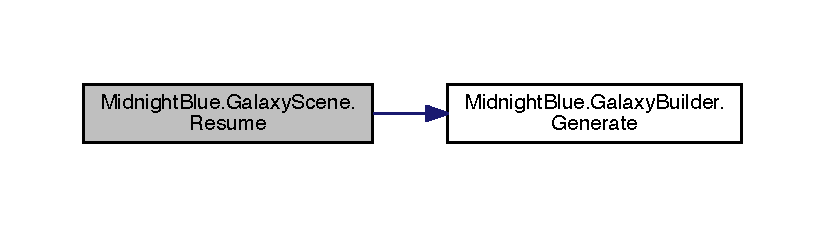
\includegraphics[width=350pt]{class_midnight_blue_1_1_galaxy_scene_ab641e6727cdb64dc6487e9a229521692_cgraph}
\end{center}
\end{figure}
\hypertarget{class_midnight_blue_1_1_galaxy_scene_a9dfa66406143ed20f4d534c768f05a78}{}\label{class_midnight_blue_1_1_galaxy_scene_a9dfa66406143ed20f4d534c768f05a78} 
\index{Midnight\+Blue\+::\+Galaxy\+Scene@{Midnight\+Blue\+::\+Galaxy\+Scene}!Update@{Update}}
\index{Update@{Update}!Midnight\+Blue\+::\+Galaxy\+Scene@{Midnight\+Blue\+::\+Galaxy\+Scene}}
\subsubsection{\texorpdfstring{Update()}{Update()}}
{\footnotesize\ttfamily override void Midnight\+Blue.\+Galaxy\+Scene.\+Update (\begin{DoxyParamCaption}{ }\end{DoxyParamCaption})\hspace{0.3cm}{\ttfamily [inline]}, {\ttfamily [virtual]}}



Updates the galaxy view and fuel consumption if not loading. 



Implements \hyperlink{class_m_b2_d_1_1_scenes_1_1_scene_a779de7c1ab23b698dcde3a228324a991}{M\+B2\+D.\+Scenes.\+Scene}.

Here is the call graph for this function\+:\nopagebreak
\begin{figure}[H]
\begin{center}
\leavevmode
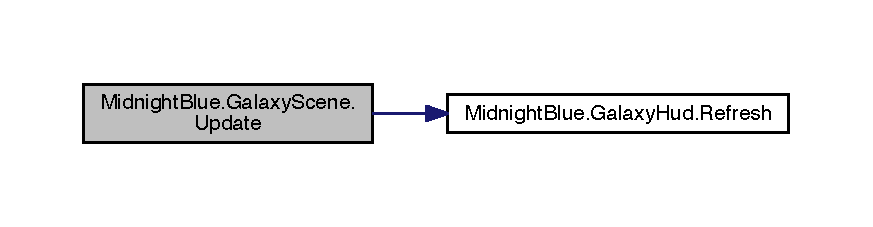
\includegraphics[width=350pt]{class_midnight_blue_1_1_galaxy_scene_a9dfa66406143ed20f4d534c768f05a78_cgraph}
\end{center}
\end{figure}


The documentation for this class was generated from the following file\+:\begin{DoxyCompactItemize}
\item 
Shared/src/\+Game/\+Scenes/Galaxy\+Scene.\+cs\end{DoxyCompactItemize}

\hypertarget{class_midnight_blue_1_1_testing_1_1_gen_test}{}\section{Midnight\+Blue.\+Testing.\+Gen\+Test Class Reference}
\label{class_midnight_blue_1_1_testing_1_1_gen_test}\index{Midnight\+Blue.\+Testing.\+Gen\+Test@{Midnight\+Blue.\+Testing.\+Gen\+Test}}


Collaboration diagram for Midnight\+Blue.\+Testing.\+Gen\+Test\+:\nopagebreak
\begin{figure}[H]
\begin{center}
\leavevmode
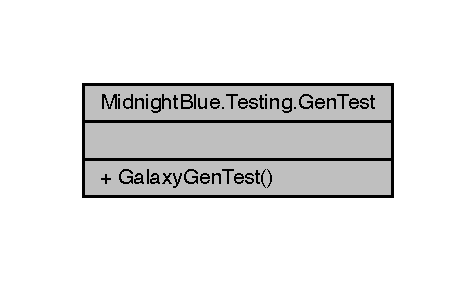
\includegraphics[width=228pt]{class_midnight_blue_1_1_testing_1_1_gen_test__coll__graph}
\end{center}
\end{figure}
\subsection*{Static Public Member Functions}
\begin{DoxyCompactItemize}
\item 
\hypertarget{class_midnight_blue_1_1_testing_1_1_gen_test_a9e196f4e8e4336758ed2c2099ace6d58}{}\label{class_midnight_blue_1_1_testing_1_1_gen_test_a9e196f4e8e4336758ed2c2099ace6d58} 
static void {\bfseries Galaxy\+Gen\+Test} (params string\mbox{[}$\,$\mbox{]} args)
\end{DoxyCompactItemize}


The documentation for this class was generated from the following file\+:\begin{DoxyCompactItemize}
\item 
Shared/src/\+Game/\+Tests/Gen\+Test.\+cs\end{DoxyCompactItemize}

\hypertarget{class_midnight_blue_1_1_init_scene}{}\section{Midnight\+Blue.\+Init\+Scene Class Reference}
\label{class_midnight_blue_1_1_init_scene}\index{Midnight\+Blue.\+Init\+Scene@{Midnight\+Blue.\+Init\+Scene}}


The scene shown at the title screen.  




Inheritance diagram for Midnight\+Blue.\+Init\+Scene\+:
\nopagebreak
\begin{figure}[H]
\begin{center}
\leavevmode
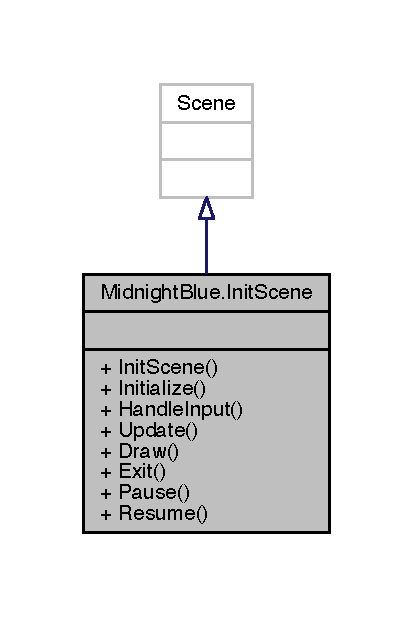
\includegraphics[width=217pt]{class_midnight_blue_1_1_init_scene__inherit__graph}
\end{center}
\end{figure}


Collaboration diagram for Midnight\+Blue.\+Init\+Scene\+:
\nopagebreak
\begin{figure}[H]
\begin{center}
\leavevmode
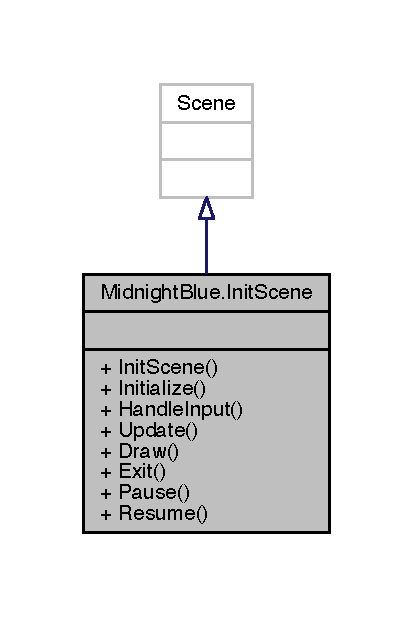
\includegraphics[width=217pt]{class_midnight_blue_1_1_init_scene__coll__graph}
\end{center}
\end{figure}
\subsection*{Public Member Functions}
\begin{DoxyCompactItemize}
\item 
\hyperlink{class_midnight_blue_1_1_init_scene_a6458d599d89e074484645974a1975f46}{Init\+Scene} (\hyperlink{class_m_b2_d_1_1_entity_component_1_1_entity_map}{Entity\+Map} map, Content\+Manager content)
\begin{DoxyCompactList}\small\item\em Initializes a new instance of the T\+:\+Midnight\+Blue.\+Init\+Scene class. Loads all blueprints and setup data. \end{DoxyCompactList}\item 
override void \hyperlink{class_midnight_blue_1_1_init_scene_a99eee8cc5dab8d7263591aeaa50144fb}{Initialize} ()
\begin{DoxyCompactList}\small\item\em Registers all blueprints to the Entity\+Map \end{DoxyCompactList}\item 
override void \hyperlink{class_midnight_blue_1_1_init_scene_a4a8d9c22193d334e41685ce62fa11dd9}{Handle\+Input} ()
\begin{DoxyCompactList}\small\item\em Handles the input for the scene. \end{DoxyCompactList}\item 
override void \hyperlink{class_midnight_blue_1_1_init_scene_ad87861fb4f2a30f5168f6133aa10d3f4}{Update} ()
\begin{DoxyCompactList}\small\item\em Updates the scene. \end{DoxyCompactList}\item 
override void \hyperlink{class_midnight_blue_1_1_init_scene_a5d6b21ff45a6c14edcf0bd8318133725}{Draw} (Sprite\+Batch sprite\+Batch, Sprite\+Batch ui\+Sprite\+Batch)
\begin{DoxyCompactList}\small\item\em Draws the scene to the ui\+Sprite\+Batch \end{DoxyCompactList}\item 
override void \hyperlink{class_midnight_blue_1_1_init_scene_a16fc773b06a711e1ba35dda44e3edc3e}{Exit} ()
\begin{DoxyCompactList}\small\item\em Exits the scene. \end{DoxyCompactList}\item 
override void \hyperlink{class_midnight_blue_1_1_init_scene_adbcab013e715e5c49ad09bcd0545d994}{Pause} ()
\begin{DoxyCompactList}\small\item\em Pauses the scene. \end{DoxyCompactList}\item 
override void \hyperlink{class_midnight_blue_1_1_init_scene_a01ade76252a492d20181bd2e00eb217f}{Resume} ()
\begin{DoxyCompactList}\small\item\em Resumes the scene. \end{DoxyCompactList}\end{DoxyCompactItemize}
\subsection*{Additional Inherited Members}


\subsection{Detailed Description}
The scene shown at the title screen. 



\subsection{Constructor \& Destructor Documentation}
\hypertarget{class_midnight_blue_1_1_init_scene_a6458d599d89e074484645974a1975f46}{}\label{class_midnight_blue_1_1_init_scene_a6458d599d89e074484645974a1975f46} 
\index{Midnight\+Blue\+::\+Init\+Scene@{Midnight\+Blue\+::\+Init\+Scene}!Init\+Scene@{Init\+Scene}}
\index{Init\+Scene@{Init\+Scene}!Midnight\+Blue\+::\+Init\+Scene@{Midnight\+Blue\+::\+Init\+Scene}}
\subsubsection{\texorpdfstring{Init\+Scene()}{InitScene()}}
{\footnotesize\ttfamily Midnight\+Blue.\+Init\+Scene.\+Init\+Scene (\begin{DoxyParamCaption}\item[{\hyperlink{class_m_b2_d_1_1_entity_component_1_1_entity_map}{Entity\+Map}}]{map,  }\item[{Content\+Manager}]{content }\end{DoxyParamCaption})\hspace{0.3cm}{\ttfamily [inline]}}



Initializes a new instance of the T\+:\+Midnight\+Blue.\+Init\+Scene class. Loads all blueprints and setup data. 


\begin{DoxyParams}{Parameters}
{\em map} & Game objects.\\
\hline
{\em content} & Content manager for loading textures and sounds.\\
\hline
\end{DoxyParams}


\subsection{Member Function Documentation}
\hypertarget{class_midnight_blue_1_1_init_scene_a5d6b21ff45a6c14edcf0bd8318133725}{}\label{class_midnight_blue_1_1_init_scene_a5d6b21ff45a6c14edcf0bd8318133725} 
\index{Midnight\+Blue\+::\+Init\+Scene@{Midnight\+Blue\+::\+Init\+Scene}!Draw@{Draw}}
\index{Draw@{Draw}!Midnight\+Blue\+::\+Init\+Scene@{Midnight\+Blue\+::\+Init\+Scene}}
\subsubsection{\texorpdfstring{Draw()}{Draw()}}
{\footnotesize\ttfamily override void Midnight\+Blue.\+Init\+Scene.\+Draw (\begin{DoxyParamCaption}\item[{Sprite\+Batch}]{sprite\+Batch,  }\item[{Sprite\+Batch}]{ui\+Sprite\+Batch }\end{DoxyParamCaption})\hspace{0.3cm}{\ttfamily [inline]}, {\ttfamily [virtual]}}



Draws the scene to the ui\+Sprite\+Batch 


\begin{DoxyParams}{Parameters}
{\em sprite\+Batch} & Sprite batch for world-\/based entities.\\
\hline
{\em ui\+Sprite\+Batch} & User interface sprite batch.\\
\hline
\end{DoxyParams}


Implements \hyperlink{class_m_b2_d_1_1_scenes_1_1_scene_a932d33071ecb4c5187367825dba72324}{M\+B2\+D.\+Scenes.\+Scene}.

\hypertarget{class_midnight_blue_1_1_init_scene_a16fc773b06a711e1ba35dda44e3edc3e}{}\label{class_midnight_blue_1_1_init_scene_a16fc773b06a711e1ba35dda44e3edc3e} 
\index{Midnight\+Blue\+::\+Init\+Scene@{Midnight\+Blue\+::\+Init\+Scene}!Exit@{Exit}}
\index{Exit@{Exit}!Midnight\+Blue\+::\+Init\+Scene@{Midnight\+Blue\+::\+Init\+Scene}}
\subsubsection{\texorpdfstring{Exit()}{Exit()}}
{\footnotesize\ttfamily override void Midnight\+Blue.\+Init\+Scene.\+Exit (\begin{DoxyParamCaption}{ }\end{DoxyParamCaption})\hspace{0.3cm}{\ttfamily [inline]}, {\ttfamily [virtual]}}



Exits the scene. 



Implements \hyperlink{class_m_b2_d_1_1_scenes_1_1_scene_a099b79e16d23b67349847999d2336813}{M\+B2\+D.\+Scenes.\+Scene}.

\hypertarget{class_midnight_blue_1_1_init_scene_a4a8d9c22193d334e41685ce62fa11dd9}{}\label{class_midnight_blue_1_1_init_scene_a4a8d9c22193d334e41685ce62fa11dd9} 
\index{Midnight\+Blue\+::\+Init\+Scene@{Midnight\+Blue\+::\+Init\+Scene}!Handle\+Input@{Handle\+Input}}
\index{Handle\+Input@{Handle\+Input}!Midnight\+Blue\+::\+Init\+Scene@{Midnight\+Blue\+::\+Init\+Scene}}
\subsubsection{\texorpdfstring{Handle\+Input()}{HandleInput()}}
{\footnotesize\ttfamily override void Midnight\+Blue.\+Init\+Scene.\+Handle\+Input (\begin{DoxyParamCaption}{ }\end{DoxyParamCaption})\hspace{0.3cm}{\ttfamily [inline]}, {\ttfamily [virtual]}}



Handles the input for the scene. 



Implements \hyperlink{class_m_b2_d_1_1_scenes_1_1_scene_a476de5a885408d27ff151044d20738c8}{M\+B2\+D.\+Scenes.\+Scene}.

\hypertarget{class_midnight_blue_1_1_init_scene_a99eee8cc5dab8d7263591aeaa50144fb}{}\label{class_midnight_blue_1_1_init_scene_a99eee8cc5dab8d7263591aeaa50144fb} 
\index{Midnight\+Blue\+::\+Init\+Scene@{Midnight\+Blue\+::\+Init\+Scene}!Initialize@{Initialize}}
\index{Initialize@{Initialize}!Midnight\+Blue\+::\+Init\+Scene@{Midnight\+Blue\+::\+Init\+Scene}}
\subsubsection{\texorpdfstring{Initialize()}{Initialize()}}
{\footnotesize\ttfamily override void Midnight\+Blue.\+Init\+Scene.\+Initialize (\begin{DoxyParamCaption}{ }\end{DoxyParamCaption})\hspace{0.3cm}{\ttfamily [inline]}, {\ttfamily [virtual]}}



Registers all blueprints to the Entity\+Map 



Implements \hyperlink{class_m_b2_d_1_1_scenes_1_1_scene_a081b4f8866936b495bdce388a7c96c25}{M\+B2\+D.\+Scenes.\+Scene}.

Here is the call graph for this function\+:
\nopagebreak
\begin{figure}[H]
\begin{center}
\leavevmode
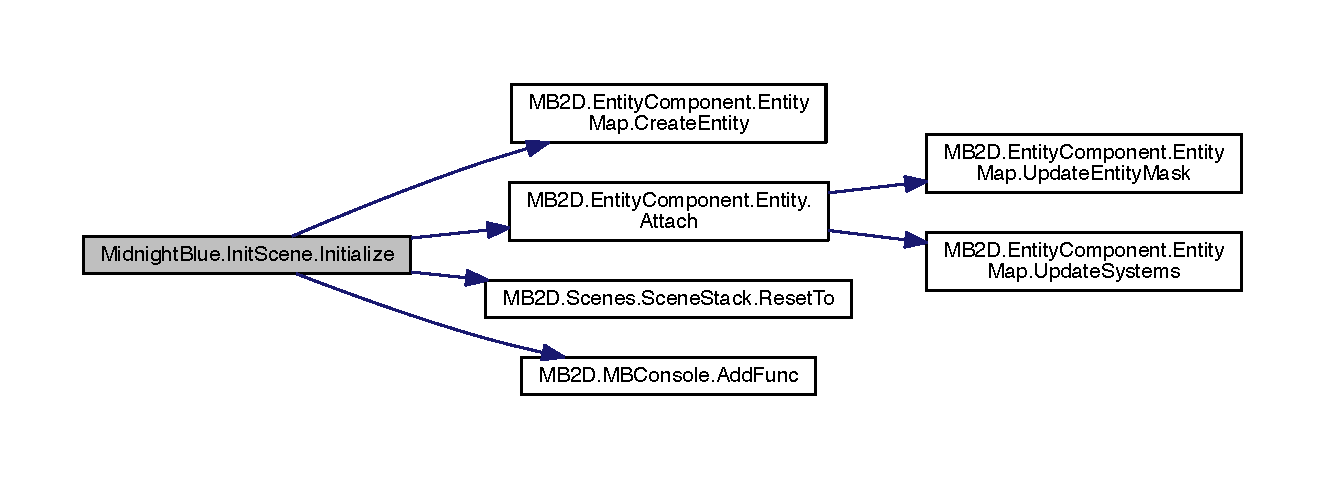
\includegraphics[width=350pt]{class_midnight_blue_1_1_init_scene_a99eee8cc5dab8d7263591aeaa50144fb_cgraph}
\end{center}
\end{figure}
\hypertarget{class_midnight_blue_1_1_init_scene_adbcab013e715e5c49ad09bcd0545d994}{}\label{class_midnight_blue_1_1_init_scene_adbcab013e715e5c49ad09bcd0545d994} 
\index{Midnight\+Blue\+::\+Init\+Scene@{Midnight\+Blue\+::\+Init\+Scene}!Pause@{Pause}}
\index{Pause@{Pause}!Midnight\+Blue\+::\+Init\+Scene@{Midnight\+Blue\+::\+Init\+Scene}}
\subsubsection{\texorpdfstring{Pause()}{Pause()}}
{\footnotesize\ttfamily override void Midnight\+Blue.\+Init\+Scene.\+Pause (\begin{DoxyParamCaption}{ }\end{DoxyParamCaption})\hspace{0.3cm}{\ttfamily [inline]}, {\ttfamily [virtual]}}



Pauses the scene. 



Implements \hyperlink{class_m_b2_d_1_1_scenes_1_1_scene_a0661eff0223150fa8e9ea88145409e5d}{M\+B2\+D.\+Scenes.\+Scene}.

\hypertarget{class_midnight_blue_1_1_init_scene_a01ade76252a492d20181bd2e00eb217f}{}\label{class_midnight_blue_1_1_init_scene_a01ade76252a492d20181bd2e00eb217f} 
\index{Midnight\+Blue\+::\+Init\+Scene@{Midnight\+Blue\+::\+Init\+Scene}!Resume@{Resume}}
\index{Resume@{Resume}!Midnight\+Blue\+::\+Init\+Scene@{Midnight\+Blue\+::\+Init\+Scene}}
\subsubsection{\texorpdfstring{Resume()}{Resume()}}
{\footnotesize\ttfamily override void Midnight\+Blue.\+Init\+Scene.\+Resume (\begin{DoxyParamCaption}{ }\end{DoxyParamCaption})\hspace{0.3cm}{\ttfamily [inline]}, {\ttfamily [virtual]}}



Resumes the scene. 



Implements \hyperlink{class_m_b2_d_1_1_scenes_1_1_scene_ad13639db22b059a1b714eefd9d927735}{M\+B2\+D.\+Scenes.\+Scene}.

Here is the call graph for this function\+:
\nopagebreak
\begin{figure}[H]
\begin{center}
\leavevmode
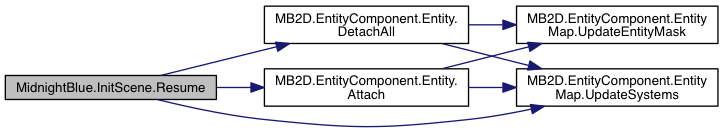
\includegraphics[width=350pt]{class_midnight_blue_1_1_init_scene_a01ade76252a492d20181bd2e00eb217f_cgraph}
\end{center}
\end{figure}
\hypertarget{class_midnight_blue_1_1_init_scene_ad87861fb4f2a30f5168f6133aa10d3f4}{}\label{class_midnight_blue_1_1_init_scene_ad87861fb4f2a30f5168f6133aa10d3f4} 
\index{Midnight\+Blue\+::\+Init\+Scene@{Midnight\+Blue\+::\+Init\+Scene}!Update@{Update}}
\index{Update@{Update}!Midnight\+Blue\+::\+Init\+Scene@{Midnight\+Blue\+::\+Init\+Scene}}
\subsubsection{\texorpdfstring{Update()}{Update()}}
{\footnotesize\ttfamily override void Midnight\+Blue.\+Init\+Scene.\+Update (\begin{DoxyParamCaption}{ }\end{DoxyParamCaption})\hspace{0.3cm}{\ttfamily [inline]}, {\ttfamily [virtual]}}



Updates the scene. 



Implements \hyperlink{class_m_b2_d_1_1_scenes_1_1_scene_a779de7c1ab23b698dcde3a228324a991}{M\+B2\+D.\+Scenes.\+Scene}.



The documentation for this class was generated from the following file\+:\begin{DoxyCompactItemize}
\item 
Shared/src/\+Game/\+Scenes/Init\+Scene.\+cs\end{DoxyCompactItemize}

\hypertarget{class_midnight_blue_1_1_land_command}{}\section{Midnight\+Blue.\+Land\+Command Class Reference}
\label{class_midnight_blue_1_1_land_command}\index{Midnight\+Blue.\+Land\+Command@{Midnight\+Blue.\+Land\+Command}}


Lands the ship  




Inheritance diagram for Midnight\+Blue.\+Land\+Command\+:
\nopagebreak
\begin{figure}[H]
\begin{center}
\leavevmode
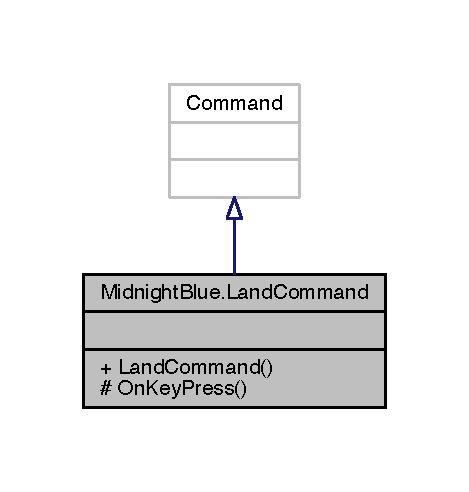
\includegraphics[width=225pt]{class_midnight_blue_1_1_land_command__inherit__graph}
\end{center}
\end{figure}


Collaboration diagram for Midnight\+Blue.\+Land\+Command\+:
\nopagebreak
\begin{figure}[H]
\begin{center}
\leavevmode
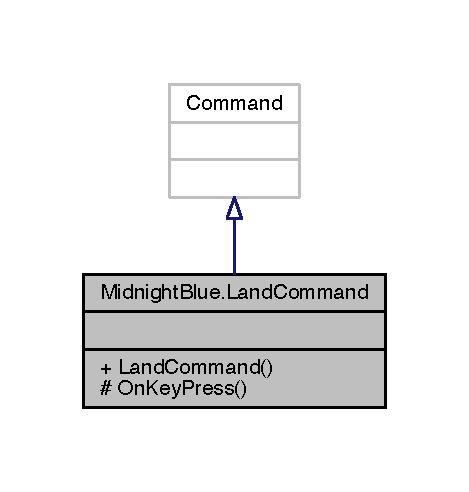
\includegraphics[width=225pt]{class_midnight_blue_1_1_land_command__coll__graph}
\end{center}
\end{figure}
\subsection*{Public Member Functions}
\begin{DoxyCompactItemize}
\item 
\hyperlink{class_midnight_blue_1_1_land_command_a936907822e22547099ec5267628fd457}{Land\+Command} (Keys key, Command\+Type type)
\begin{DoxyCompactList}\small\item\em Initializes a new instance of the T\+:\+Midnight\+Blue.\+Land\+Command class. \end{DoxyCompactList}\end{DoxyCompactItemize}
\subsection*{Protected Member Functions}
\begin{DoxyCompactItemize}
\item 
override void \hyperlink{class_midnight_blue_1_1_land_command_a2c496d96aed4498bb3ca133fcea4b172}{On\+Key\+Press} (Entity e)
\begin{DoxyCompactList}\small\item\em Lands the ship on the key press if terrain is landable \end{DoxyCompactList}\end{DoxyCompactItemize}


\subsection{Detailed Description}
Lands the ship 



\subsection{Constructor \& Destructor Documentation}
\hypertarget{class_midnight_blue_1_1_land_command_a936907822e22547099ec5267628fd457}{}\label{class_midnight_blue_1_1_land_command_a936907822e22547099ec5267628fd457} 
\index{Midnight\+Blue\+::\+Land\+Command@{Midnight\+Blue\+::\+Land\+Command}!Land\+Command@{Land\+Command}}
\index{Land\+Command@{Land\+Command}!Midnight\+Blue\+::\+Land\+Command@{Midnight\+Blue\+::\+Land\+Command}}
\subsubsection{\texorpdfstring{Land\+Command()}{LandCommand()}}
{\footnotesize\ttfamily Midnight\+Blue.\+Land\+Command.\+Land\+Command (\begin{DoxyParamCaption}\item[{Keys}]{key,  }\item[{Command\+Type}]{type }\end{DoxyParamCaption})\hspace{0.3cm}{\ttfamily [inline]}}



Initializes a new instance of the T\+:\+Midnight\+Blue.\+Land\+Command class. 


\begin{DoxyParams}{Parameters}
{\em key} & Key to assign to.\\
\hline
{\em type} & Trigger type.\\
\hline
\end{DoxyParams}


\subsection{Member Function Documentation}
\hypertarget{class_midnight_blue_1_1_land_command_a2c496d96aed4498bb3ca133fcea4b172}{}\label{class_midnight_blue_1_1_land_command_a2c496d96aed4498bb3ca133fcea4b172} 
\index{Midnight\+Blue\+::\+Land\+Command@{Midnight\+Blue\+::\+Land\+Command}!On\+Key\+Press@{On\+Key\+Press}}
\index{On\+Key\+Press@{On\+Key\+Press}!Midnight\+Blue\+::\+Land\+Command@{Midnight\+Blue\+::\+Land\+Command}}
\subsubsection{\texorpdfstring{On\+Key\+Press()}{OnKeyPress()}}
{\footnotesize\ttfamily override void Midnight\+Blue.\+Land\+Command.\+On\+Key\+Press (\begin{DoxyParamCaption}\item[{Entity}]{e }\end{DoxyParamCaption})\hspace{0.3cm}{\ttfamily [inline]}, {\ttfamily [protected]}}



Lands the ship on the key press if terrain is landable 


\begin{DoxyParams}{Parameters}
{\em e} & Entity with the ship controller to operate on.\\
\hline
\end{DoxyParams}


The documentation for this class was generated from the following file\+:\begin{DoxyCompactItemize}
\item 
Shared/src/\+Game/\+Commands/Ship\+Commands.\+cs\end{DoxyCompactItemize}

\hypertarget{class_midnight_blue_1_1_launch_command}{}\subsection{Midnight\+Blue.\+Launch\+Command Class Reference}
\label{class_midnight_blue_1_1_launch_command}\index{Midnight\+Blue.\+Launch\+Command@{Midnight\+Blue.\+Launch\+Command}}


Launches the ship from a landed state  




Inheritance diagram for Midnight\+Blue.\+Launch\+Command\+:\nopagebreak
\begin{figure}[H]
\begin{center}
\leavevmode
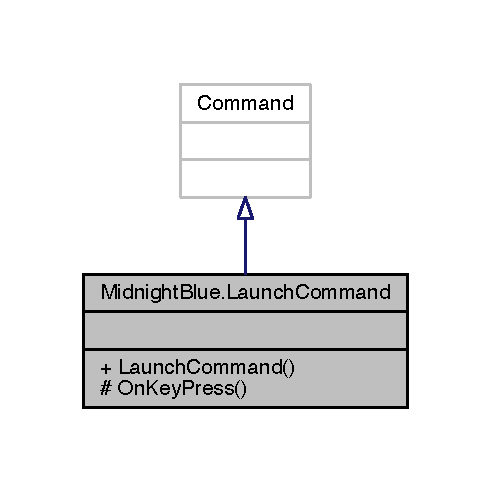
\includegraphics[width=236pt]{class_midnight_blue_1_1_launch_command__inherit__graph}
\end{center}
\end{figure}


Collaboration diagram for Midnight\+Blue.\+Launch\+Command\+:\nopagebreak
\begin{figure}[H]
\begin{center}
\leavevmode
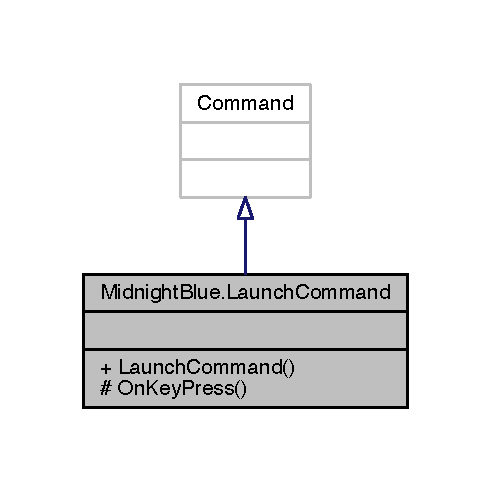
\includegraphics[width=236pt]{class_midnight_blue_1_1_launch_command__coll__graph}
\end{center}
\end{figure}
\subsubsection*{Public Member Functions}
\begin{DoxyCompactItemize}
\item 
\hyperlink{class_midnight_blue_1_1_launch_command_af557e1d21514b76f8adb28fd5c43d279}{Launch\+Command} (Keys key, Command\+Type type)
\begin{DoxyCompactList}\small\item\em Initializes a new instance of the T\+:\+Midnight\+Blue.\+Launch\+Command class. \end{DoxyCompactList}\end{DoxyCompactItemize}
\subsubsection*{Protected Member Functions}
\begin{DoxyCompactItemize}
\item 
override void \hyperlink{class_midnight_blue_1_1_launch_command_a5da2fdd898111ea59f4f63126c380a3e}{On\+Key\+Press} (Entity e)
\begin{DoxyCompactList}\small\item\em Launches the ship from landed on key press. \end{DoxyCompactList}\end{DoxyCompactItemize}


\subsubsection{Detailed Description}
Launches the ship from a landed state 



\subsubsection{Constructor \& Destructor Documentation}
\hypertarget{class_midnight_blue_1_1_launch_command_af557e1d21514b76f8adb28fd5c43d279}{}\label{class_midnight_blue_1_1_launch_command_af557e1d21514b76f8adb28fd5c43d279} 
\index{Midnight\+Blue\+::\+Launch\+Command@{Midnight\+Blue\+::\+Launch\+Command}!Launch\+Command@{Launch\+Command}}
\index{Launch\+Command@{Launch\+Command}!Midnight\+Blue\+::\+Launch\+Command@{Midnight\+Blue\+::\+Launch\+Command}}
\paragraph{\texorpdfstring{Launch\+Command()}{LaunchCommand()}}
{\footnotesize\ttfamily Midnight\+Blue.\+Launch\+Command.\+Launch\+Command (\begin{DoxyParamCaption}\item[{Keys}]{key,  }\item[{Command\+Type}]{type }\end{DoxyParamCaption})\hspace{0.3cm}{\ttfamily [inline]}}



Initializes a new instance of the T\+:\+Midnight\+Blue.\+Launch\+Command class. 


\begin{DoxyParams}{Parameters}
{\em key} & Key to assign to.\\
\hline
{\em type} & Trigger type.\\
\hline
\end{DoxyParams}


\subsubsection{Member Function Documentation}
\hypertarget{class_midnight_blue_1_1_launch_command_a5da2fdd898111ea59f4f63126c380a3e}{}\label{class_midnight_blue_1_1_launch_command_a5da2fdd898111ea59f4f63126c380a3e} 
\index{Midnight\+Blue\+::\+Launch\+Command@{Midnight\+Blue\+::\+Launch\+Command}!On\+Key\+Press@{On\+Key\+Press}}
\index{On\+Key\+Press@{On\+Key\+Press}!Midnight\+Blue\+::\+Launch\+Command@{Midnight\+Blue\+::\+Launch\+Command}}
\paragraph{\texorpdfstring{On\+Key\+Press()}{OnKeyPress()}}
{\footnotesize\ttfamily override void Midnight\+Blue.\+Launch\+Command.\+On\+Key\+Press (\begin{DoxyParamCaption}\item[{Entity}]{e }\end{DoxyParamCaption})\hspace{0.3cm}{\ttfamily [inline]}, {\ttfamily [protected]}}



Launches the ship from landed on key press. 


\begin{DoxyParams}{Parameters}
{\em e} & Entity with ship controller to operate on.\\
\hline
\end{DoxyParams}


The documentation for this class was generated from the following file\+:\begin{DoxyCompactItemize}
\item 
Shared/src/\+Game/\+Commands/Ship\+Commands.\+cs\end{DoxyCompactItemize}

\hypertarget{class_midnight_blue_1_1_leave_star_system}{}\section{Midnight\+Blue.\+Leave\+Star\+System Class Reference}
\label{class_midnight_blue_1_1_leave_star_system}\index{Midnight\+Blue.\+Leave\+Star\+System@{Midnight\+Blue.\+Leave\+Star\+System}}


Inheritance diagram for Midnight\+Blue.\+Leave\+Star\+System\+:\nopagebreak
\begin{figure}[H]
\begin{center}
\leavevmode
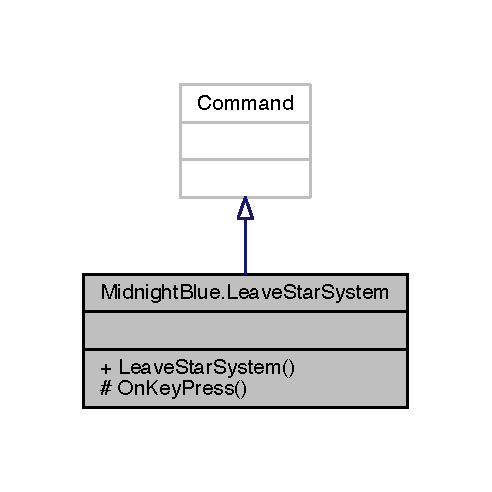
\includegraphics[width=236pt]{class_midnight_blue_1_1_leave_star_system__inherit__graph}
\end{center}
\end{figure}


Collaboration diagram for Midnight\+Blue.\+Leave\+Star\+System\+:\nopagebreak
\begin{figure}[H]
\begin{center}
\leavevmode
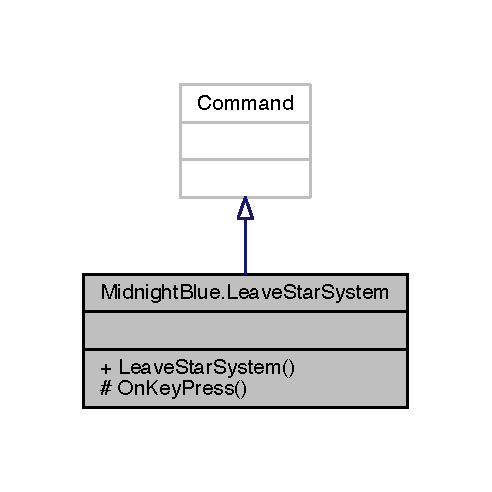
\includegraphics[width=236pt]{class_midnight_blue_1_1_leave_star_system__coll__graph}
\end{center}
\end{figure}
\subsection*{Public Member Functions}
\begin{DoxyCompactItemize}
\item 
\hyperlink{class_midnight_blue_1_1_leave_star_system_a6793d6a941afd58a9e9030d8aec1fe83}{Leave\+Star\+System} (Keys key, \hyperlink{namespace_m_b2_d_1_1_i_o_ab5f95f3fe9e652778b62bdf943168a68}{Command\+Type} type)
\begin{DoxyCompactList}\small\item\em Initializes a new instance of the T\+:\+Midnight\+Blue.\+Leave\+Star\+System class. \end{DoxyCompactList}\end{DoxyCompactItemize}
\subsection*{Protected Member Functions}
\begin{DoxyCompactItemize}
\item 
override void \hyperlink{class_midnight_blue_1_1_leave_star_system_ad2e048edbe7a4816d9ed8fc87cf4eb91}{On\+Key\+Press} (\hyperlink{class_m_b2_d_1_1_entity_component_1_1_entity}{Entity} e=null)
\begin{DoxyCompactList}\small\item\em Defines the logic to perform when operating on a given entity \end{DoxyCompactList}\end{DoxyCompactItemize}
\subsection*{Additional Inherited Members}


\subsection{Constructor \& Destructor Documentation}
\hypertarget{class_midnight_blue_1_1_leave_star_system_a6793d6a941afd58a9e9030d8aec1fe83}{}\label{class_midnight_blue_1_1_leave_star_system_a6793d6a941afd58a9e9030d8aec1fe83} 
\index{Midnight\+Blue\+::\+Leave\+Star\+System@{Midnight\+Blue\+::\+Leave\+Star\+System}!Leave\+Star\+System@{Leave\+Star\+System}}
\index{Leave\+Star\+System@{Leave\+Star\+System}!Midnight\+Blue\+::\+Leave\+Star\+System@{Midnight\+Blue\+::\+Leave\+Star\+System}}
\subsubsection{\texorpdfstring{Leave\+Star\+System()}{LeaveStarSystem()}}
{\footnotesize\ttfamily Midnight\+Blue.\+Leave\+Star\+System.\+Leave\+Star\+System (\begin{DoxyParamCaption}\item[{Keys}]{key,  }\item[{\hyperlink{namespace_m_b2_d_1_1_i_o_ab5f95f3fe9e652778b62bdf943168a68}{Command\+Type}}]{type }\end{DoxyParamCaption})\hspace{0.3cm}{\ttfamily [inline]}}



Initializes a new instance of the T\+:\+Midnight\+Blue.\+Leave\+Star\+System class. 


\begin{DoxyParams}{Parameters}
{\em key} & Key to assign to.\\
\hline
{\em type} & Trigger type.\\
\hline
\end{DoxyParams}


\subsection{Member Function Documentation}
\hypertarget{class_midnight_blue_1_1_leave_star_system_ad2e048edbe7a4816d9ed8fc87cf4eb91}{}\label{class_midnight_blue_1_1_leave_star_system_ad2e048edbe7a4816d9ed8fc87cf4eb91} 
\index{Midnight\+Blue\+::\+Leave\+Star\+System@{Midnight\+Blue\+::\+Leave\+Star\+System}!On\+Key\+Press@{On\+Key\+Press}}
\index{On\+Key\+Press@{On\+Key\+Press}!Midnight\+Blue\+::\+Leave\+Star\+System@{Midnight\+Blue\+::\+Leave\+Star\+System}}
\subsubsection{\texorpdfstring{On\+Key\+Press()}{OnKeyPress()}}
{\footnotesize\ttfamily override void Midnight\+Blue.\+Leave\+Star\+System.\+On\+Key\+Press (\begin{DoxyParamCaption}\item[{\hyperlink{class_m_b2_d_1_1_entity_component_1_1_entity}{Entity}}]{e = {\ttfamily null} }\end{DoxyParamCaption})\hspace{0.3cm}{\ttfamily [inline]}, {\ttfamily [protected]}, {\ttfamily [virtual]}}



Defines the logic to perform when operating on a given entity 


\begin{DoxyParams}{Parameters}
{\em e} & Entity to operate on\\
\hline
\end{DoxyParams}


Implements \hyperlink{class_m_b2_d_1_1_i_o_1_1_command_ae927e36c0e285848325cc68eddb5fd72}{M\+B2\+D.\+I\+O.\+Command}.



The documentation for this class was generated from the following file\+:\begin{DoxyCompactItemize}
\item 
Shared/src/\+Game/\+Commands/Ship\+Commands.\+cs\end{DoxyCompactItemize}

\hypertarget{class_midnight_blue_1_1_length}{}\section{Midnight\+Blue.\+Length Class Reference}
\label{class_midnight_blue_1_1_length}\index{Midnight\+Blue.\+Length@{Midnight\+Blue.\+Length}}


Defines a measurement of length in meters able to be converted to other measurements.  




Collaboration diagram for Midnight\+Blue.\+Length\+:\nopagebreak
\begin{figure}[H]
\begin{center}
\leavevmode
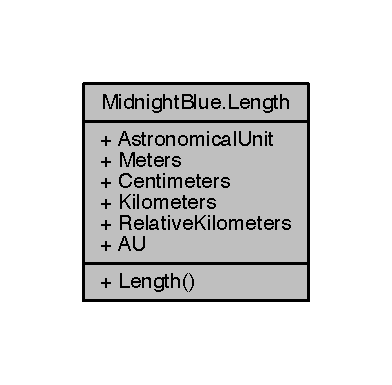
\includegraphics[width=188pt]{class_midnight_blue_1_1_length__coll__graph}
\end{center}
\end{figure}
\subsection*{Public Member Functions}
\begin{DoxyCompactItemize}
\item 
\hyperlink{class_midnight_blue_1_1_length_a8c58b161c6f730c22d84b01b078bd091}{Length} (ulong meters)
\begin{DoxyCompactList}\small\item\em Initializes a new instance of the T\+:\+Midnight\+Blue.\+Length class. \end{DoxyCompactList}\end{DoxyCompactItemize}
\subsection*{Public Attributes}
\begin{DoxyCompactItemize}
\item 
const float \hyperlink{class_midnight_blue_1_1_length_a5e86fa7e1d296ca9e6c5406a863427a6}{Astronomical\+Unit} = 149597870.\+7f
\begin{DoxyCompactList}\small\item\em A single Astronomical Unit in kilometers \end{DoxyCompactList}\end{DoxyCompactItemize}
\subsection*{Properties}
\begin{DoxyCompactItemize}
\item 
ulong \hyperlink{class_midnight_blue_1_1_length_ac824fa58d75ab754c33cdc8bfd49e5b0}{Meters}\hspace{0.3cm}{\ttfamily  \mbox{[}get\mbox{]}}
\begin{DoxyCompactList}\small\item\em Gets the length in meters \end{DoxyCompactList}\item 
ulong \hyperlink{class_midnight_blue_1_1_length_a935aac3abfc2865e5960a40382227063}{Centimeters}\hspace{0.3cm}{\ttfamily  \mbox{[}get\mbox{]}}
\begin{DoxyCompactList}\small\item\em Gets the length in centimeters \end{DoxyCompactList}\item 
ulong \hyperlink{class_midnight_blue_1_1_length_abf0d08eda94640cdb4706f96c3a97a29}{Kilometers}\hspace{0.3cm}{\ttfamily  \mbox{[}get\mbox{]}}
\begin{DoxyCompactList}\small\item\em Gets the length in kilometers \end{DoxyCompactList}\item 
int \hyperlink{class_midnight_blue_1_1_length_a7073632b5e2dfc836266de44378941be}{Relative\+Kilometers}\hspace{0.3cm}{\ttfamily  \mbox{[}get\mbox{]}}
\begin{DoxyCompactList}\small\item\em Gets the length in kilometers represented as a smaller value used for calculations. \end{DoxyCompactList}\item 
float \hyperlink{class_midnight_blue_1_1_length_aa2325bd4894b015715784b027551826f}{AU}\hspace{0.3cm}{\ttfamily  \mbox{[}get\mbox{]}}
\begin{DoxyCompactList}\small\item\em Gets the length in Astronomical Unites \end{DoxyCompactList}\end{DoxyCompactItemize}


\subsection{Detailed Description}
Defines a measurement of length in meters able to be converted to other measurements. 



\subsection{Constructor \& Destructor Documentation}
\hypertarget{class_midnight_blue_1_1_length_a8c58b161c6f730c22d84b01b078bd091}{}\label{class_midnight_blue_1_1_length_a8c58b161c6f730c22d84b01b078bd091} 
\index{Midnight\+Blue\+::\+Length@{Midnight\+Blue\+::\+Length}!Length@{Length}}
\index{Length@{Length}!Midnight\+Blue\+::\+Length@{Midnight\+Blue\+::\+Length}}
\subsubsection{\texorpdfstring{Length()}{Length()}}
{\footnotesize\ttfamily Midnight\+Blue.\+Length.\+Length (\begin{DoxyParamCaption}\item[{ulong}]{meters }\end{DoxyParamCaption})\hspace{0.3cm}{\ttfamily [inline]}}



Initializes a new instance of the T\+:\+Midnight\+Blue.\+Length class. 


\begin{DoxyParams}{Parameters}
{\em meters} & Initial length to set in meters.\\
\hline
\end{DoxyParams}


\subsection{Member Data Documentation}
\hypertarget{class_midnight_blue_1_1_length_a5e86fa7e1d296ca9e6c5406a863427a6}{}\label{class_midnight_blue_1_1_length_a5e86fa7e1d296ca9e6c5406a863427a6} 
\index{Midnight\+Blue\+::\+Length@{Midnight\+Blue\+::\+Length}!Astronomical\+Unit@{Astronomical\+Unit}}
\index{Astronomical\+Unit@{Astronomical\+Unit}!Midnight\+Blue\+::\+Length@{Midnight\+Blue\+::\+Length}}
\subsubsection{\texorpdfstring{Astronomical\+Unit}{AstronomicalUnit}}
{\footnotesize\ttfamily const float Midnight\+Blue.\+Length.\+Astronomical\+Unit = 149597870.\+7f}



A single Astronomical Unit in kilometers 



\subsection{Property Documentation}
\hypertarget{class_midnight_blue_1_1_length_aa2325bd4894b015715784b027551826f}{}\label{class_midnight_blue_1_1_length_aa2325bd4894b015715784b027551826f} 
\index{Midnight\+Blue\+::\+Length@{Midnight\+Blue\+::\+Length}!AU@{AU}}
\index{AU@{AU}!Midnight\+Blue\+::\+Length@{Midnight\+Blue\+::\+Length}}
\subsubsection{\texorpdfstring{AU}{AU}}
{\footnotesize\ttfamily float Midnight\+Blue.\+Length.\+AU\hspace{0.3cm}{\ttfamily [get]}}



Gets the length in Astronomical Unites 

The length in astronomical units.\hypertarget{class_midnight_blue_1_1_length_a935aac3abfc2865e5960a40382227063}{}\label{class_midnight_blue_1_1_length_a935aac3abfc2865e5960a40382227063} 
\index{Midnight\+Blue\+::\+Length@{Midnight\+Blue\+::\+Length}!Centimeters@{Centimeters}}
\index{Centimeters@{Centimeters}!Midnight\+Blue\+::\+Length@{Midnight\+Blue\+::\+Length}}
\subsubsection{\texorpdfstring{Centimeters}{Centimeters}}
{\footnotesize\ttfamily ulong Midnight\+Blue.\+Length.\+Centimeters\hspace{0.3cm}{\ttfamily [get]}}



Gets the length in centimeters 

The length in centimeters.\hypertarget{class_midnight_blue_1_1_length_abf0d08eda94640cdb4706f96c3a97a29}{}\label{class_midnight_blue_1_1_length_abf0d08eda94640cdb4706f96c3a97a29} 
\index{Midnight\+Blue\+::\+Length@{Midnight\+Blue\+::\+Length}!Kilometers@{Kilometers}}
\index{Kilometers@{Kilometers}!Midnight\+Blue\+::\+Length@{Midnight\+Blue\+::\+Length}}
\subsubsection{\texorpdfstring{Kilometers}{Kilometers}}
{\footnotesize\ttfamily ulong Midnight\+Blue.\+Length.\+Kilometers\hspace{0.3cm}{\ttfamily [get]}}



Gets the length in kilometers 

The length in kilometers.\hypertarget{class_midnight_blue_1_1_length_ac824fa58d75ab754c33cdc8bfd49e5b0}{}\label{class_midnight_blue_1_1_length_ac824fa58d75ab754c33cdc8bfd49e5b0} 
\index{Midnight\+Blue\+::\+Length@{Midnight\+Blue\+::\+Length}!Meters@{Meters}}
\index{Meters@{Meters}!Midnight\+Blue\+::\+Length@{Midnight\+Blue\+::\+Length}}
\subsubsection{\texorpdfstring{Meters}{Meters}}
{\footnotesize\ttfamily ulong Midnight\+Blue.\+Length.\+Meters\hspace{0.3cm}{\ttfamily [get]}}



Gets the length in meters 

The length in meters.\hypertarget{class_midnight_blue_1_1_length_a7073632b5e2dfc836266de44378941be}{}\label{class_midnight_blue_1_1_length_a7073632b5e2dfc836266de44378941be} 
\index{Midnight\+Blue\+::\+Length@{Midnight\+Blue\+::\+Length}!Relative\+Kilometers@{Relative\+Kilometers}}
\index{Relative\+Kilometers@{Relative\+Kilometers}!Midnight\+Blue\+::\+Length@{Midnight\+Blue\+::\+Length}}
\subsubsection{\texorpdfstring{Relative\+Kilometers}{RelativeKilometers}}
{\footnotesize\ttfamily int Midnight\+Blue.\+Length.\+Relative\+Kilometers\hspace{0.3cm}{\ttfamily [get]}}



Gets the length in kilometers represented as a smaller value used for calculations. 

The length in relative kilometers.

The documentation for this class was generated from the following file\+:\begin{DoxyCompactItemize}
\item 
Shared/src/\+Game/\+Environment/Length.\+cs\end{DoxyCompactItemize}

\hypertarget{class_midnight_blue_1_1_testing_1_1_map_test}{}\section{Midnight\+Blue.\+Testing.\+Map\+Test Class Reference}
\label{class_midnight_blue_1_1_testing_1_1_map_test}\index{Midnight\+Blue.\+Testing.\+Map\+Test@{Midnight\+Blue.\+Testing.\+Map\+Test}}


Inheritance diagram for Midnight\+Blue.\+Testing.\+Map\+Test\+:
\nopagebreak
\begin{figure}[H]
\begin{center}
\leavevmode
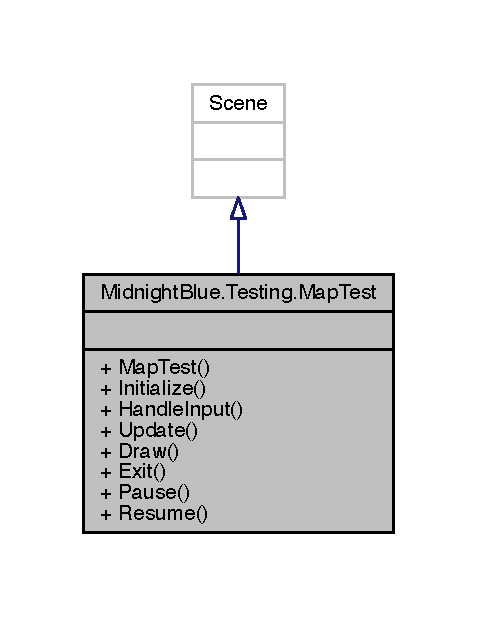
\includegraphics[width=229pt]{class_midnight_blue_1_1_testing_1_1_map_test__inherit__graph}
\end{center}
\end{figure}


Collaboration diagram for Midnight\+Blue.\+Testing.\+Map\+Test\+:
\nopagebreak
\begin{figure}[H]
\begin{center}
\leavevmode
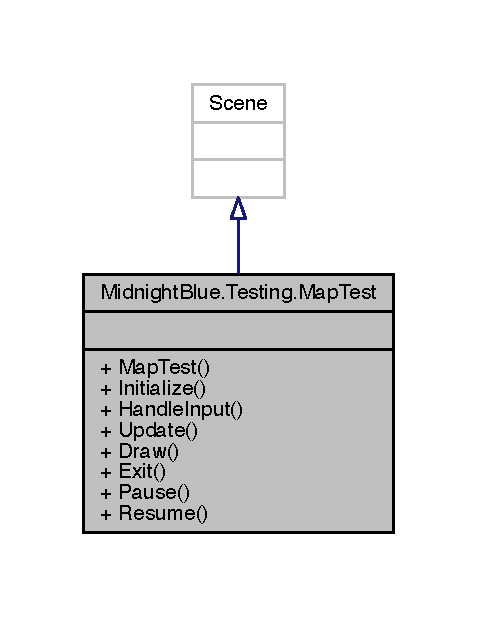
\includegraphics[width=229pt]{class_midnight_blue_1_1_testing_1_1_map_test__coll__graph}
\end{center}
\end{figure}
\subsection*{Public Member Functions}
\begin{DoxyCompactItemize}
\item 
\hypertarget{class_midnight_blue_1_1_testing_1_1_map_test_a7fb98572efcce64a85eaec1363fdddd4}{}\label{class_midnight_blue_1_1_testing_1_1_map_test_a7fb98572efcce64a85eaec1363fdddd4} 
{\bfseries Map\+Test} (Entity\+Map map, Content\+Manager content)
\item 
\hypertarget{class_midnight_blue_1_1_testing_1_1_map_test_adcaa2f37efbf5764b48d297cabf17784}{}\label{class_midnight_blue_1_1_testing_1_1_map_test_adcaa2f37efbf5764b48d297cabf17784} 
override void {\bfseries Initialize} ()
\item 
\hypertarget{class_midnight_blue_1_1_testing_1_1_map_test_ad7e54e4aec415ccf6e89ce8a8876d259}{}\label{class_midnight_blue_1_1_testing_1_1_map_test_ad7e54e4aec415ccf6e89ce8a8876d259} 
override void {\bfseries Handle\+Input} ()
\item 
\hypertarget{class_midnight_blue_1_1_testing_1_1_map_test_ae4bb817dd9c5b55bd1d818de9f527c7c}{}\label{class_midnight_blue_1_1_testing_1_1_map_test_ae4bb817dd9c5b55bd1d818de9f527c7c} 
override void {\bfseries Update} ()
\item 
\hypertarget{class_midnight_blue_1_1_testing_1_1_map_test_a03d0a9349662afafaa301a8581fbf01f}{}\label{class_midnight_blue_1_1_testing_1_1_map_test_a03d0a9349662afafaa301a8581fbf01f} 
override void {\bfseries Draw} (Sprite\+Batch sprite\+Batch, Sprite\+Batch ui\+Sprite\+Batch)
\item 
\hypertarget{class_midnight_blue_1_1_testing_1_1_map_test_a7dfcf609b9fd898f377297a0075d2159}{}\label{class_midnight_blue_1_1_testing_1_1_map_test_a7dfcf609b9fd898f377297a0075d2159} 
override void {\bfseries Exit} ()
\item 
\hypertarget{class_midnight_blue_1_1_testing_1_1_map_test_a7dba960137d634b15e4f4b7b3a86489f}{}\label{class_midnight_blue_1_1_testing_1_1_map_test_a7dba960137d634b15e4f4b7b3a86489f} 
override void {\bfseries Pause} ()
\item 
\hypertarget{class_midnight_blue_1_1_testing_1_1_map_test_aa595402e6d3702119877721f7cb3ab9f}{}\label{class_midnight_blue_1_1_testing_1_1_map_test_aa595402e6d3702119877721f7cb3ab9f} 
override void {\bfseries Resume} ()
\end{DoxyCompactItemize}


The documentation for this class was generated from the following file\+:\begin{DoxyCompactItemize}
\item 
Shared/src/\+Game/\+Tests/Map\+Test.\+cs\end{DoxyCompactItemize}

\hypertarget{class_midnight_blue_1_1_menu_command}{}\section{Midnight\+Blue.\+Menu\+Command Class Reference}
\label{class_midnight_blue_1_1_menu_command}\index{Midnight\+Blue.\+Menu\+Command@{Midnight\+Blue.\+Menu\+Command}}


Inheritance diagram for Midnight\+Blue.\+Menu\+Command\+:\nopagebreak
\begin{figure}[H]
\begin{center}
\leavevmode
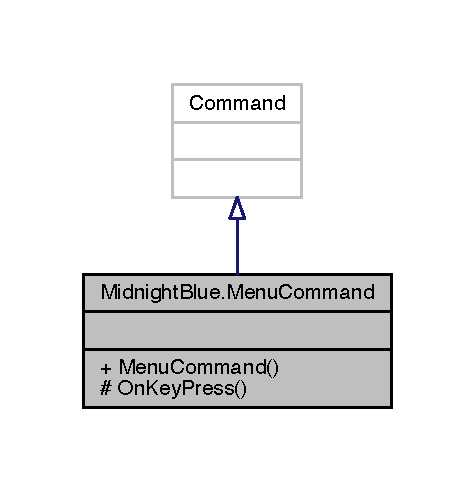
\includegraphics[width=228pt]{class_midnight_blue_1_1_menu_command__inherit__graph}
\end{center}
\end{figure}


Collaboration diagram for Midnight\+Blue.\+Menu\+Command\+:\nopagebreak
\begin{figure}[H]
\begin{center}
\leavevmode
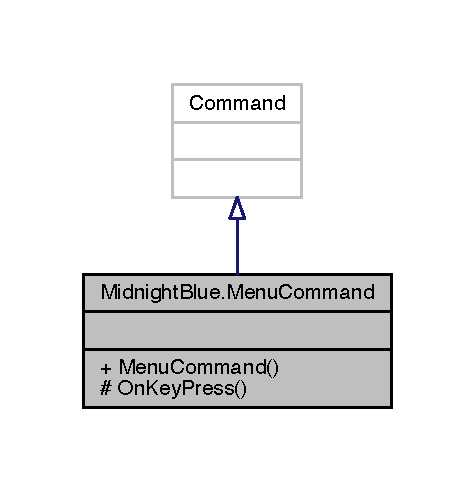
\includegraphics[width=228pt]{class_midnight_blue_1_1_menu_command__coll__graph}
\end{center}
\end{figure}
\subsection*{Public Member Functions}
\begin{DoxyCompactItemize}
\item 
\hypertarget{class_midnight_blue_1_1_menu_command_ac494139f6aafe9e9d1f24b3cce518279}{}\label{class_midnight_blue_1_1_menu_command_ac494139f6aafe9e9d1f24b3cce518279} 
{\bfseries Menu\+Command} (Keys key, \hyperlink{namespace_m_b2_d_1_1_i_o_ab5f95f3fe9e652778b62bdf943168a68}{Command\+Type} command\+Type, \hyperlink{class_m_b2_d_1_1_scenes_1_1_scene_stack}{Scene\+Stack} scene\+Controller, Content\+Manager content)
\end{DoxyCompactItemize}
\subsection*{Protected Member Functions}
\begin{DoxyCompactItemize}
\item 
override void \hyperlink{class_midnight_blue_1_1_menu_command_a2101f922aa12bd7fed4eff3eb714a9d4}{On\+Key\+Press} (\hyperlink{class_m_b2_d_1_1_entity_component_1_1_entity}{Entity} e=null)
\begin{DoxyCompactList}\small\item\em Defines the logic to perform when operating on a given entity \end{DoxyCompactList}\end{DoxyCompactItemize}
\subsection*{Additional Inherited Members}


\subsection{Member Function Documentation}
\hypertarget{class_midnight_blue_1_1_menu_command_a2101f922aa12bd7fed4eff3eb714a9d4}{}\label{class_midnight_blue_1_1_menu_command_a2101f922aa12bd7fed4eff3eb714a9d4} 
\index{Midnight\+Blue\+::\+Menu\+Command@{Midnight\+Blue\+::\+Menu\+Command}!On\+Key\+Press@{On\+Key\+Press}}
\index{On\+Key\+Press@{On\+Key\+Press}!Midnight\+Blue\+::\+Menu\+Command@{Midnight\+Blue\+::\+Menu\+Command}}
\subsubsection{\texorpdfstring{On\+Key\+Press()}{OnKeyPress()}}
{\footnotesize\ttfamily override void Midnight\+Blue.\+Menu\+Command.\+On\+Key\+Press (\begin{DoxyParamCaption}\item[{\hyperlink{class_m_b2_d_1_1_entity_component_1_1_entity}{Entity}}]{e = {\ttfamily null} }\end{DoxyParamCaption})\hspace{0.3cm}{\ttfamily [inline]}, {\ttfamily [protected]}, {\ttfamily [virtual]}}



Defines the logic to perform when operating on a given entity 


\begin{DoxyParams}{Parameters}
{\em e} & Entity to operate on\\
\hline
\end{DoxyParams}


Implements \hyperlink{class_m_b2_d_1_1_i_o_1_1_command_ae927e36c0e285848325cc68eddb5fd72}{M\+B2\+D.\+I\+O.\+Command}.

Here is the call graph for this function\+:\nopagebreak
\begin{figure}[H]
\begin{center}
\leavevmode
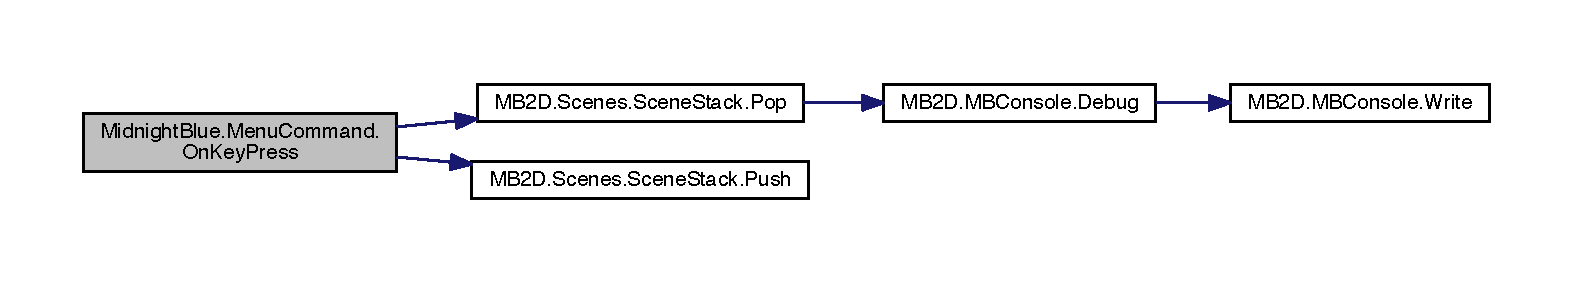
\includegraphics[width=350pt]{class_midnight_blue_1_1_menu_command_a2101f922aa12bd7fed4eff3eb714a9d4_cgraph}
\end{center}
\end{figure}


The documentation for this class was generated from the following file\+:\begin{DoxyCompactItemize}
\item 
Shared/src/\+Game/\+Commands/Menu\+Command.\+cs\end{DoxyCompactItemize}

\hypertarget{class_midnight_blue_1_1_menu_scene}{}\section{Midnight\+Blue.\+Menu\+Scene Class Reference}
\label{class_midnight_blue_1_1_menu_scene}\index{Midnight\+Blue.\+Menu\+Scene@{Midnight\+Blue.\+Menu\+Scene}}


Inheritance diagram for Midnight\+Blue.\+Menu\+Scene\+:
\nopagebreak
\begin{figure}[H]
\begin{center}
\leavevmode
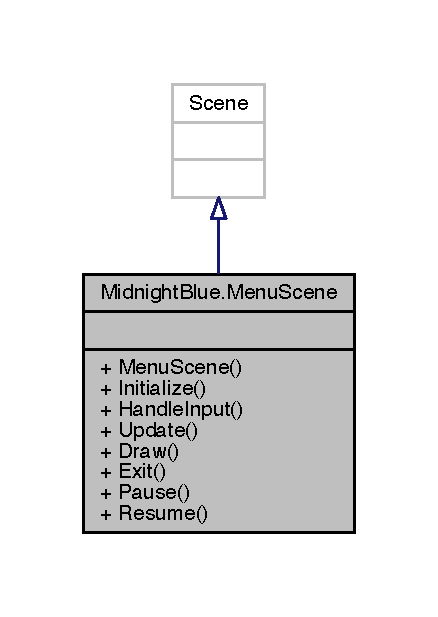
\includegraphics[width=217pt]{class_midnight_blue_1_1_menu_scene__inherit__graph}
\end{center}
\end{figure}


Collaboration diagram for Midnight\+Blue.\+Menu\+Scene\+:
\nopagebreak
\begin{figure}[H]
\begin{center}
\leavevmode
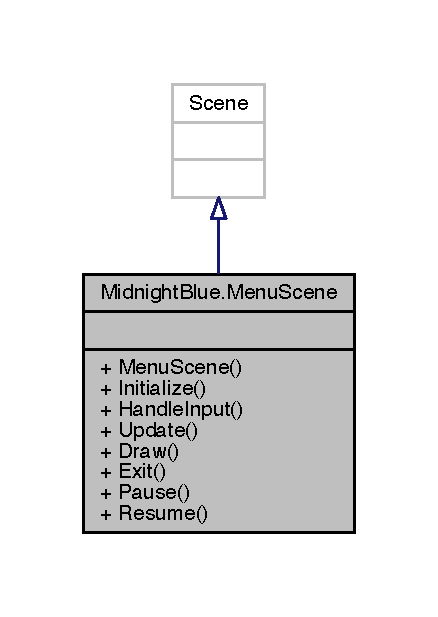
\includegraphics[width=217pt]{class_midnight_blue_1_1_menu_scene__coll__graph}
\end{center}
\end{figure}
\subsection*{Public Member Functions}
\begin{DoxyCompactItemize}
\item 
\hypertarget{class_midnight_blue_1_1_menu_scene_a7f0035320ea63bd527efcdbda32d3f2b}{}\label{class_midnight_blue_1_1_menu_scene_a7f0035320ea63bd527efcdbda32d3f2b} 
{\bfseries Menu\+Scene} (Content\+Manager content)
\item 
override void \hyperlink{class_midnight_blue_1_1_menu_scene_ab46d90617acf2fad0a3c759337c54aaf}{Initialize} ()
\begin{DoxyCompactList}\small\item\em Creates the U\+I\+View and starts the background music. \end{DoxyCompactList}\item 
override void \hyperlink{class_midnight_blue_1_1_menu_scene_a34d30a2b66e9eadbf0889071bca6fa57}{Handle\+Input} ()
\begin{DoxyCompactList}\small\item\em Handles the input for the menu. \end{DoxyCompactList}\item 
override void \hyperlink{class_midnight_blue_1_1_menu_scene_af82ad49ba2744422e52fc6c1b8544255}{Update} ()
\begin{DoxyCompactList}\small\item\em Updates the UI \end{DoxyCompactList}\item 
override void \hyperlink{class_midnight_blue_1_1_menu_scene_a600112073f48c763a50c802960f5fdaa}{Draw} (Sprite\+Batch sprite\+Batch, Sprite\+Batch ui\+Sprite\+Batch)
\begin{DoxyCompactList}\small\item\em Draws the UI to the ui\+Sprite\+Batch \end{DoxyCompactList}\item 
override void \hyperlink{class_midnight_blue_1_1_menu_scene_acc60288dc2dff4d612b7a63615165de5}{Exit} ()
\begin{DoxyCompactList}\small\item\em Exits the menu \end{DoxyCompactList}\item 
override void \hyperlink{class_midnight_blue_1_1_menu_scene_a7a2f8875f949d2ec2e6f3a8c6da7cedf}{Pause} ()
\begin{DoxyCompactList}\small\item\em Pauses the scene \end{DoxyCompactList}\item 
override void \hyperlink{class_midnight_blue_1_1_menu_scene_a76f8bd3add4abf16ac9962a2fb51fad2}{Resume} ()
\begin{DoxyCompactList}\small\item\em Resumes the scene \end{DoxyCompactList}\end{DoxyCompactItemize}
\subsection*{Additional Inherited Members}


\subsection{Member Function Documentation}
\hypertarget{class_midnight_blue_1_1_menu_scene_a600112073f48c763a50c802960f5fdaa}{}\label{class_midnight_blue_1_1_menu_scene_a600112073f48c763a50c802960f5fdaa} 
\index{Midnight\+Blue\+::\+Menu\+Scene@{Midnight\+Blue\+::\+Menu\+Scene}!Draw@{Draw}}
\index{Draw@{Draw}!Midnight\+Blue\+::\+Menu\+Scene@{Midnight\+Blue\+::\+Menu\+Scene}}
\subsubsection{\texorpdfstring{Draw()}{Draw()}}
{\footnotesize\ttfamily override void Midnight\+Blue.\+Menu\+Scene.\+Draw (\begin{DoxyParamCaption}\item[{Sprite\+Batch}]{sprite\+Batch,  }\item[{Sprite\+Batch}]{ui\+Sprite\+Batch }\end{DoxyParamCaption})\hspace{0.3cm}{\ttfamily [inline]}, {\ttfamily [virtual]}}



Draws the UI to the ui\+Sprite\+Batch 


\begin{DoxyParams}{Parameters}
{\em sprite\+Batch} & Sprite batch for world-\/based entities.\\
\hline
{\em ui\+Sprite\+Batch} & User interface sprite batch.\\
\hline
\end{DoxyParams}


Implements \hyperlink{class_m_b2_d_1_1_scenes_1_1_scene_a932d33071ecb4c5187367825dba72324}{M\+B2\+D.\+Scenes.\+Scene}.

Here is the call graph for this function\+:
\nopagebreak
\begin{figure}[H]
\begin{center}
\leavevmode
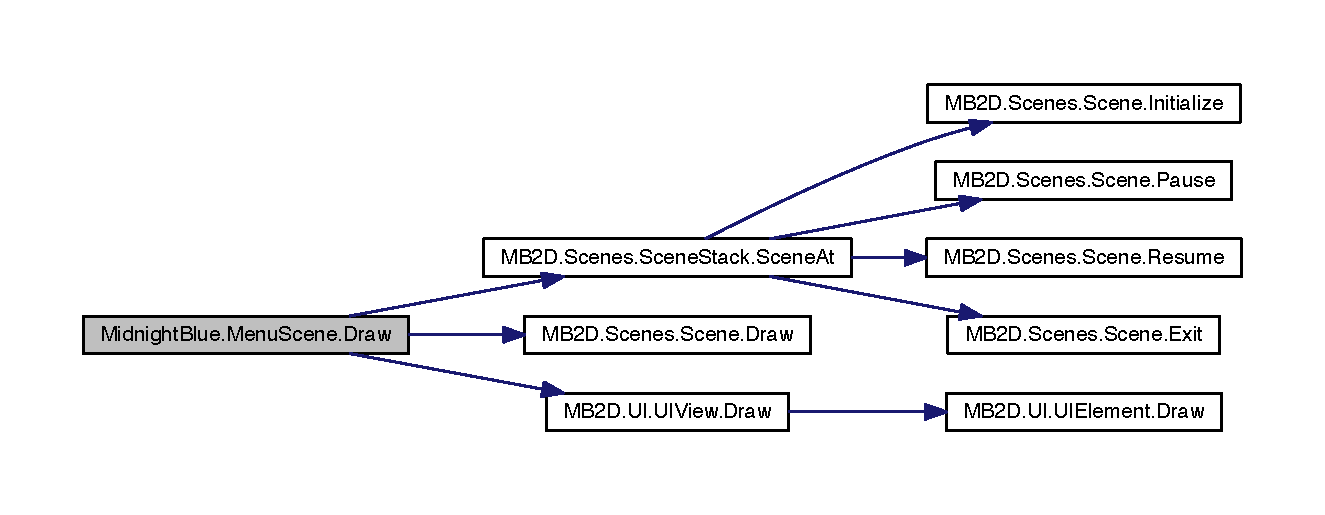
\includegraphics[width=350pt]{class_midnight_blue_1_1_menu_scene_a600112073f48c763a50c802960f5fdaa_cgraph}
\end{center}
\end{figure}
\hypertarget{class_midnight_blue_1_1_menu_scene_acc60288dc2dff4d612b7a63615165de5}{}\label{class_midnight_blue_1_1_menu_scene_acc60288dc2dff4d612b7a63615165de5} 
\index{Midnight\+Blue\+::\+Menu\+Scene@{Midnight\+Blue\+::\+Menu\+Scene}!Exit@{Exit}}
\index{Exit@{Exit}!Midnight\+Blue\+::\+Menu\+Scene@{Midnight\+Blue\+::\+Menu\+Scene}}
\subsubsection{\texorpdfstring{Exit()}{Exit()}}
{\footnotesize\ttfamily override void Midnight\+Blue.\+Menu\+Scene.\+Exit (\begin{DoxyParamCaption}{ }\end{DoxyParamCaption})\hspace{0.3cm}{\ttfamily [inline]}, {\ttfamily [virtual]}}



Exits the menu 



Implements \hyperlink{class_m_b2_d_1_1_scenes_1_1_scene_a099b79e16d23b67349847999d2336813}{M\+B2\+D.\+Scenes.\+Scene}.

\hypertarget{class_midnight_blue_1_1_menu_scene_a34d30a2b66e9eadbf0889071bca6fa57}{}\label{class_midnight_blue_1_1_menu_scene_a34d30a2b66e9eadbf0889071bca6fa57} 
\index{Midnight\+Blue\+::\+Menu\+Scene@{Midnight\+Blue\+::\+Menu\+Scene}!Handle\+Input@{Handle\+Input}}
\index{Handle\+Input@{Handle\+Input}!Midnight\+Blue\+::\+Menu\+Scene@{Midnight\+Blue\+::\+Menu\+Scene}}
\subsubsection{\texorpdfstring{Handle\+Input()}{HandleInput()}}
{\footnotesize\ttfamily override void Midnight\+Blue.\+Menu\+Scene.\+Handle\+Input (\begin{DoxyParamCaption}{ }\end{DoxyParamCaption})\hspace{0.3cm}{\ttfamily [inline]}, {\ttfamily [virtual]}}



Handles the input for the menu. 



Implements \hyperlink{class_m_b2_d_1_1_scenes_1_1_scene_a476de5a885408d27ff151044d20738c8}{M\+B2\+D.\+Scenes.\+Scene}.

\hypertarget{class_midnight_blue_1_1_menu_scene_ab46d90617acf2fad0a3c759337c54aaf}{}\label{class_midnight_blue_1_1_menu_scene_ab46d90617acf2fad0a3c759337c54aaf} 
\index{Midnight\+Blue\+::\+Menu\+Scene@{Midnight\+Blue\+::\+Menu\+Scene}!Initialize@{Initialize}}
\index{Initialize@{Initialize}!Midnight\+Blue\+::\+Menu\+Scene@{Midnight\+Blue\+::\+Menu\+Scene}}
\subsubsection{\texorpdfstring{Initialize()}{Initialize()}}
{\footnotesize\ttfamily override void Midnight\+Blue.\+Menu\+Scene.\+Initialize (\begin{DoxyParamCaption}{ }\end{DoxyParamCaption})\hspace{0.3cm}{\ttfamily [inline]}, {\ttfamily [virtual]}}



Creates the U\+I\+View and starts the background music. 



Implements \hyperlink{class_m_b2_d_1_1_scenes_1_1_scene_a081b4f8866936b495bdce388a7c96c25}{M\+B2\+D.\+Scenes.\+Scene}.

\hypertarget{class_midnight_blue_1_1_menu_scene_a7a2f8875f949d2ec2e6f3a8c6da7cedf}{}\label{class_midnight_blue_1_1_menu_scene_a7a2f8875f949d2ec2e6f3a8c6da7cedf} 
\index{Midnight\+Blue\+::\+Menu\+Scene@{Midnight\+Blue\+::\+Menu\+Scene}!Pause@{Pause}}
\index{Pause@{Pause}!Midnight\+Blue\+::\+Menu\+Scene@{Midnight\+Blue\+::\+Menu\+Scene}}
\subsubsection{\texorpdfstring{Pause()}{Pause()}}
{\footnotesize\ttfamily override void Midnight\+Blue.\+Menu\+Scene.\+Pause (\begin{DoxyParamCaption}{ }\end{DoxyParamCaption})\hspace{0.3cm}{\ttfamily [inline]}, {\ttfamily [virtual]}}



Pauses the scene 



Implements \hyperlink{class_m_b2_d_1_1_scenes_1_1_scene_a0661eff0223150fa8e9ea88145409e5d}{M\+B2\+D.\+Scenes.\+Scene}.

\hypertarget{class_midnight_blue_1_1_menu_scene_a76f8bd3add4abf16ac9962a2fb51fad2}{}\label{class_midnight_blue_1_1_menu_scene_a76f8bd3add4abf16ac9962a2fb51fad2} 
\index{Midnight\+Blue\+::\+Menu\+Scene@{Midnight\+Blue\+::\+Menu\+Scene}!Resume@{Resume}}
\index{Resume@{Resume}!Midnight\+Blue\+::\+Menu\+Scene@{Midnight\+Blue\+::\+Menu\+Scene}}
\subsubsection{\texorpdfstring{Resume()}{Resume()}}
{\footnotesize\ttfamily override void Midnight\+Blue.\+Menu\+Scene.\+Resume (\begin{DoxyParamCaption}{ }\end{DoxyParamCaption})\hspace{0.3cm}{\ttfamily [inline]}, {\ttfamily [virtual]}}



Resumes the scene 



Implements \hyperlink{class_m_b2_d_1_1_scenes_1_1_scene_ad13639db22b059a1b714eefd9d927735}{M\+B2\+D.\+Scenes.\+Scene}.

\hypertarget{class_midnight_blue_1_1_menu_scene_af82ad49ba2744422e52fc6c1b8544255}{}\label{class_midnight_blue_1_1_menu_scene_af82ad49ba2744422e52fc6c1b8544255} 
\index{Midnight\+Blue\+::\+Menu\+Scene@{Midnight\+Blue\+::\+Menu\+Scene}!Update@{Update}}
\index{Update@{Update}!Midnight\+Blue\+::\+Menu\+Scene@{Midnight\+Blue\+::\+Menu\+Scene}}
\subsubsection{\texorpdfstring{Update()}{Update()}}
{\footnotesize\ttfamily override void Midnight\+Blue.\+Menu\+Scene.\+Update (\begin{DoxyParamCaption}{ }\end{DoxyParamCaption})\hspace{0.3cm}{\ttfamily [inline]}, {\ttfamily [virtual]}}



Updates the UI 



Implements \hyperlink{class_m_b2_d_1_1_scenes_1_1_scene_a779de7c1ab23b698dcde3a228324a991}{M\+B2\+D.\+Scenes.\+Scene}.

Here is the call graph for this function\+:
\nopagebreak
\begin{figure}[H]
\begin{center}
\leavevmode
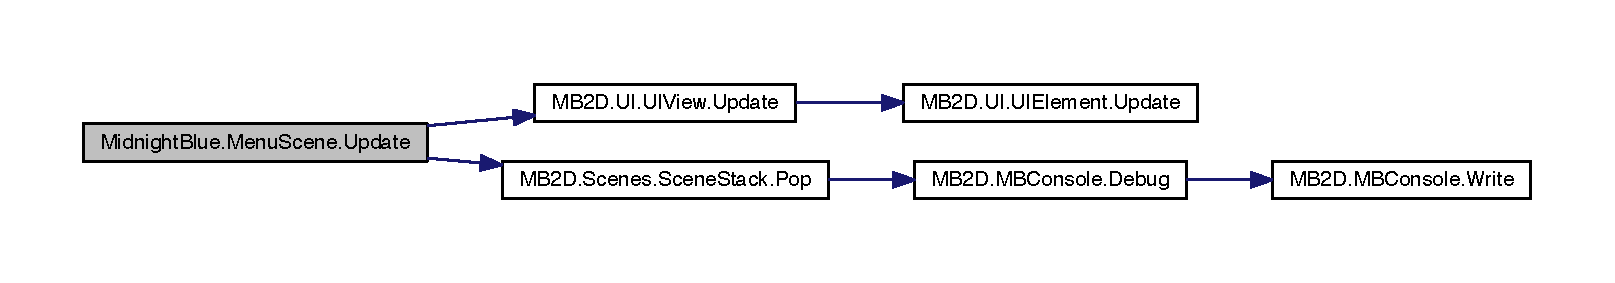
\includegraphics[width=350pt]{class_midnight_blue_1_1_menu_scene_af82ad49ba2744422e52fc6c1b8544255_cgraph}
\end{center}
\end{figure}


The documentation for this class was generated from the following file\+:\begin{DoxyCompactItemize}
\item 
Shared/src/\+Game/\+Scenes/Menu\+Scene.\+cs\end{DoxyCompactItemize}

\hypertarget{class_midnight_blue_1_1_menu_view}{}\section{Midnight\+Blue.\+Menu\+View Class Reference}
\label{class_midnight_blue_1_1_menu_view}\index{Midnight\+Blue.\+Menu\+View@{Midnight\+Blue.\+Menu\+View}}


Inheritance diagram for Midnight\+Blue.\+Menu\+View\+:\nopagebreak
\begin{figure}[H]
\begin{center}
\leavevmode
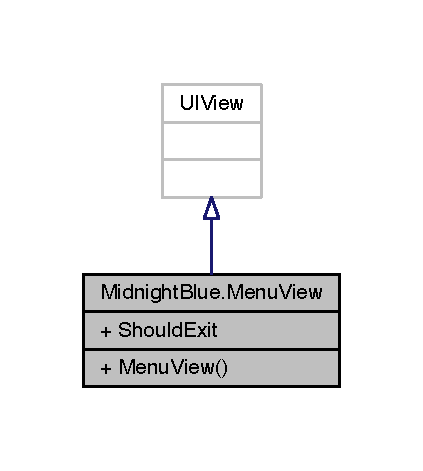
\includegraphics[width=203pt]{class_midnight_blue_1_1_menu_view__inherit__graph}
\end{center}
\end{figure}


Collaboration diagram for Midnight\+Blue.\+Menu\+View\+:\nopagebreak
\begin{figure}[H]
\begin{center}
\leavevmode
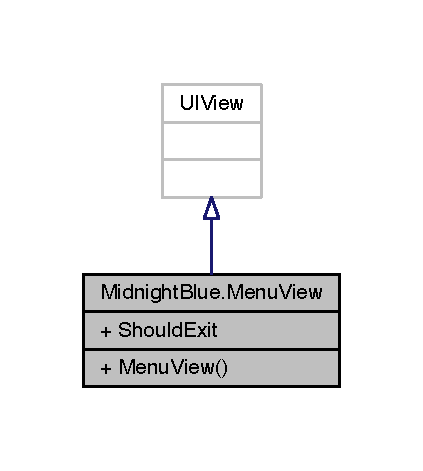
\includegraphics[width=203pt]{class_midnight_blue_1_1_menu_view__coll__graph}
\end{center}
\end{figure}
\subsection*{Public Member Functions}
\begin{DoxyCompactItemize}
\item 
\hypertarget{class_midnight_blue_1_1_menu_view_a80f778b2634f4b660f7f5e0393271a06}{}\label{class_midnight_blue_1_1_menu_view_a80f778b2634f4b660f7f5e0393271a06} 
{\bfseries Menu\+View} (Content\+Manager content)
\end{DoxyCompactItemize}
\subsection*{Properties}
\begin{DoxyCompactItemize}
\item 
\hypertarget{class_midnight_blue_1_1_menu_view_a8d81609074b935a6af5d9ac4238a73ee}{}\label{class_midnight_blue_1_1_menu_view_a8d81609074b935a6af5d9ac4238a73ee} 
bool {\bfseries Should\+Exit}\hspace{0.3cm}{\ttfamily  \mbox{[}get\mbox{]}}
\end{DoxyCompactItemize}


The documentation for this class was generated from the following file\+:\begin{DoxyCompactItemize}
\item 
Shared/src/\+Game/\+U\+I\+Views/Menu\+View.\+cs\end{DoxyCompactItemize}

\hypertarget{class_midnight_blue_1_1_move_ship}{}\section{Midnight\+Blue.\+Move\+Ship Class Reference}
\label{class_midnight_blue_1_1_move_ship}\index{Midnight\+Blue.\+Move\+Ship@{Midnight\+Blue.\+Move\+Ship}}


Performs logic aside from movement required to execute when moving the ship such as consuming fuel.  




Inheritance diagram for Midnight\+Blue.\+Move\+Ship\+:\nopagebreak
\begin{figure}[H]
\begin{center}
\leavevmode
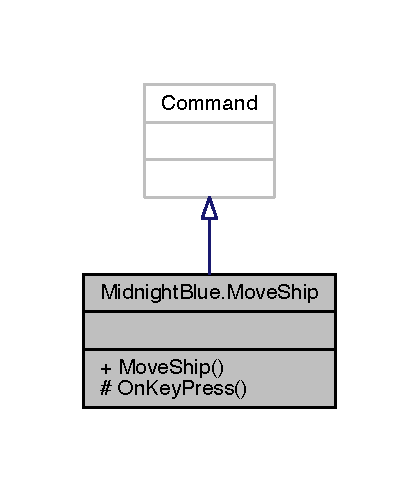
\includegraphics[width=201pt]{class_midnight_blue_1_1_move_ship__inherit__graph}
\end{center}
\end{figure}


Collaboration diagram for Midnight\+Blue.\+Move\+Ship\+:\nopagebreak
\begin{figure}[H]
\begin{center}
\leavevmode
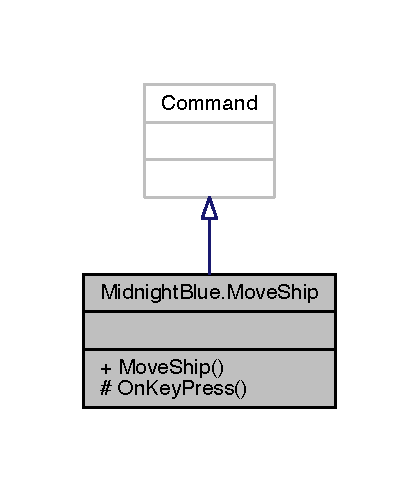
\includegraphics[width=201pt]{class_midnight_blue_1_1_move_ship__coll__graph}
\end{center}
\end{figure}
\subsection*{Public Member Functions}
\begin{DoxyCompactItemize}
\item 
\hyperlink{class_midnight_blue_1_1_move_ship_a7c3de7f43d19cde694040c71a5ee5fa0}{Move\+Ship} (Keys key, \hyperlink{namespace_m_b2_d_1_1_i_o_ab5f95f3fe9e652778b62bdf943168a68}{Command\+Type} type)
\begin{DoxyCompactList}\small\item\em Initializes a new instance of the T\+:\+Midnight\+Blue.\+Move\+Ship class. \end{DoxyCompactList}\end{DoxyCompactItemize}
\subsection*{Protected Member Functions}
\begin{DoxyCompactItemize}
\item 
override void \hyperlink{class_midnight_blue_1_1_move_ship_ac4b3dcb62954548f27bad5e5d6a00cdf}{On\+Key\+Press} (\hyperlink{class_m_b2_d_1_1_entity_component_1_1_entity}{Entity} e)
\begin{DoxyCompactList}\small\item\em Consumes fuel, stopping the ship if there\textquotesingle{}s none remaining \end{DoxyCompactList}\end{DoxyCompactItemize}
\subsection*{Additional Inherited Members}


\subsection{Detailed Description}
Performs logic aside from movement required to execute when moving the ship such as consuming fuel. 



\subsection{Constructor \& Destructor Documentation}
\hypertarget{class_midnight_blue_1_1_move_ship_a7c3de7f43d19cde694040c71a5ee5fa0}{}\label{class_midnight_blue_1_1_move_ship_a7c3de7f43d19cde694040c71a5ee5fa0} 
\index{Midnight\+Blue\+::\+Move\+Ship@{Midnight\+Blue\+::\+Move\+Ship}!Move\+Ship@{Move\+Ship}}
\index{Move\+Ship@{Move\+Ship}!Midnight\+Blue\+::\+Move\+Ship@{Midnight\+Blue\+::\+Move\+Ship}}
\subsubsection{\texorpdfstring{Move\+Ship()}{MoveShip()}}
{\footnotesize\ttfamily Midnight\+Blue.\+Move\+Ship.\+Move\+Ship (\begin{DoxyParamCaption}\item[{Keys}]{key,  }\item[{\hyperlink{namespace_m_b2_d_1_1_i_o_ab5f95f3fe9e652778b62bdf943168a68}{Command\+Type}}]{type }\end{DoxyParamCaption})\hspace{0.3cm}{\ttfamily [inline]}}



Initializes a new instance of the T\+:\+Midnight\+Blue.\+Move\+Ship class. 


\begin{DoxyParams}{Parameters}
{\em key} & Key to assign to.\\
\hline
{\em type} & Trigger type.\\
\hline
\end{DoxyParams}


\subsection{Member Function Documentation}
\hypertarget{class_midnight_blue_1_1_move_ship_ac4b3dcb62954548f27bad5e5d6a00cdf}{}\label{class_midnight_blue_1_1_move_ship_ac4b3dcb62954548f27bad5e5d6a00cdf} 
\index{Midnight\+Blue\+::\+Move\+Ship@{Midnight\+Blue\+::\+Move\+Ship}!On\+Key\+Press@{On\+Key\+Press}}
\index{On\+Key\+Press@{On\+Key\+Press}!Midnight\+Blue\+::\+Move\+Ship@{Midnight\+Blue\+::\+Move\+Ship}}
\subsubsection{\texorpdfstring{On\+Key\+Press()}{OnKeyPress()}}
{\footnotesize\ttfamily override void Midnight\+Blue.\+Move\+Ship.\+On\+Key\+Press (\begin{DoxyParamCaption}\item[{\hyperlink{class_m_b2_d_1_1_entity_component_1_1_entity}{Entity}}]{e }\end{DoxyParamCaption})\hspace{0.3cm}{\ttfamily [inline]}, {\ttfamily [protected]}, {\ttfamily [virtual]}}



Consumes fuel, stopping the ship if there\textquotesingle{}s none remaining 


\begin{DoxyParams}{Parameters}
{\em e} & Entity with inventory to operate on.\\
\hline
\end{DoxyParams}


Implements \hyperlink{class_m_b2_d_1_1_i_o_1_1_command_ae927e36c0e285848325cc68eddb5fd72}{M\+B2\+D.\+I\+O.\+Command}.



The documentation for this class was generated from the following file\+:\begin{DoxyCompactItemize}
\item 
Shared/src/\+Game/\+Commands/Ship\+Commands.\+cs\end{DoxyCompactItemize}

\hypertarget{class_midnight_blue_1_1_noise_map}{}\section{Midnight\+Blue.\+Noise\+Map Class Reference}
\label{class_midnight_blue_1_1_noise_map}\index{Midnight\+Blue.\+Noise\+Map@{Midnight\+Blue.\+Noise\+Map}}


Generates a fractal 2D map using Simplex Noise  




Collaboration diagram for Midnight\+Blue.\+Noise\+Map\+:\nopagebreak
\begin{figure}[H]
\begin{center}
\leavevmode
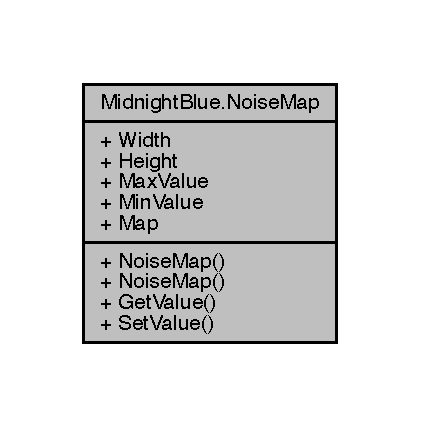
\includegraphics[width=202pt]{class_midnight_blue_1_1_noise_map__coll__graph}
\end{center}
\end{figure}
\subsection*{Public Member Functions}
\begin{DoxyCompactItemize}
\item 
\hyperlink{class_midnight_blue_1_1_noise_map_af9e93d0f595baf7f0e7c371cbbaa1809}{Noise\+Map} (Implicit\+Module\+Base fractal, int width, int height, int seed)
\begin{DoxyCompactList}\small\item\em Initializes a new instance of the T\+:\+Midnight\+Blue.\+Noise\+Map class. Initializes the fractal generator to use Simplex Noise \end{DoxyCompactList}\item 
\hyperlink{class_midnight_blue_1_1_noise_map_ad4c66d8f106a0b2c7018a5875e470e14}{Noise\+Map} (Implicit\+Module\+Base fractal, int width, int height)
\begin{DoxyCompactList}\small\item\em Initializes a new instance of the T\+:\+Midnight\+Blue.\+Noise\+Map class. Initializes the fractal generator to use Simplex Noise \end{DoxyCompactList}\item 
double \hyperlink{class_midnight_blue_1_1_noise_map_a70d9e8d99e157143eb3d1dbc3895cb9a}{Get\+Value} (int x, int y)
\begin{DoxyCompactList}\small\item\em Gets a noise value at the specified x and y coordinates. Returned as a normalized value in the range of 0 -\/ 1 \end{DoxyCompactList}\item 
void \hyperlink{class_midnight_blue_1_1_noise_map_a26d94cbea4c0377833bed064cbd36496}{Set\+Value} (int x, int y, double value)
\begin{DoxyCompactList}\small\item\em Sets a noise value at the specified x and y coordinates. Assigned as a normalized value in the range of 0 -\/ 1 \end{DoxyCompactList}\end{DoxyCompactItemize}
\subsection*{Properties}
\begin{DoxyCompactItemize}
\item 
int \hyperlink{class_midnight_blue_1_1_noise_map_a09a672256f9fb4c529e8052e428c18d2}{Width}\hspace{0.3cm}{\ttfamily  \mbox{[}get\mbox{]}}
\begin{DoxyCompactList}\small\item\em Gets the width of the noise map. \end{DoxyCompactList}\item 
int \hyperlink{class_midnight_blue_1_1_noise_map_abfffdfa7bb7a696e495bbfb2e6ac0c57}{Height}\hspace{0.3cm}{\ttfamily  \mbox{[}get\mbox{]}}
\begin{DoxyCompactList}\small\item\em Gets the height of the noise map. \end{DoxyCompactList}\item 
double \hyperlink{class_midnight_blue_1_1_noise_map_ac7a1a8a255b1512b1d09751b68636a32}{Max\+Value}\hspace{0.3cm}{\ttfamily  \mbox{[}get\mbox{]}}
\begin{DoxyCompactList}\small\item\em Gets the maximum value found in the currently generated noise map. \end{DoxyCompactList}\item 
double \hyperlink{class_midnight_blue_1_1_noise_map_a4b3978175deb42036e5a5e4f0ce5692e}{Min\+Value}\hspace{0.3cm}{\ttfamily  \mbox{[}get\mbox{]}}
\begin{DoxyCompactList}\small\item\em Gets the minimum value found in the currently generated noise map. \end{DoxyCompactList}\item 
Implicit\+Module\+Base \hyperlink{class_midnight_blue_1_1_noise_map_a428d013274d19ed0775adc6d32f00719}{Map}\hspace{0.3cm}{\ttfamily  \mbox{[}get\mbox{]}}
\begin{DoxyCompactList}\small\item\em Gets the internal map. \end{DoxyCompactList}\end{DoxyCompactItemize}


\subsection{Detailed Description}
Generates a fractal 2D map using Simplex Noise 



\subsection{Constructor \& Destructor Documentation}
\hypertarget{class_midnight_blue_1_1_noise_map_af9e93d0f595baf7f0e7c371cbbaa1809}{}\label{class_midnight_blue_1_1_noise_map_af9e93d0f595baf7f0e7c371cbbaa1809} 
\index{Midnight\+Blue\+::\+Noise\+Map@{Midnight\+Blue\+::\+Noise\+Map}!Noise\+Map@{Noise\+Map}}
\index{Noise\+Map@{Noise\+Map}!Midnight\+Blue\+::\+Noise\+Map@{Midnight\+Blue\+::\+Noise\+Map}}
\subsubsection{\texorpdfstring{Noise\+Map()}{NoiseMap()}\hspace{0.1cm}{\footnotesize\ttfamily [1/2]}}
{\footnotesize\ttfamily Midnight\+Blue.\+Noise\+Map.\+Noise\+Map (\begin{DoxyParamCaption}\item[{Implicit\+Module\+Base}]{fractal,  }\item[{int}]{width,  }\item[{int}]{height,  }\item[{int}]{seed }\end{DoxyParamCaption})\hspace{0.3cm}{\ttfamily [inline]}}



Initializes a new instance of the T\+:\+Midnight\+Blue.\+Noise\+Map class. Initializes the fractal generator to use Simplex Noise 


\begin{DoxyParams}{Parameters}
{\em width} & Width of the noise map.\\
\hline
{\em height} & Height of the noise map.\\
\hline
{\em seed} & Seed to use in generating the noise map.\\
\hline
\end{DoxyParams}
\hypertarget{class_midnight_blue_1_1_noise_map_ad4c66d8f106a0b2c7018a5875e470e14}{}\label{class_midnight_blue_1_1_noise_map_ad4c66d8f106a0b2c7018a5875e470e14} 
\index{Midnight\+Blue\+::\+Noise\+Map@{Midnight\+Blue\+::\+Noise\+Map}!Noise\+Map@{Noise\+Map}}
\index{Noise\+Map@{Noise\+Map}!Midnight\+Blue\+::\+Noise\+Map@{Midnight\+Blue\+::\+Noise\+Map}}
\subsubsection{\texorpdfstring{Noise\+Map()}{NoiseMap()}\hspace{0.1cm}{\footnotesize\ttfamily [2/2]}}
{\footnotesize\ttfamily Midnight\+Blue.\+Noise\+Map.\+Noise\+Map (\begin{DoxyParamCaption}\item[{Implicit\+Module\+Base}]{fractal,  }\item[{int}]{width,  }\item[{int}]{height }\end{DoxyParamCaption})\hspace{0.3cm}{\ttfamily [inline]}}



Initializes a new instance of the T\+:\+Midnight\+Blue.\+Noise\+Map class. Initializes the fractal generator to use Simplex Noise 


\begin{DoxyParams}{Parameters}
{\em width} & Width of the noise map.\\
\hline
{\em height} & Height of the noise map.\\
\hline
\end{DoxyParams}


\subsection{Member Function Documentation}
\hypertarget{class_midnight_blue_1_1_noise_map_a70d9e8d99e157143eb3d1dbc3895cb9a}{}\label{class_midnight_blue_1_1_noise_map_a70d9e8d99e157143eb3d1dbc3895cb9a} 
\index{Midnight\+Blue\+::\+Noise\+Map@{Midnight\+Blue\+::\+Noise\+Map}!Get\+Value@{Get\+Value}}
\index{Get\+Value@{Get\+Value}!Midnight\+Blue\+::\+Noise\+Map@{Midnight\+Blue\+::\+Noise\+Map}}
\subsubsection{\texorpdfstring{Get\+Value()}{GetValue()}}
{\footnotesize\ttfamily double Midnight\+Blue.\+Noise\+Map.\+Get\+Value (\begin{DoxyParamCaption}\item[{int}]{x,  }\item[{int}]{y }\end{DoxyParamCaption})\hspace{0.3cm}{\ttfamily [inline]}}



Gets a noise value at the specified x and y coordinates. Returned as a normalized value in the range of 0 -\/ 1 

\begin{DoxyReturn}{Returns}
The noise value.
\end{DoxyReturn}

\begin{DoxyParams}{Parameters}
{\em x} & The x coordinate.\\
\hline
{\em y} & The y coordinate.\\
\hline
\end{DoxyParams}
Here is the caller graph for this function\+:\nopagebreak
\begin{figure}[H]
\begin{center}
\leavevmode
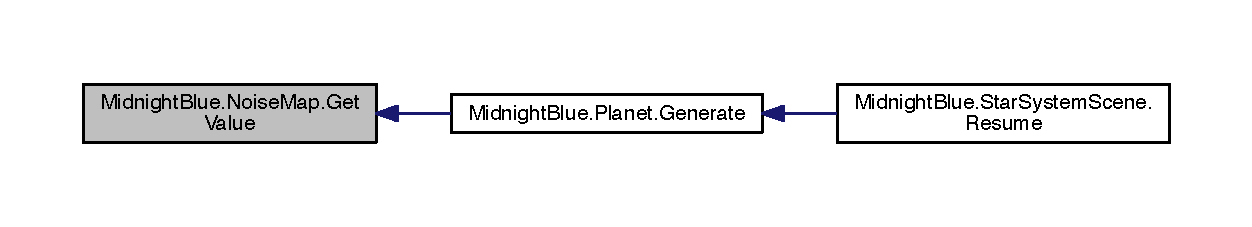
\includegraphics[width=350pt]{class_midnight_blue_1_1_noise_map_a70d9e8d99e157143eb3d1dbc3895cb9a_icgraph}
\end{center}
\end{figure}
\hypertarget{class_midnight_blue_1_1_noise_map_a26d94cbea4c0377833bed064cbd36496}{}\label{class_midnight_blue_1_1_noise_map_a26d94cbea4c0377833bed064cbd36496} 
\index{Midnight\+Blue\+::\+Noise\+Map@{Midnight\+Blue\+::\+Noise\+Map}!Set\+Value@{Set\+Value}}
\index{Set\+Value@{Set\+Value}!Midnight\+Blue\+::\+Noise\+Map@{Midnight\+Blue\+::\+Noise\+Map}}
\subsubsection{\texorpdfstring{Set\+Value()}{SetValue()}}
{\footnotesize\ttfamily void Midnight\+Blue.\+Noise\+Map.\+Set\+Value (\begin{DoxyParamCaption}\item[{int}]{x,  }\item[{int}]{y,  }\item[{double}]{value }\end{DoxyParamCaption})\hspace{0.3cm}{\ttfamily [inline]}}



Sets a noise value at the specified x and y coordinates. Assigned as a normalized value in the range of 0 -\/ 1 

\begin{DoxyReturn}{Returns}
The noise value.
\end{DoxyReturn}

\begin{DoxyParams}{Parameters}
{\em x} & The x coordinate.\\
\hline
{\em y} & The y coordinate.\\
\hline
\end{DoxyParams}
Here is the caller graph for this function\+:\nopagebreak
\begin{figure}[H]
\begin{center}
\leavevmode
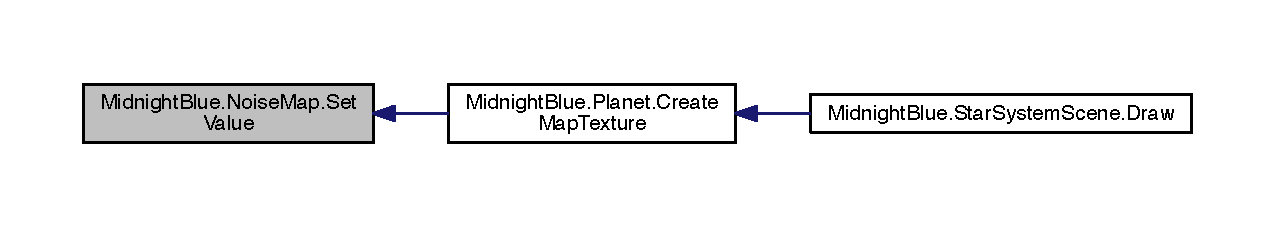
\includegraphics[width=350pt]{class_midnight_blue_1_1_noise_map_a26d94cbea4c0377833bed064cbd36496_icgraph}
\end{center}
\end{figure}


\subsection{Property Documentation}
\hypertarget{class_midnight_blue_1_1_noise_map_abfffdfa7bb7a696e495bbfb2e6ac0c57}{}\label{class_midnight_blue_1_1_noise_map_abfffdfa7bb7a696e495bbfb2e6ac0c57} 
\index{Midnight\+Blue\+::\+Noise\+Map@{Midnight\+Blue\+::\+Noise\+Map}!Height@{Height}}
\index{Height@{Height}!Midnight\+Blue\+::\+Noise\+Map@{Midnight\+Blue\+::\+Noise\+Map}}
\subsubsection{\texorpdfstring{Height}{Height}}
{\footnotesize\ttfamily int Midnight\+Blue.\+Noise\+Map.\+Height\hspace{0.3cm}{\ttfamily [get]}}



Gets the height of the noise map. 

The height.\hypertarget{class_midnight_blue_1_1_noise_map_a428d013274d19ed0775adc6d32f00719}{}\label{class_midnight_blue_1_1_noise_map_a428d013274d19ed0775adc6d32f00719} 
\index{Midnight\+Blue\+::\+Noise\+Map@{Midnight\+Blue\+::\+Noise\+Map}!Map@{Map}}
\index{Map@{Map}!Midnight\+Blue\+::\+Noise\+Map@{Midnight\+Blue\+::\+Noise\+Map}}
\subsubsection{\texorpdfstring{Map}{Map}}
{\footnotesize\ttfamily Implicit\+Module\+Base Midnight\+Blue.\+Noise\+Map.\+Map\hspace{0.3cm}{\ttfamily [get]}}



Gets the internal map. 

The map.\hypertarget{class_midnight_blue_1_1_noise_map_ac7a1a8a255b1512b1d09751b68636a32}{}\label{class_midnight_blue_1_1_noise_map_ac7a1a8a255b1512b1d09751b68636a32} 
\index{Midnight\+Blue\+::\+Noise\+Map@{Midnight\+Blue\+::\+Noise\+Map}!Max\+Value@{Max\+Value}}
\index{Max\+Value@{Max\+Value}!Midnight\+Blue\+::\+Noise\+Map@{Midnight\+Blue\+::\+Noise\+Map}}
\subsubsection{\texorpdfstring{Max\+Value}{MaxValue}}
{\footnotesize\ttfamily double Midnight\+Blue.\+Noise\+Map.\+Max\+Value\hspace{0.3cm}{\ttfamily [get]}}



Gets the maximum value found in the currently generated noise map. 

The max value.\hypertarget{class_midnight_blue_1_1_noise_map_a4b3978175deb42036e5a5e4f0ce5692e}{}\label{class_midnight_blue_1_1_noise_map_a4b3978175deb42036e5a5e4f0ce5692e} 
\index{Midnight\+Blue\+::\+Noise\+Map@{Midnight\+Blue\+::\+Noise\+Map}!Min\+Value@{Min\+Value}}
\index{Min\+Value@{Min\+Value}!Midnight\+Blue\+::\+Noise\+Map@{Midnight\+Blue\+::\+Noise\+Map}}
\subsubsection{\texorpdfstring{Min\+Value}{MinValue}}
{\footnotesize\ttfamily double Midnight\+Blue.\+Noise\+Map.\+Min\+Value\hspace{0.3cm}{\ttfamily [get]}}



Gets the minimum value found in the currently generated noise map. 

The max value.\hypertarget{class_midnight_blue_1_1_noise_map_a09a672256f9fb4c529e8052e428c18d2}{}\label{class_midnight_blue_1_1_noise_map_a09a672256f9fb4c529e8052e428c18d2} 
\index{Midnight\+Blue\+::\+Noise\+Map@{Midnight\+Blue\+::\+Noise\+Map}!Width@{Width}}
\index{Width@{Width}!Midnight\+Blue\+::\+Noise\+Map@{Midnight\+Blue\+::\+Noise\+Map}}
\subsubsection{\texorpdfstring{Width}{Width}}
{\footnotesize\ttfamily int Midnight\+Blue.\+Noise\+Map.\+Width\hspace{0.3cm}{\ttfamily [get]}}



Gets the width of the noise map. 

The width.

The documentation for this class was generated from the following file\+:\begin{DoxyCompactItemize}
\item 
Shared/src/\+Game/\+Environment/Noise\+Map.\+cs\end{DoxyCompactItemize}

\hypertarget{class_midnight_blue_1_1_planet}{}\section{Midnight\+Blue.\+Planet Class Reference}
\label{class_midnight_blue_1_1_planet}\index{Midnight\+Blue.\+Planet@{Midnight\+Blue.\+Planet}}


A fully-\/generated planet in a star system with associated texture maps.  




Collaboration diagram for Midnight\+Blue.\+Planet\+:
\nopagebreak
\begin{figure}[H]
\begin{center}
\leavevmode
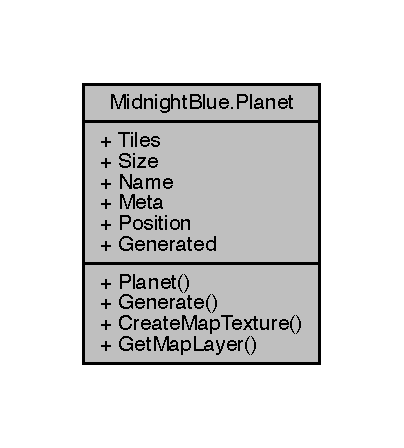
\includegraphics[width=194pt]{class_midnight_blue_1_1_planet__coll__graph}
\end{center}
\end{figure}
\subsection*{Public Member Functions}
\begin{DoxyCompactItemize}
\item 
\hyperlink{class_midnight_blue_1_1_planet_a649f87901a50e64a6423438504e468a4}{Planet} (\hyperlink{class_midnight_blue_1_1_planet_metadata}{Planet\+Metadata} meta, int seed)
\begin{DoxyCompactList}\small\item\em Initializes a new instance of the T\+:\+Midnight\+Blue.\+Planet class and sets up all noise maps ready for generation. \end{DoxyCompactList}\item 
void \hyperlink{class_midnight_blue_1_1_planet_ac7264aea3a992afb4cab0ad99c96dbb8}{Generate} (Random rand)
\begin{DoxyCompactList}\small\item\em Generates the planet after setting up with pre-\/defined metadata parameters. \end{DoxyCompactList}\item 
void \hyperlink{class_midnight_blue_1_1_planet_ae39b013905369f01902b4f28d4fc031e}{Create\+Map\+Texture} (Content\+Manager content)
\begin{DoxyCompactList}\small\item\em Creates the biome map texture and planet mask texture to use for rendering to star system view and to use as maps. \end{DoxyCompactList}\item 
Texture2D \hyperlink{class_midnight_blue_1_1_planet_ac3b3442ad8f168a8d9151386592eb270}{Get\+Map\+Layer} (string layer\+Name)
\begin{DoxyCompactList}\small\item\em Gets one of the planets generated noise map textures \end{DoxyCompactList}\end{DoxyCompactItemize}
\subsection*{Properties}
\begin{DoxyCompactItemize}
\item 
\hyperlink{class_midnight_blue_1_1_planet_tile}{Planet\+Tile} \mbox{[},\mbox{]} \hyperlink{class_midnight_blue_1_1_planet_a3e78bf28456cdfd2576b68e3ef106fc7}{Tiles}\hspace{0.3cm}{\ttfamily  \mbox{[}get\mbox{]}}
\begin{DoxyCompactList}\small\item\em Gets all the tiles in the generated planet \end{DoxyCompactList}\item 
Point \hyperlink{class_midnight_blue_1_1_planet_a10c69ed4de9c28b2e61848e3bb89c377}{Size}\hspace{0.3cm}{\ttfamily  \mbox{[}get\mbox{]}}
\begin{DoxyCompactList}\small\item\em Gets the rectangular size of the planets tile map \end{DoxyCompactList}\item 
string \hyperlink{class_midnight_blue_1_1_planet_aafbf18faf5aea56097d4f20d6b166d8a}{Name}\hspace{0.3cm}{\ttfamily  \mbox{[}get\mbox{]}}
\begin{DoxyCompactList}\small\item\em Gets the name of the planet \end{DoxyCompactList}\item 
\hyperlink{class_midnight_blue_1_1_planet_metadata}{Planet\+Metadata} \hyperlink{class_midnight_blue_1_1_planet_a064b1e2b9aa83abac4065f4a7e0c5e58}{Meta}\hspace{0.3cm}{\ttfamily  \mbox{[}get\mbox{]}}
\begin{DoxyCompactList}\small\item\em Gets the planets assigned metadata parameters \end{DoxyCompactList}\item 
Vector2 \hyperlink{class_midnight_blue_1_1_planet_a1ca1fc407e47136abb5b633e11cb8d51}{Position}\hspace{0.3cm}{\ttfamily  \mbox{[}get, set\mbox{]}}
\begin{DoxyCompactList}\small\item\em Gets or sets the planets position in the star system scene \end{DoxyCompactList}\item 
bool \hyperlink{class_midnight_blue_1_1_planet_a525e5089a0a522069f10302d9ece26e1}{Generated}\hspace{0.3cm}{\ttfamily  \mbox{[}get\mbox{]}}
\begin{DoxyCompactList}\small\item\em Gets a value indicating whether this T\+:\+Midnight\+Blue.\+Planet is generated or only setup ready to be generated. \end{DoxyCompactList}\end{DoxyCompactItemize}


\subsection{Detailed Description}
A fully-\/generated planet in a star system with associated texture maps. 



\subsection{Constructor \& Destructor Documentation}
\hypertarget{class_midnight_blue_1_1_planet_a649f87901a50e64a6423438504e468a4}{}\label{class_midnight_blue_1_1_planet_a649f87901a50e64a6423438504e468a4} 
\index{Midnight\+Blue\+::\+Planet@{Midnight\+Blue\+::\+Planet}!Planet@{Planet}}
\index{Planet@{Planet}!Midnight\+Blue\+::\+Planet@{Midnight\+Blue\+::\+Planet}}
\subsubsection{\texorpdfstring{Planet()}{Planet()}}
{\footnotesize\ttfamily Midnight\+Blue.\+Planet.\+Planet (\begin{DoxyParamCaption}\item[{\hyperlink{class_midnight_blue_1_1_planet_metadata}{Planet\+Metadata}}]{meta,  }\item[{int}]{seed }\end{DoxyParamCaption})\hspace{0.3cm}{\ttfamily [inline]}}



Initializes a new instance of the T\+:\+Midnight\+Blue.\+Planet class and sets up all noise maps ready for generation. 


\begin{DoxyParams}{Parameters}
{\em meta} & Metadata received from the planet view to act as parameters for generation.\\
\hline
{\em seed} & Seed to use in generating the map.\\
\hline
\end{DoxyParams}


\subsection{Member Function Documentation}
\hypertarget{class_midnight_blue_1_1_planet_ae39b013905369f01902b4f28d4fc031e}{}\label{class_midnight_blue_1_1_planet_ae39b013905369f01902b4f28d4fc031e} 
\index{Midnight\+Blue\+::\+Planet@{Midnight\+Blue\+::\+Planet}!Create\+Map\+Texture@{Create\+Map\+Texture}}
\index{Create\+Map\+Texture@{Create\+Map\+Texture}!Midnight\+Blue\+::\+Planet@{Midnight\+Blue\+::\+Planet}}
\subsubsection{\texorpdfstring{Create\+Map\+Texture()}{CreateMapTexture()}}
{\footnotesize\ttfamily void Midnight\+Blue.\+Planet.\+Create\+Map\+Texture (\begin{DoxyParamCaption}\item[{Content\+Manager}]{content }\end{DoxyParamCaption})\hspace{0.3cm}{\ttfamily [inline]}}



Creates the biome map texture and planet mask texture to use for rendering to star system view and to use as maps. 


\begin{DoxyParams}{Parameters}
{\em content} & Content manager for loading textures.\\
\hline
\end{DoxyParams}
Here is the call graph for this function\+:
\nopagebreak
\begin{figure}[H]
\begin{center}
\leavevmode
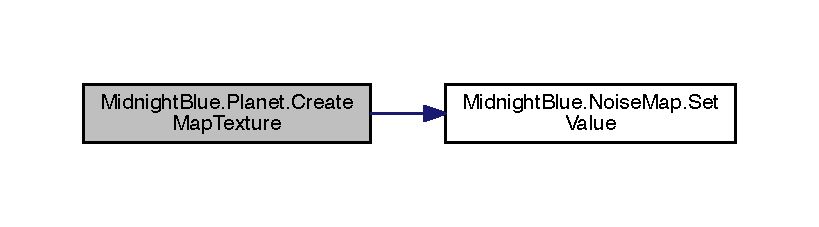
\includegraphics[width=350pt]{class_midnight_blue_1_1_planet_ae39b013905369f01902b4f28d4fc031e_cgraph}
\end{center}
\end{figure}
Here is the caller graph for this function\+:
\nopagebreak
\begin{figure}[H]
\begin{center}
\leavevmode
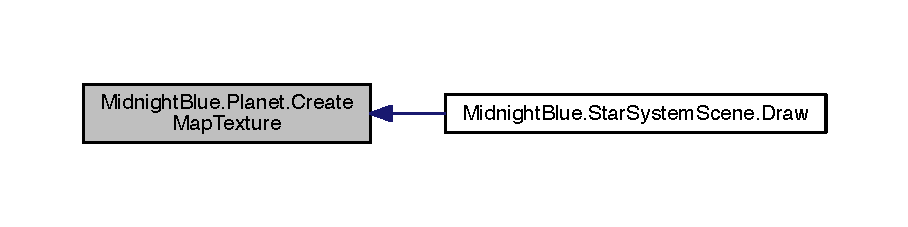
\includegraphics[width=350pt]{class_midnight_blue_1_1_planet_ae39b013905369f01902b4f28d4fc031e_icgraph}
\end{center}
\end{figure}
\hypertarget{class_midnight_blue_1_1_planet_ac7264aea3a992afb4cab0ad99c96dbb8}{}\label{class_midnight_blue_1_1_planet_ac7264aea3a992afb4cab0ad99c96dbb8} 
\index{Midnight\+Blue\+::\+Planet@{Midnight\+Blue\+::\+Planet}!Generate@{Generate}}
\index{Generate@{Generate}!Midnight\+Blue\+::\+Planet@{Midnight\+Blue\+::\+Planet}}
\subsubsection{\texorpdfstring{Generate()}{Generate()}}
{\footnotesize\ttfamily void Midnight\+Blue.\+Planet.\+Generate (\begin{DoxyParamCaption}\item[{Random}]{rand }\end{DoxyParamCaption})\hspace{0.3cm}{\ttfamily [inline]}}



Generates the planet after setting up with pre-\/defined metadata parameters. 


\begin{DoxyParams}{Parameters}
{\em rand} & Random number generator from galaxy view to use in generating the planet.\\
\hline
\end{DoxyParams}
Here is the call graph for this function\+:
\nopagebreak
\begin{figure}[H]
\begin{center}
\leavevmode
\includegraphics[width=350pt]{class_midnight_blue_1_1_planet_ac7264aea3a992afb4cab0ad99c96dbb8_cgraph}
\end{center}
\end{figure}
Here is the caller graph for this function\+:
\nopagebreak
\begin{figure}[H]
\begin{center}
\leavevmode
\includegraphics[width=350pt]{class_midnight_blue_1_1_planet_ac7264aea3a992afb4cab0ad99c96dbb8_icgraph}
\end{center}
\end{figure}
\hypertarget{class_midnight_blue_1_1_planet_ac3b3442ad8f168a8d9151386592eb270}{}\label{class_midnight_blue_1_1_planet_ac3b3442ad8f168a8d9151386592eb270} 
\index{Midnight\+Blue\+::\+Planet@{Midnight\+Blue\+::\+Planet}!Get\+Map\+Layer@{Get\+Map\+Layer}}
\index{Get\+Map\+Layer@{Get\+Map\+Layer}!Midnight\+Blue\+::\+Planet@{Midnight\+Blue\+::\+Planet}}
\subsubsection{\texorpdfstring{Get\+Map\+Layer()}{GetMapLayer()}}
{\footnotesize\ttfamily Texture2D Midnight\+Blue.\+Planet.\+Get\+Map\+Layer (\begin{DoxyParamCaption}\item[{string}]{layer\+Name }\end{DoxyParamCaption})\hspace{0.3cm}{\ttfamily [inline]}}



Gets one of the planets generated noise map textures 

\begin{DoxyReturn}{Returns}
The map layer.
\end{DoxyReturn}

\begin{DoxyParams}{Parameters}
{\em layer\+Name} & Layer name.\\
\hline
\end{DoxyParams}
Here is the caller graph for this function\+:
\nopagebreak
\begin{figure}[H]
\begin{center}
\leavevmode
\includegraphics[width=350pt]{class_midnight_blue_1_1_planet_ac3b3442ad8f168a8d9151386592eb270_icgraph}
\end{center}
\end{figure}


\subsection{Property Documentation}
\hypertarget{class_midnight_blue_1_1_planet_a525e5089a0a522069f10302d9ece26e1}{}\label{class_midnight_blue_1_1_planet_a525e5089a0a522069f10302d9ece26e1} 
\index{Midnight\+Blue\+::\+Planet@{Midnight\+Blue\+::\+Planet}!Generated@{Generated}}
\index{Generated@{Generated}!Midnight\+Blue\+::\+Planet@{Midnight\+Blue\+::\+Planet}}
\subsubsection{\texorpdfstring{Generated}{Generated}}
{\footnotesize\ttfamily bool Midnight\+Blue.\+Planet.\+Generated\hspace{0.3cm}{\ttfamily [get]}}



Gets a value indicating whether this T\+:\+Midnight\+Blue.\+Planet is generated or only setup ready to be generated. 

{\ttfamily true} if generated; otherwise, {\ttfamily false}.\hypertarget{class_midnight_blue_1_1_planet_a064b1e2b9aa83abac4065f4a7e0c5e58}{}\label{class_midnight_blue_1_1_planet_a064b1e2b9aa83abac4065f4a7e0c5e58} 
\index{Midnight\+Blue\+::\+Planet@{Midnight\+Blue\+::\+Planet}!Meta@{Meta}}
\index{Meta@{Meta}!Midnight\+Blue\+::\+Planet@{Midnight\+Blue\+::\+Planet}}
\subsubsection{\texorpdfstring{Meta}{Meta}}
{\footnotesize\ttfamily \hyperlink{class_midnight_blue_1_1_planet_metadata}{Planet\+Metadata} Midnight\+Blue.\+Planet.\+Meta\hspace{0.3cm}{\ttfamily [get]}}



Gets the planets assigned metadata parameters 

The metadata.\hypertarget{class_midnight_blue_1_1_planet_aafbf18faf5aea56097d4f20d6b166d8a}{}\label{class_midnight_blue_1_1_planet_aafbf18faf5aea56097d4f20d6b166d8a} 
\index{Midnight\+Blue\+::\+Planet@{Midnight\+Blue\+::\+Planet}!Name@{Name}}
\index{Name@{Name}!Midnight\+Blue\+::\+Planet@{Midnight\+Blue\+::\+Planet}}
\subsubsection{\texorpdfstring{Name}{Name}}
{\footnotesize\ttfamily string Midnight\+Blue.\+Planet.\+Name\hspace{0.3cm}{\ttfamily [get]}}



Gets the name of the planet 

The name.\hypertarget{class_midnight_blue_1_1_planet_a1ca1fc407e47136abb5b633e11cb8d51}{}\label{class_midnight_blue_1_1_planet_a1ca1fc407e47136abb5b633e11cb8d51} 
\index{Midnight\+Blue\+::\+Planet@{Midnight\+Blue\+::\+Planet}!Position@{Position}}
\index{Position@{Position}!Midnight\+Blue\+::\+Planet@{Midnight\+Blue\+::\+Planet}}
\subsubsection{\texorpdfstring{Position}{Position}}
{\footnotesize\ttfamily Vector2 Midnight\+Blue.\+Planet.\+Position\hspace{0.3cm}{\ttfamily [get]}, {\ttfamily [set]}}



Gets or sets the planets position in the star system scene 

The position.\hypertarget{class_midnight_blue_1_1_planet_a10c69ed4de9c28b2e61848e3bb89c377}{}\label{class_midnight_blue_1_1_planet_a10c69ed4de9c28b2e61848e3bb89c377} 
\index{Midnight\+Blue\+::\+Planet@{Midnight\+Blue\+::\+Planet}!Size@{Size}}
\index{Size@{Size}!Midnight\+Blue\+::\+Planet@{Midnight\+Blue\+::\+Planet}}
\subsubsection{\texorpdfstring{Size}{Size}}
{\footnotesize\ttfamily Point Midnight\+Blue.\+Planet.\+Size\hspace{0.3cm}{\ttfamily [get]}}



Gets the rectangular size of the planets tile map 

The size of the planet.\hypertarget{class_midnight_blue_1_1_planet_a3e78bf28456cdfd2576b68e3ef106fc7}{}\label{class_midnight_blue_1_1_planet_a3e78bf28456cdfd2576b68e3ef106fc7} 
\index{Midnight\+Blue\+::\+Planet@{Midnight\+Blue\+::\+Planet}!Tiles@{Tiles}}
\index{Tiles@{Tiles}!Midnight\+Blue\+::\+Planet@{Midnight\+Blue\+::\+Planet}}
\subsubsection{\texorpdfstring{Tiles}{Tiles}}
{\footnotesize\ttfamily \hyperlink{class_midnight_blue_1_1_planet_tile}{Planet\+Tile} \mbox{[},\mbox{]} Midnight\+Blue.\+Planet.\+Tiles\hspace{0.3cm}{\ttfamily [get]}}



Gets all the tiles in the generated planet 

The tiles.

The documentation for this class was generated from the following file\+:\begin{DoxyCompactItemize}
\item 
Shared/src/\+Game/\+Environment/Planet.\+cs\end{DoxyCompactItemize}

\hypertarget{class_midnight_blue_1_1_planet_component}{}\section{Midnight\+Blue.\+Planet\+Component Class Reference}
\label{class_midnight_blue_1_1_planet_component}\index{Midnight\+Blue.\+Planet\+Component@{Midnight\+Blue.\+Planet\+Component}}


Represents a planet entity with pre-\/generated metadata  




Inheritance diagram for Midnight\+Blue.\+Planet\+Component\+:
\nopagebreak
\begin{figure}[H]
\begin{center}
\leavevmode
\includegraphics[width=237pt]{class_midnight_blue_1_1_planet_component__inherit__graph}
\end{center}
\end{figure}


Collaboration diagram for Midnight\+Blue.\+Planet\+Component\+:
\nopagebreak
\begin{figure}[H]
\begin{center}
\leavevmode
\includegraphics[width=237pt]{class_midnight_blue_1_1_planet_component__coll__graph}
\end{center}
\end{figure}
\subsection*{Properties}
\begin{DoxyCompactItemize}
\item 
\hyperlink{class_midnight_blue_1_1_planet}{Planet} \hyperlink{class_midnight_blue_1_1_planet_component_a2beca332569c149699a62bdf33684a25}{Data}\hspace{0.3cm}{\ttfamily  \mbox{[}get, set\mbox{]}}
\begin{DoxyCompactList}\small\item\em All pre-\/generated arguments used when generating a planets map \end{DoxyCompactList}\end{DoxyCompactItemize}


\subsection{Detailed Description}
Represents a planet entity with pre-\/generated metadata 



\subsection{Property Documentation}
\hypertarget{class_midnight_blue_1_1_planet_component_a2beca332569c149699a62bdf33684a25}{}\label{class_midnight_blue_1_1_planet_component_a2beca332569c149699a62bdf33684a25} 
\index{Midnight\+Blue\+::\+Planet\+Component@{Midnight\+Blue\+::\+Planet\+Component}!Data@{Data}}
\index{Data@{Data}!Midnight\+Blue\+::\+Planet\+Component@{Midnight\+Blue\+::\+Planet\+Component}}
\subsubsection{\texorpdfstring{Data}{Data}}
{\footnotesize\ttfamily \hyperlink{class_midnight_blue_1_1_planet}{Planet} Midnight\+Blue.\+Planet\+Component.\+Data\hspace{0.3cm}{\ttfamily [get]}, {\ttfamily [set]}}



All pre-\/generated arguments used when generating a planets map 

The data.

The documentation for this class was generated from the following file\+:\begin{DoxyCompactItemize}
\item 
Shared/src/\+Game/\+Components/Planet\+Component.\+cs\end{DoxyCompactItemize}

\hypertarget{class_midnight_blue_1_1_planet_metadata}{}\section{Midnight\+Blue.\+Planet\+Metadata Class Reference}
\label{class_midnight_blue_1_1_planet_metadata}\index{Midnight\+Blue.\+Planet\+Metadata@{Midnight\+Blue.\+Planet\+Metadata}}


\hyperlink{class_midnight_blue_1_1_planet}{Planet} metadata used as information and arguments for generating the actual biome map of a planet. Required for an entity to be treated as a planet.  




Inheritance diagram for Midnight\+Blue.\+Planet\+Metadata\+:\nopagebreak
\begin{figure}[H]
\begin{center}
\leavevmode
\includegraphics[width=227pt]{class_midnight_blue_1_1_planet_metadata__inherit__graph}
\end{center}
\end{figure}


Collaboration diagram for Midnight\+Blue.\+Planet\+Metadata\+:\nopagebreak
\begin{figure}[H]
\begin{center}
\leavevmode
\includegraphics[width=227pt]{class_midnight_blue_1_1_planet_metadata__coll__graph}
\end{center}
\end{figure}
\subsection*{Properties}
\begin{DoxyCompactItemize}
\item 
string \hyperlink{class_midnight_blue_1_1_planet_metadata_a7afda7361d57bbbf9bb9d6be47167149}{Name}\hspace{0.3cm}{\ttfamily  \mbox{[}get, set\mbox{]}}
\begin{DoxyCompactList}\small\item\em Gets or sets the name of the planet. \end{DoxyCompactList}\item 
int \hyperlink{class_midnight_blue_1_1_planet_metadata_a2aa80bee630ca09d10ab12c7734e1ea4}{Radius}\hspace{0.3cm}{\ttfamily  \mbox{[}get, set\mbox{]}}
\begin{DoxyCompactList}\small\item\em Gets or sets the radius of the planet. \end{DoxyCompactList}\item 
\hyperlink{namespace_midnight_blue_a4a799009a18b57979628708589ae53e3}{Planet\+Type} \hyperlink{class_midnight_blue_1_1_planet_metadata_a9d8ec38e5924a68970df4795c6185971}{Type}\hspace{0.3cm}{\ttfamily  \mbox{[}get, set\mbox{]}}
\begin{DoxyCompactList}\small\item\em Gets or sets the type of the planet. \end{DoxyCompactList}\item 
float \hyperlink{class_midnight_blue_1_1_planet_metadata_a6902b9cd6ac9400696c6aaa74a52821f}{Surface\+Temperature}\hspace{0.3cm}{\ttfamily  \mbox{[}get, set\mbox{]}}
\begin{DoxyCompactList}\small\item\em Gets or sets the surface temperature. \end{DoxyCompactList}\item 
int \hyperlink{class_midnight_blue_1_1_planet_metadata_a6f3fe53543f04e24f107c6464b03d885}{Density}\hspace{0.3cm}{\ttfamily  \mbox{[}get, set\mbox{]}}
\begin{DoxyCompactList}\small\item\em Gets or sets the density. \end{DoxyCompactList}\item 
float \hyperlink{class_midnight_blue_1_1_planet_metadata_a918efa02de6f3aae58d4cc3804d149eb}{Habitable}\hspace{0.3cm}{\ttfamily  \mbox{[}get, set\mbox{]}}
\begin{DoxyCompactList}\small\item\em Gets or sets the score indicating the planets ability to support life. \end{DoxyCompactList}\item 
int \hyperlink{class_midnight_blue_1_1_planet_metadata_abb8cb39cd167a260d08f505ad038eb90}{Carbon}\hspace{0.3cm}{\ttfamily  \mbox{[}get, set\mbox{]}}
\begin{DoxyCompactList}\small\item\em Gets or sets the amount of carbon on the planet. \end{DoxyCompactList}\item 
int \hyperlink{class_midnight_blue_1_1_planet_metadata_a0b1319aa47d656c56cbcda678a938235}{Water}\hspace{0.3cm}{\ttfamily  \mbox{[}get, set\mbox{]}}
\begin{DoxyCompactList}\small\item\em Gets or sets the amount of water on the planet. \end{DoxyCompactList}\item 
int \hyperlink{class_midnight_blue_1_1_planet_metadata_ada2ca7bb1b67a18098a2fadd7f958ec9}{Gas}\hspace{0.3cm}{\ttfamily  \mbox{[}get, set\mbox{]}}
\begin{DoxyCompactList}\small\item\em Gets or sets the amount of gas on the planet. \end{DoxyCompactList}\item 
\hyperlink{class_midnight_blue_1_1_length}{Length} \hyperlink{class_midnight_blue_1_1_planet_metadata_a64e2d5e667ebf1d04a031ded2f68a718}{Star\+Distance}\hspace{0.3cm}{\ttfamily  \mbox{[}get, set\mbox{]}}
\begin{DoxyCompactList}\small\item\em Gets or sets the distance of this planet to its star \end{DoxyCompactList}\item 
float \hyperlink{class_midnight_blue_1_1_planet_metadata_a3fde09dbb0d471d2d50020f73089b475}{Surface\+Area}\hspace{0.3cm}{\ttfamily  \mbox{[}get\mbox{]}}
\begin{DoxyCompactList}\small\item\em Gets the surface area of the planet. Used mostly for information displays -\/ not very useful for anything else. \end{DoxyCompactList}\end{DoxyCompactItemize}


\subsection{Detailed Description}
\hyperlink{class_midnight_blue_1_1_planet}{Planet} metadata used as information and arguments for generating the actual biome map of a planet. Required for an entity to be treated as a planet. 



\subsection{Property Documentation}
\hypertarget{class_midnight_blue_1_1_planet_metadata_abb8cb39cd167a260d08f505ad038eb90}{}\label{class_midnight_blue_1_1_planet_metadata_abb8cb39cd167a260d08f505ad038eb90} 
\index{Midnight\+Blue\+::\+Planet\+Metadata@{Midnight\+Blue\+::\+Planet\+Metadata}!Carbon@{Carbon}}
\index{Carbon@{Carbon}!Midnight\+Blue\+::\+Planet\+Metadata@{Midnight\+Blue\+::\+Planet\+Metadata}}
\subsubsection{\texorpdfstring{Carbon}{Carbon}}
{\footnotesize\ttfamily int Midnight\+Blue.\+Planet\+Metadata.\+Carbon\hspace{0.3cm}{\ttfamily [get]}, {\ttfamily [set]}}



Gets or sets the amount of carbon on the planet. 

The carbon amount.\hypertarget{class_midnight_blue_1_1_planet_metadata_a6f3fe53543f04e24f107c6464b03d885}{}\label{class_midnight_blue_1_1_planet_metadata_a6f3fe53543f04e24f107c6464b03d885} 
\index{Midnight\+Blue\+::\+Planet\+Metadata@{Midnight\+Blue\+::\+Planet\+Metadata}!Density@{Density}}
\index{Density@{Density}!Midnight\+Blue\+::\+Planet\+Metadata@{Midnight\+Blue\+::\+Planet\+Metadata}}
\subsubsection{\texorpdfstring{Density}{Density}}
{\footnotesize\ttfamily int Midnight\+Blue.\+Planet\+Metadata.\+Density\hspace{0.3cm}{\ttfamily [get]}, {\ttfamily [set]}}



Gets or sets the density. 

The density.\hypertarget{class_midnight_blue_1_1_planet_metadata_ada2ca7bb1b67a18098a2fadd7f958ec9}{}\label{class_midnight_blue_1_1_planet_metadata_ada2ca7bb1b67a18098a2fadd7f958ec9} 
\index{Midnight\+Blue\+::\+Planet\+Metadata@{Midnight\+Blue\+::\+Planet\+Metadata}!Gas@{Gas}}
\index{Gas@{Gas}!Midnight\+Blue\+::\+Planet\+Metadata@{Midnight\+Blue\+::\+Planet\+Metadata}}
\subsubsection{\texorpdfstring{Gas}{Gas}}
{\footnotesize\ttfamily int Midnight\+Blue.\+Planet\+Metadata.\+Gas\hspace{0.3cm}{\ttfamily [get]}, {\ttfamily [set]}}



Gets or sets the amount of gas on the planet. 

The gas amount.\hypertarget{class_midnight_blue_1_1_planet_metadata_a918efa02de6f3aae58d4cc3804d149eb}{}\label{class_midnight_blue_1_1_planet_metadata_a918efa02de6f3aae58d4cc3804d149eb} 
\index{Midnight\+Blue\+::\+Planet\+Metadata@{Midnight\+Blue\+::\+Planet\+Metadata}!Habitable@{Habitable}}
\index{Habitable@{Habitable}!Midnight\+Blue\+::\+Planet\+Metadata@{Midnight\+Blue\+::\+Planet\+Metadata}}
\subsubsection{\texorpdfstring{Habitable}{Habitable}}
{\footnotesize\ttfamily float Midnight\+Blue.\+Planet\+Metadata.\+Habitable\hspace{0.3cm}{\ttfamily [get]}, {\ttfamily [set]}}



Gets or sets the score indicating the planets ability to support life. 

The life score.\hypertarget{class_midnight_blue_1_1_planet_metadata_a7afda7361d57bbbf9bb9d6be47167149}{}\label{class_midnight_blue_1_1_planet_metadata_a7afda7361d57bbbf9bb9d6be47167149} 
\index{Midnight\+Blue\+::\+Planet\+Metadata@{Midnight\+Blue\+::\+Planet\+Metadata}!Name@{Name}}
\index{Name@{Name}!Midnight\+Blue\+::\+Planet\+Metadata@{Midnight\+Blue\+::\+Planet\+Metadata}}
\subsubsection{\texorpdfstring{Name}{Name}}
{\footnotesize\ttfamily string Midnight\+Blue.\+Planet\+Metadata.\+Name\hspace{0.3cm}{\ttfamily [get]}, {\ttfamily [set]}}



Gets or sets the name of the planet. 

The name.\hypertarget{class_midnight_blue_1_1_planet_metadata_a2aa80bee630ca09d10ab12c7734e1ea4}{}\label{class_midnight_blue_1_1_planet_metadata_a2aa80bee630ca09d10ab12c7734e1ea4} 
\index{Midnight\+Blue\+::\+Planet\+Metadata@{Midnight\+Blue\+::\+Planet\+Metadata}!Radius@{Radius}}
\index{Radius@{Radius}!Midnight\+Blue\+::\+Planet\+Metadata@{Midnight\+Blue\+::\+Planet\+Metadata}}
\subsubsection{\texorpdfstring{Radius}{Radius}}
{\footnotesize\ttfamily int Midnight\+Blue.\+Planet\+Metadata.\+Radius\hspace{0.3cm}{\ttfamily [get]}, {\ttfamily [set]}}



Gets or sets the radius of the planet. 

The radius.\hypertarget{class_midnight_blue_1_1_planet_metadata_a64e2d5e667ebf1d04a031ded2f68a718}{}\label{class_midnight_blue_1_1_planet_metadata_a64e2d5e667ebf1d04a031ded2f68a718} 
\index{Midnight\+Blue\+::\+Planet\+Metadata@{Midnight\+Blue\+::\+Planet\+Metadata}!Star\+Distance@{Star\+Distance}}
\index{Star\+Distance@{Star\+Distance}!Midnight\+Blue\+::\+Planet\+Metadata@{Midnight\+Blue\+::\+Planet\+Metadata}}
\subsubsection{\texorpdfstring{Star\+Distance}{StarDistance}}
{\footnotesize\ttfamily \hyperlink{class_midnight_blue_1_1_length}{Length} Midnight\+Blue.\+Planet\+Metadata.\+Star\+Distance\hspace{0.3cm}{\ttfamily [get]}, {\ttfamily [set]}}



Gets or sets the distance of this planet to its star 

The star distance.\hypertarget{class_midnight_blue_1_1_planet_metadata_a3fde09dbb0d471d2d50020f73089b475}{}\label{class_midnight_blue_1_1_planet_metadata_a3fde09dbb0d471d2d50020f73089b475} 
\index{Midnight\+Blue\+::\+Planet\+Metadata@{Midnight\+Blue\+::\+Planet\+Metadata}!Surface\+Area@{Surface\+Area}}
\index{Surface\+Area@{Surface\+Area}!Midnight\+Blue\+::\+Planet\+Metadata@{Midnight\+Blue\+::\+Planet\+Metadata}}
\subsubsection{\texorpdfstring{Surface\+Area}{SurfaceArea}}
{\footnotesize\ttfamily float Midnight\+Blue.\+Planet\+Metadata.\+Surface\+Area\hspace{0.3cm}{\ttfamily [get]}}



Gets the surface area of the planet. Used mostly for information displays -\/ not very useful for anything else. 

The surface area.\hypertarget{class_midnight_blue_1_1_planet_metadata_a6902b9cd6ac9400696c6aaa74a52821f}{}\label{class_midnight_blue_1_1_planet_metadata_a6902b9cd6ac9400696c6aaa74a52821f} 
\index{Midnight\+Blue\+::\+Planet\+Metadata@{Midnight\+Blue\+::\+Planet\+Metadata}!Surface\+Temperature@{Surface\+Temperature}}
\index{Surface\+Temperature@{Surface\+Temperature}!Midnight\+Blue\+::\+Planet\+Metadata@{Midnight\+Blue\+::\+Planet\+Metadata}}
\subsubsection{\texorpdfstring{Surface\+Temperature}{SurfaceTemperature}}
{\footnotesize\ttfamily float Midnight\+Blue.\+Planet\+Metadata.\+Surface\+Temperature\hspace{0.3cm}{\ttfamily [get]}, {\ttfamily [set]}}



Gets or sets the surface temperature. 

The surface temperature.\hypertarget{class_midnight_blue_1_1_planet_metadata_a9d8ec38e5924a68970df4795c6185971}{}\label{class_midnight_blue_1_1_planet_metadata_a9d8ec38e5924a68970df4795c6185971} 
\index{Midnight\+Blue\+::\+Planet\+Metadata@{Midnight\+Blue\+::\+Planet\+Metadata}!Type@{Type}}
\index{Type@{Type}!Midnight\+Blue\+::\+Planet\+Metadata@{Midnight\+Blue\+::\+Planet\+Metadata}}
\subsubsection{\texorpdfstring{Type}{Type}}
{\footnotesize\ttfamily \hyperlink{namespace_midnight_blue_a4a799009a18b57979628708589ae53e3}{Planet\+Type} Midnight\+Blue.\+Planet\+Metadata.\+Type\hspace{0.3cm}{\ttfamily [get]}, {\ttfamily [set]}}



Gets or sets the type of the planet. 

The type.\hypertarget{class_midnight_blue_1_1_planet_metadata_a0b1319aa47d656c56cbcda678a938235}{}\label{class_midnight_blue_1_1_planet_metadata_a0b1319aa47d656c56cbcda678a938235} 
\index{Midnight\+Blue\+::\+Planet\+Metadata@{Midnight\+Blue\+::\+Planet\+Metadata}!Water@{Water}}
\index{Water@{Water}!Midnight\+Blue\+::\+Planet\+Metadata@{Midnight\+Blue\+::\+Planet\+Metadata}}
\subsubsection{\texorpdfstring{Water}{Water}}
{\footnotesize\ttfamily int Midnight\+Blue.\+Planet\+Metadata.\+Water\hspace{0.3cm}{\ttfamily [get]}, {\ttfamily [set]}}



Gets or sets the amount of water on the planet. 

The water amount.

The documentation for this class was generated from the following file\+:\begin{DoxyCompactItemize}
\item 
Shared/src/\+Game/\+Environment/Planet\+Metadata.\+cs\end{DoxyCompactItemize}

\hypertarget{class_midnight_blue_1_1_planet_scene}{}\section{Midnight\+Blue.\+Planet\+Scene Class Reference}
\label{class_midnight_blue_1_1_planet_scene}\index{Midnight\+Blue.\+Planet\+Scene@{Midnight\+Blue.\+Planet\+Scene}}


Scene active when the player is exploring a given planet.  




Inheritance diagram for Midnight\+Blue.\+Planet\+Scene\+:\nopagebreak
\begin{figure}[H]
\begin{center}
\leavevmode
\includegraphics[width=217pt]{class_midnight_blue_1_1_planet_scene__inherit__graph}
\end{center}
\end{figure}


Collaboration diagram for Midnight\+Blue.\+Planet\+Scene\+:\nopagebreak
\begin{figure}[H]
\begin{center}
\leavevmode
\includegraphics[width=217pt]{class_midnight_blue_1_1_planet_scene__coll__graph}
\end{center}
\end{figure}
\subsection*{Public Member Functions}
\begin{DoxyCompactItemize}
\item 
\hyperlink{class_midnight_blue_1_1_planet_scene_a50ee691836116a89ff549e519f895ba3}{Planet\+Scene} (\hyperlink{class_m_b2_d_1_1_entity_component_1_1_entity_map}{Entity\+Map} map, Content\+Manager content, \hyperlink{class_midnight_blue_1_1_planet}{Planet} planet)
\begin{DoxyCompactList}\small\item\em Initializes a new instance of the T\+:\+Midnight\+Blue.\+Planet\+Scene class. \end{DoxyCompactList}\item 
override void \hyperlink{class_midnight_blue_1_1_planet_scene_ac8b7e88283b22b87aa45f116b549e86f}{Initialize} ()
\begin{DoxyCompactList}\small\item\em Sets up the player and physics environment for this planet \end{DoxyCompactList}\item 
override void \hyperlink{class_midnight_blue_1_1_planet_scene_a6c84a639f27b9f7510b514969d47d1bd}{Handle\+Input} ()
\begin{DoxyCompactList}\small\item\em Handles the input for the scene. \end{DoxyCompactList}\item 
override void \hyperlink{class_midnight_blue_1_1_planet_scene_add0a85b4f754f026231aa7269259c65c}{Update} ()
\begin{DoxyCompactList}\small\item\em Updates the players position and state alongside the current biome the player is located at. \end{DoxyCompactList}\item 
override void \hyperlink{class_midnight_blue_1_1_planet_scene_af22a201631e5f8c606ec3f7463635977}{Draw} (Sprite\+Batch sprite\+Batch, Sprite\+Batch ui\+Sprite\+Batch)
\begin{DoxyCompactList}\small\item\em Draw the tilemap to the specified sprite\+Batch and ui\+Sprite\+Batch. \end{DoxyCompactList}\item 
override void \hyperlink{class_midnight_blue_1_1_planet_scene_af3aab90a13294493e1f2cd29b0fb60e6}{Exit} ()
\begin{DoxyCompactList}\small\item\em Exit this scene. \end{DoxyCompactList}\item 
override void \hyperlink{class_midnight_blue_1_1_planet_scene_abc077e1cd5f40879ca3af4224f0ff455}{Pause} ()
\begin{DoxyCompactList}\small\item\em Instantly pause the scene \end{DoxyCompactList}\item 
override void \hyperlink{class_midnight_blue_1_1_planet_scene_aa14750d3675b59462796e821b3921397}{Resume} ()
\begin{DoxyCompactList}\small\item\em Instantly resume the scene \end{DoxyCompactList}\end{DoxyCompactItemize}
\subsection*{Additional Inherited Members}


\subsection{Detailed Description}
Scene active when the player is exploring a given planet. 



\subsection{Constructor \& Destructor Documentation}
\hypertarget{class_midnight_blue_1_1_planet_scene_a50ee691836116a89ff549e519f895ba3}{}\label{class_midnight_blue_1_1_planet_scene_a50ee691836116a89ff549e519f895ba3} 
\index{Midnight\+Blue\+::\+Planet\+Scene@{Midnight\+Blue\+::\+Planet\+Scene}!Planet\+Scene@{Planet\+Scene}}
\index{Planet\+Scene@{Planet\+Scene}!Midnight\+Blue\+::\+Planet\+Scene@{Midnight\+Blue\+::\+Planet\+Scene}}
\subsubsection{\texorpdfstring{Planet\+Scene()}{PlanetScene()}}
{\footnotesize\ttfamily Midnight\+Blue.\+Planet\+Scene.\+Planet\+Scene (\begin{DoxyParamCaption}\item[{\hyperlink{class_m_b2_d_1_1_entity_component_1_1_entity_map}{Entity\+Map}}]{map,  }\item[{Content\+Manager}]{content,  }\item[{\hyperlink{class_midnight_blue_1_1_planet}{Planet}}]{planet }\end{DoxyParamCaption})\hspace{0.3cm}{\ttfamily [inline]}}



Initializes a new instance of the T\+:\+Midnight\+Blue.\+Planet\+Scene class. 


\begin{DoxyParams}{Parameters}
{\em map} & Game object map.\\
\hline
{\em content} & Content manager for loading resources.\\
\hline
{\em planet} & \hyperlink{class_midnight_blue_1_1_planet}{Planet} to use in this scene.\\
\hline
\end{DoxyParams}
Here is the call graph for this function\+:\nopagebreak
\begin{figure}[H]
\begin{center}
\leavevmode
\includegraphics[width=350pt]{class_midnight_blue_1_1_planet_scene_a50ee691836116a89ff549e519f895ba3_cgraph}
\end{center}
\end{figure}


\subsection{Member Function Documentation}
\hypertarget{class_midnight_blue_1_1_planet_scene_af22a201631e5f8c606ec3f7463635977}{}\label{class_midnight_blue_1_1_planet_scene_af22a201631e5f8c606ec3f7463635977} 
\index{Midnight\+Blue\+::\+Planet\+Scene@{Midnight\+Blue\+::\+Planet\+Scene}!Draw@{Draw}}
\index{Draw@{Draw}!Midnight\+Blue\+::\+Planet\+Scene@{Midnight\+Blue\+::\+Planet\+Scene}}
\subsubsection{\texorpdfstring{Draw()}{Draw()}}
{\footnotesize\ttfamily override void Midnight\+Blue.\+Planet\+Scene.\+Draw (\begin{DoxyParamCaption}\item[{Sprite\+Batch}]{sprite\+Batch,  }\item[{Sprite\+Batch}]{ui\+Sprite\+Batch }\end{DoxyParamCaption})\hspace{0.3cm}{\ttfamily [inline]}, {\ttfamily [virtual]}}



Draw the tilemap to the specified sprite\+Batch and ui\+Sprite\+Batch. 


\begin{DoxyParams}{Parameters}
{\em sprite\+Batch} & Sprite batch to draw world-\/based entities to.\\
\hline
{\em ui\+Sprite\+Batch} & User interface sprite batch.\\
\hline
\end{DoxyParams}


Implements \hyperlink{class_m_b2_d_1_1_scenes_1_1_scene_a932d33071ecb4c5187367825dba72324}{M\+B2\+D.\+Scenes.\+Scene}.

Here is the call graph for this function\+:\nopagebreak
\begin{figure}[H]
\begin{center}
\leavevmode
\includegraphics[width=350pt]{class_midnight_blue_1_1_planet_scene_af22a201631e5f8c606ec3f7463635977_cgraph}
\end{center}
\end{figure}
\hypertarget{class_midnight_blue_1_1_planet_scene_af3aab90a13294493e1f2cd29b0fb60e6}{}\label{class_midnight_blue_1_1_planet_scene_af3aab90a13294493e1f2cd29b0fb60e6} 
\index{Midnight\+Blue\+::\+Planet\+Scene@{Midnight\+Blue\+::\+Planet\+Scene}!Exit@{Exit}}
\index{Exit@{Exit}!Midnight\+Blue\+::\+Planet\+Scene@{Midnight\+Blue\+::\+Planet\+Scene}}
\subsubsection{\texorpdfstring{Exit()}{Exit()}}
{\footnotesize\ttfamily override void Midnight\+Blue.\+Planet\+Scene.\+Exit (\begin{DoxyParamCaption}{ }\end{DoxyParamCaption})\hspace{0.3cm}{\ttfamily [inline]}, {\ttfamily [virtual]}}



Exit this scene. 



Implements \hyperlink{class_m_b2_d_1_1_scenes_1_1_scene_a099b79e16d23b67349847999d2336813}{M\+B2\+D.\+Scenes.\+Scene}.

Here is the call graph for this function\+:\nopagebreak
\begin{figure}[H]
\begin{center}
\leavevmode
\includegraphics[width=350pt]{class_midnight_blue_1_1_planet_scene_af3aab90a13294493e1f2cd29b0fb60e6_cgraph}
\end{center}
\end{figure}
\hypertarget{class_midnight_blue_1_1_planet_scene_a6c84a639f27b9f7510b514969d47d1bd}{}\label{class_midnight_blue_1_1_planet_scene_a6c84a639f27b9f7510b514969d47d1bd} 
\index{Midnight\+Blue\+::\+Planet\+Scene@{Midnight\+Blue\+::\+Planet\+Scene}!Handle\+Input@{Handle\+Input}}
\index{Handle\+Input@{Handle\+Input}!Midnight\+Blue\+::\+Planet\+Scene@{Midnight\+Blue\+::\+Planet\+Scene}}
\subsubsection{\texorpdfstring{Handle\+Input()}{HandleInput()}}
{\footnotesize\ttfamily override void Midnight\+Blue.\+Planet\+Scene.\+Handle\+Input (\begin{DoxyParamCaption}{ }\end{DoxyParamCaption})\hspace{0.3cm}{\ttfamily [inline]}, {\ttfamily [virtual]}}



Handles the input for the scene. 



Implements \hyperlink{class_m_b2_d_1_1_scenes_1_1_scene_a476de5a885408d27ff151044d20738c8}{M\+B2\+D.\+Scenes.\+Scene}.

Here is the call graph for this function\+:\nopagebreak
\begin{figure}[H]
\begin{center}
\leavevmode
\includegraphics[width=350pt]{class_midnight_blue_1_1_planet_scene_a6c84a639f27b9f7510b514969d47d1bd_cgraph}
\end{center}
\end{figure}
\hypertarget{class_midnight_blue_1_1_planet_scene_ac8b7e88283b22b87aa45f116b549e86f}{}\label{class_midnight_blue_1_1_planet_scene_ac8b7e88283b22b87aa45f116b549e86f} 
\index{Midnight\+Blue\+::\+Planet\+Scene@{Midnight\+Blue\+::\+Planet\+Scene}!Initialize@{Initialize}}
\index{Initialize@{Initialize}!Midnight\+Blue\+::\+Planet\+Scene@{Midnight\+Blue\+::\+Planet\+Scene}}
\subsubsection{\texorpdfstring{Initialize()}{Initialize()}}
{\footnotesize\ttfamily override void Midnight\+Blue.\+Planet\+Scene.\+Initialize (\begin{DoxyParamCaption}{ }\end{DoxyParamCaption})\hspace{0.3cm}{\ttfamily [inline]}, {\ttfamily [virtual]}}



Sets up the player and physics environment for this planet 



Implements \hyperlink{class_m_b2_d_1_1_scenes_1_1_scene_a081b4f8866936b495bdce388a7c96c25}{M\+B2\+D.\+Scenes.\+Scene}.

\hypertarget{class_midnight_blue_1_1_planet_scene_abc077e1cd5f40879ca3af4224f0ff455}{}\label{class_midnight_blue_1_1_planet_scene_abc077e1cd5f40879ca3af4224f0ff455} 
\index{Midnight\+Blue\+::\+Planet\+Scene@{Midnight\+Blue\+::\+Planet\+Scene}!Pause@{Pause}}
\index{Pause@{Pause}!Midnight\+Blue\+::\+Planet\+Scene@{Midnight\+Blue\+::\+Planet\+Scene}}
\subsubsection{\texorpdfstring{Pause()}{Pause()}}
{\footnotesize\ttfamily override void Midnight\+Blue.\+Planet\+Scene.\+Pause (\begin{DoxyParamCaption}{ }\end{DoxyParamCaption})\hspace{0.3cm}{\ttfamily [inline]}, {\ttfamily [virtual]}}



Instantly pause the scene 



Implements \hyperlink{class_m_b2_d_1_1_scenes_1_1_scene_a0661eff0223150fa8e9ea88145409e5d}{M\+B2\+D.\+Scenes.\+Scene}.

\hypertarget{class_midnight_blue_1_1_planet_scene_aa14750d3675b59462796e821b3921397}{}\label{class_midnight_blue_1_1_planet_scene_aa14750d3675b59462796e821b3921397} 
\index{Midnight\+Blue\+::\+Planet\+Scene@{Midnight\+Blue\+::\+Planet\+Scene}!Resume@{Resume}}
\index{Resume@{Resume}!Midnight\+Blue\+::\+Planet\+Scene@{Midnight\+Blue\+::\+Planet\+Scene}}
\subsubsection{\texorpdfstring{Resume()}{Resume()}}
{\footnotesize\ttfamily override void Midnight\+Blue.\+Planet\+Scene.\+Resume (\begin{DoxyParamCaption}{ }\end{DoxyParamCaption})\hspace{0.3cm}{\ttfamily [inline]}, {\ttfamily [virtual]}}



Instantly resume the scene 



Implements \hyperlink{class_m_b2_d_1_1_scenes_1_1_scene_ad13639db22b059a1b714eefd9d927735}{M\+B2\+D.\+Scenes.\+Scene}.

\hypertarget{class_midnight_blue_1_1_planet_scene_add0a85b4f754f026231aa7269259c65c}{}\label{class_midnight_blue_1_1_planet_scene_add0a85b4f754f026231aa7269259c65c} 
\index{Midnight\+Blue\+::\+Planet\+Scene@{Midnight\+Blue\+::\+Planet\+Scene}!Update@{Update}}
\index{Update@{Update}!Midnight\+Blue\+::\+Planet\+Scene@{Midnight\+Blue\+::\+Planet\+Scene}}
\subsubsection{\texorpdfstring{Update()}{Update()}}
{\footnotesize\ttfamily override void Midnight\+Blue.\+Planet\+Scene.\+Update (\begin{DoxyParamCaption}{ }\end{DoxyParamCaption})\hspace{0.3cm}{\ttfamily [inline]}, {\ttfamily [virtual]}}



Updates the players position and state alongside the current biome the player is located at. 



Implements \hyperlink{class_m_b2_d_1_1_scenes_1_1_scene_a779de7c1ab23b698dcde3a228324a991}{M\+B2\+D.\+Scenes.\+Scene}.

Here is the call graph for this function\+:\nopagebreak
\begin{figure}[H]
\begin{center}
\leavevmode
\includegraphics[width=350pt]{class_midnight_blue_1_1_planet_scene_add0a85b4f754f026231aa7269259c65c_cgraph}
\end{center}
\end{figure}


The documentation for this class was generated from the following file\+:\begin{DoxyCompactItemize}
\item 
Shared/src/\+Game/\+Scenes/Planet\+Scene.\+cs\end{DoxyCompactItemize}

\hypertarget{class_midnight_blue_1_1_planet_tile}{}\section{Midnight\+Blue.\+Planet\+Tile Class Reference}
\label{class_midnight_blue_1_1_planet_tile}\index{Midnight\+Blue.\+Planet\+Tile@{Midnight\+Blue.\+Planet\+Tile}}


A tile type used in planet tilemaps  




Inheritance diagram for Midnight\+Blue.\+Planet\+Tile\+:\nopagebreak
\begin{figure}[H]
\begin{center}
\leavevmode
\includegraphics[width=201pt]{class_midnight_blue_1_1_planet_tile__inherit__graph}
\end{center}
\end{figure}


Collaboration diagram for Midnight\+Blue.\+Planet\+Tile\+:\nopagebreak
\begin{figure}[H]
\begin{center}
\leavevmode
\includegraphics[width=201pt]{class_midnight_blue_1_1_planet_tile__coll__graph}
\end{center}
\end{figure}
\subsection*{Public Member Functions}
\begin{DoxyCompactItemize}
\item 
\hyperlink{class_midnight_blue_1_1_planet_tile_aa8fd125394504682bd0c2f2d9d28622b}{Planet\+Tile} (double height, double moisture, double temperature, Random rand)
\begin{DoxyCompactList}\small\item\em Initializes a new instance of the T\+:\+Midnight\+Blue.\+Planet\+Tile class, generates a biome and specifies collision data based on its biome type. \end{DoxyCompactList}\item 
int \hyperlink{class_midnight_blue_1_1_planet_tile_a0ba5d9886790e8f8d9e54e1873d5565b}{Get\+Texture\+ID} (\hyperlink{namespace_midnight_blue_a8a6ba5637b64c3eb991f00d48decf381}{Biome} biome, Random rand)
\begin{DoxyCompactList}\small\item\em Gets the ID of a biomes texture region for use in a tilemap \end{DoxyCompactList}\item 
Color \hyperlink{class_midnight_blue_1_1_planet_tile_a0efc70f73aaf5a252cfe6b96deb9aa22}{Get\+Color} (\hyperlink{namespace_midnight_blue_a8a6ba5637b64c3eb991f00d48decf381}{Biome} biome)
\begin{DoxyCompactList}\small\item\em Gets the color of a tile in the minimap based on its biome. \end{DoxyCompactList}\end{DoxyCompactItemize}
\subsection*{Properties}
\begin{DoxyCompactItemize}
\item 
\hyperlink{namespace_midnight_blue_a86f8aaa0bbb651a6a094d3eb95f799e0}{Height\+Level} \hyperlink{class_midnight_blue_1_1_planet_tile_a64d018817a484ab3b4559773b0971974}{Height}\hspace{0.3cm}{\ttfamily  \mbox{[}get\mbox{]}}
\begin{DoxyCompactList}\small\item\em Gets the height category of the tile. \end{DoxyCompactList}\item 
\hyperlink{namespace_midnight_blue_a7428767e7fc0b52bab6cb270f8354e1d}{Moisture\+Level} \hyperlink{class_midnight_blue_1_1_planet_tile_a867d91b1185e400c608eea5e20ba4614}{Moisture}\hspace{0.3cm}{\ttfamily  \mbox{[}get\mbox{]}}
\begin{DoxyCompactList}\small\item\em Gets the moisture category of the tile. \end{DoxyCompactList}\item 
\hyperlink{namespace_midnight_blue_a6ea6484178cbe707f25d1a0ed56db7ab}{Temperature\+Level} \hyperlink{class_midnight_blue_1_1_planet_tile_a7e2a7e01274b4ea505871b115b8534ae}{Temperature}\hspace{0.3cm}{\ttfamily  \mbox{[}get\mbox{]}}
\begin{DoxyCompactList}\small\item\em Gets the temperature category of the tile. \end{DoxyCompactList}\item 
\hyperlink{namespace_midnight_blue_a8a6ba5637b64c3eb991f00d48decf381}{Biome} \hyperlink{class_midnight_blue_1_1_planet_tile_a56f9f50efa0b740b3ce229cb4170fd97}{Biome}\hspace{0.3cm}{\ttfamily  \mbox{[}get\mbox{]}}
\begin{DoxyCompactList}\small\item\em Gets the biome category of the tile. \end{DoxyCompactList}\end{DoxyCompactItemize}


\subsection{Detailed Description}
A tile type used in planet tilemaps 



\subsection{Constructor \& Destructor Documentation}
\hypertarget{class_midnight_blue_1_1_planet_tile_aa8fd125394504682bd0c2f2d9d28622b}{}\label{class_midnight_blue_1_1_planet_tile_aa8fd125394504682bd0c2f2d9d28622b} 
\index{Midnight\+Blue\+::\+Planet\+Tile@{Midnight\+Blue\+::\+Planet\+Tile}!Planet\+Tile@{Planet\+Tile}}
\index{Planet\+Tile@{Planet\+Tile}!Midnight\+Blue\+::\+Planet\+Tile@{Midnight\+Blue\+::\+Planet\+Tile}}
\subsubsection{\texorpdfstring{Planet\+Tile()}{PlanetTile()}}
{\footnotesize\ttfamily Midnight\+Blue.\+Planet\+Tile.\+Planet\+Tile (\begin{DoxyParamCaption}\item[{double}]{height,  }\item[{double}]{moisture,  }\item[{double}]{temperature,  }\item[{Random}]{rand }\end{DoxyParamCaption})\hspace{0.3cm}{\ttfamily [inline]}}



Initializes a new instance of the T\+:\+Midnight\+Blue.\+Planet\+Tile class, generates a biome and specifies collision data based on its biome type. 


\begin{DoxyParams}{Parameters}
{\em height} & Height value to use in generation.\\
\hline
{\em moisture} & Moisture value to use in generation.\\
\hline
{\em temperature} & Temperature value to use in generation.\\
\hline
{\em rand} & Random number generator used in biome generation.\\
\hline
\end{DoxyParams}
Here is the call graph for this function\+:\nopagebreak
\begin{figure}[H]
\begin{center}
\leavevmode
\includegraphics[width=350pt]{class_midnight_blue_1_1_planet_tile_aa8fd125394504682bd0c2f2d9d28622b_cgraph}
\end{center}
\end{figure}


\subsection{Member Function Documentation}
\hypertarget{class_midnight_blue_1_1_planet_tile_a0efc70f73aaf5a252cfe6b96deb9aa22}{}\label{class_midnight_blue_1_1_planet_tile_a0efc70f73aaf5a252cfe6b96deb9aa22} 
\index{Midnight\+Blue\+::\+Planet\+Tile@{Midnight\+Blue\+::\+Planet\+Tile}!Get\+Color@{Get\+Color}}
\index{Get\+Color@{Get\+Color}!Midnight\+Blue\+::\+Planet\+Tile@{Midnight\+Blue\+::\+Planet\+Tile}}
\subsubsection{\texorpdfstring{Get\+Color()}{GetColor()}}
{\footnotesize\ttfamily Color Midnight\+Blue.\+Planet\+Tile.\+Get\+Color (\begin{DoxyParamCaption}\item[{\hyperlink{namespace_midnight_blue_a8a6ba5637b64c3eb991f00d48decf381}{Biome}}]{biome }\end{DoxyParamCaption})\hspace{0.3cm}{\ttfamily [inline]}}



Gets the color of a tile in the minimap based on its biome. 

\begin{DoxyReturn}{Returns}
The color.
\end{DoxyReturn}

\begin{DoxyParams}{Parameters}
{\em biome} & Biome to get.\\
\hline
\end{DoxyParams}
Here is the caller graph for this function\+:\nopagebreak
\begin{figure}[H]
\begin{center}
\leavevmode
\includegraphics[width=350pt]{class_midnight_blue_1_1_planet_tile_a0efc70f73aaf5a252cfe6b96deb9aa22_icgraph}
\end{center}
\end{figure}
\hypertarget{class_midnight_blue_1_1_planet_tile_a0ba5d9886790e8f8d9e54e1873d5565b}{}\label{class_midnight_blue_1_1_planet_tile_a0ba5d9886790e8f8d9e54e1873d5565b} 
\index{Midnight\+Blue\+::\+Planet\+Tile@{Midnight\+Blue\+::\+Planet\+Tile}!Get\+Texture\+ID@{Get\+Texture\+ID}}
\index{Get\+Texture\+ID@{Get\+Texture\+ID}!Midnight\+Blue\+::\+Planet\+Tile@{Midnight\+Blue\+::\+Planet\+Tile}}
\subsubsection{\texorpdfstring{Get\+Texture\+I\+D()}{GetTextureID()}}
{\footnotesize\ttfamily int Midnight\+Blue.\+Planet\+Tile.\+Get\+Texture\+ID (\begin{DoxyParamCaption}\item[{\hyperlink{namespace_midnight_blue_a8a6ba5637b64c3eb991f00d48decf381}{Biome}}]{biome,  }\item[{Random}]{rand }\end{DoxyParamCaption})\hspace{0.3cm}{\ttfamily [inline]}}



Gets the ID of a biomes texture region for use in a tilemap 

\begin{DoxyReturn}{Returns}
The texture region identifier.
\end{DoxyReturn}

\begin{DoxyParams}{Parameters}
{\em biome} & Biome to get.\\
\hline
{\em rand} & Random number generator to use for varied region id\textquotesingle{}s.\\
\hline
\end{DoxyParams}
Here is the caller graph for this function\+:\nopagebreak
\begin{figure}[H]
\begin{center}
\leavevmode
\includegraphics[width=350pt]{class_midnight_blue_1_1_planet_tile_a0ba5d9886790e8f8d9e54e1873d5565b_icgraph}
\end{center}
\end{figure}


\subsection{Property Documentation}
\hypertarget{class_midnight_blue_1_1_planet_tile_a56f9f50efa0b740b3ce229cb4170fd97}{}\label{class_midnight_blue_1_1_planet_tile_a56f9f50efa0b740b3ce229cb4170fd97} 
\index{Midnight\+Blue\+::\+Planet\+Tile@{Midnight\+Blue\+::\+Planet\+Tile}!Biome@{Biome}}
\index{Biome@{Biome}!Midnight\+Blue\+::\+Planet\+Tile@{Midnight\+Blue\+::\+Planet\+Tile}}
\subsubsection{\texorpdfstring{Biome}{Biome}}
{\footnotesize\ttfamily \hyperlink{namespace_midnight_blue_a8a6ba5637b64c3eb991f00d48decf381}{Biome} Midnight\+Blue.\+Planet\+Tile.\+Biome\hspace{0.3cm}{\ttfamily [get]}}



Gets the biome category of the tile. 

The biome category.\hypertarget{class_midnight_blue_1_1_planet_tile_a64d018817a484ab3b4559773b0971974}{}\label{class_midnight_blue_1_1_planet_tile_a64d018817a484ab3b4559773b0971974} 
\index{Midnight\+Blue\+::\+Planet\+Tile@{Midnight\+Blue\+::\+Planet\+Tile}!Height@{Height}}
\index{Height@{Height}!Midnight\+Blue\+::\+Planet\+Tile@{Midnight\+Blue\+::\+Planet\+Tile}}
\subsubsection{\texorpdfstring{Height}{Height}}
{\footnotesize\ttfamily \hyperlink{namespace_midnight_blue_a86f8aaa0bbb651a6a094d3eb95f799e0}{Height\+Level} Midnight\+Blue.\+Planet\+Tile.\+Height\hspace{0.3cm}{\ttfamily [get]}}



Gets the height category of the tile. 

The height category.\hypertarget{class_midnight_blue_1_1_planet_tile_a867d91b1185e400c608eea5e20ba4614}{}\label{class_midnight_blue_1_1_planet_tile_a867d91b1185e400c608eea5e20ba4614} 
\index{Midnight\+Blue\+::\+Planet\+Tile@{Midnight\+Blue\+::\+Planet\+Tile}!Moisture@{Moisture}}
\index{Moisture@{Moisture}!Midnight\+Blue\+::\+Planet\+Tile@{Midnight\+Blue\+::\+Planet\+Tile}}
\subsubsection{\texorpdfstring{Moisture}{Moisture}}
{\footnotesize\ttfamily \hyperlink{namespace_midnight_blue_a7428767e7fc0b52bab6cb270f8354e1d}{Moisture\+Level} Midnight\+Blue.\+Planet\+Tile.\+Moisture\hspace{0.3cm}{\ttfamily [get]}}



Gets the moisture category of the tile. 

The moisture category.\hypertarget{class_midnight_blue_1_1_planet_tile_a7e2a7e01274b4ea505871b115b8534ae}{}\label{class_midnight_blue_1_1_planet_tile_a7e2a7e01274b4ea505871b115b8534ae} 
\index{Midnight\+Blue\+::\+Planet\+Tile@{Midnight\+Blue\+::\+Planet\+Tile}!Temperature@{Temperature}}
\index{Temperature@{Temperature}!Midnight\+Blue\+::\+Planet\+Tile@{Midnight\+Blue\+::\+Planet\+Tile}}
\subsubsection{\texorpdfstring{Temperature}{Temperature}}
{\footnotesize\ttfamily \hyperlink{namespace_midnight_blue_a6ea6484178cbe707f25d1a0ed56db7ab}{Temperature\+Level} Midnight\+Blue.\+Planet\+Tile.\+Temperature\hspace{0.3cm}{\ttfamily [get]}}



Gets the temperature category of the tile. 

The temperature category.

The documentation for this class was generated from the following file\+:\begin{DoxyCompactItemize}
\item 
Shared/src/\+Game/\+Environment/Planet\+Tile.\+cs\end{DoxyCompactItemize}

\hypertarget{class_midnight_blue_1_1_ship_controller}{}\section{Midnight\+Blue.\+Ship\+Controller Class Reference}
\label{class_midnight_blue_1_1_ship_controller}\index{Midnight\+Blue.\+Ship\+Controller@{Midnight\+Blue.\+Ship\+Controller}}


Controls a ships movement and actions  




Inheritance diagram for Midnight\+Blue.\+Ship\+Controller\+:
\nopagebreak
\begin{figure}[H]
\begin{center}
\leavevmode
\includegraphics[width=220pt]{class_midnight_blue_1_1_ship_controller__inherit__graph}
\end{center}
\end{figure}


Collaboration diagram for Midnight\+Blue.\+Ship\+Controller\+:
\nopagebreak
\begin{figure}[H]
\begin{center}
\leavevmode
\includegraphics[width=220pt]{class_midnight_blue_1_1_ship_controller__coll__graph}
\end{center}
\end{figure}
\subsection*{Public Member Functions}
\begin{DoxyCompactItemize}
\item 
\hyperlink{class_midnight_blue_1_1_ship_controller_a07d38d2b98b9b132f1eff9cc8879f278}{Ship\+Controller} ()
\begin{DoxyCompactList}\small\item\em Initializes a new instance of the T\+:\+Midnight\+Blue.\+Ship\+Controller class and assigns all default input and key mappings. \end{DoxyCompactList}\end{DoxyCompactItemize}
\subsection*{Properties}
\begin{DoxyCompactItemize}
\item 
\hyperlink{class_midnight_blue_1_1_engine_1_1_i_o_1_1_input_map}{Input\+Map} \hyperlink{class_midnight_blue_1_1_ship_controller_a50136c59b5a0e80d280aec4b6de46414}{Input\+Map}\hspace{0.3cm}{\ttfamily  \mbox{[}get\mbox{]}}
\begin{DoxyCompactList}\small\item\em Gets the input map. \end{DoxyCompactList}\item 
\hyperlink{namespace_midnight_blue_a46fd3250d826e0dec67892328d5b368c}{Ship\+State} \hyperlink{class_midnight_blue_1_1_ship_controller_a032da447be3b66b7998349ae825d4edb}{State}\hspace{0.3cm}{\ttfamily  \mbox{[}get, set\mbox{]}}
\begin{DoxyCompactList}\small\item\em Gets or sets the current travel state of the ship. \end{DoxyCompactList}\item 
bool \hyperlink{class_midnight_blue_1_1_ship_controller_ad07cfa737db5a712aedcc2528b953683}{Is\+Landable}\hspace{0.3cm}{\ttfamily  \mbox{[}get, set\mbox{]}}
\begin{DoxyCompactList}\small\item\em Gets or sets a value indicating whether this T\+:\+Midnight\+Blue.\+Ship\+Controller is able to be landed when the entity calls their \hyperlink{class_midnight_blue_1_1_land_command}{Land\+Command}. \end{DoxyCompactList}\end{DoxyCompactItemize}


\subsection{Detailed Description}
Controls a ships movement and actions 



\subsection{Constructor \& Destructor Documentation}
\hypertarget{class_midnight_blue_1_1_ship_controller_a07d38d2b98b9b132f1eff9cc8879f278}{}\label{class_midnight_blue_1_1_ship_controller_a07d38d2b98b9b132f1eff9cc8879f278} 
\index{Midnight\+Blue\+::\+Ship\+Controller@{Midnight\+Blue\+::\+Ship\+Controller}!Ship\+Controller@{Ship\+Controller}}
\index{Ship\+Controller@{Ship\+Controller}!Midnight\+Blue\+::\+Ship\+Controller@{Midnight\+Blue\+::\+Ship\+Controller}}
\subsubsection{\texorpdfstring{Ship\+Controller()}{ShipController()}}
{\footnotesize\ttfamily Midnight\+Blue.\+Ship\+Controller.\+Ship\+Controller (\begin{DoxyParamCaption}{ }\end{DoxyParamCaption})\hspace{0.3cm}{\ttfamily [inline]}}



Initializes a new instance of the T\+:\+Midnight\+Blue.\+Ship\+Controller class and assigns all default input and key mappings. 



\subsection{Property Documentation}
\hypertarget{class_midnight_blue_1_1_ship_controller_a50136c59b5a0e80d280aec4b6de46414}{}\label{class_midnight_blue_1_1_ship_controller_a50136c59b5a0e80d280aec4b6de46414} 
\index{Midnight\+Blue\+::\+Ship\+Controller@{Midnight\+Blue\+::\+Ship\+Controller}!Input\+Map@{Input\+Map}}
\index{Input\+Map@{Input\+Map}!Midnight\+Blue\+::\+Ship\+Controller@{Midnight\+Blue\+::\+Ship\+Controller}}
\subsubsection{\texorpdfstring{Input\+Map}{InputMap}}
{\footnotesize\ttfamily \hyperlink{class_midnight_blue_1_1_engine_1_1_i_o_1_1_input_map}{Input\+Map} Midnight\+Blue.\+Ship\+Controller.\+Input\+Map\hspace{0.3cm}{\ttfamily [get]}}



Gets the input map. 

The input map.\hypertarget{class_midnight_blue_1_1_ship_controller_ad07cfa737db5a712aedcc2528b953683}{}\label{class_midnight_blue_1_1_ship_controller_ad07cfa737db5a712aedcc2528b953683} 
\index{Midnight\+Blue\+::\+Ship\+Controller@{Midnight\+Blue\+::\+Ship\+Controller}!Is\+Landable@{Is\+Landable}}
\index{Is\+Landable@{Is\+Landable}!Midnight\+Blue\+::\+Ship\+Controller@{Midnight\+Blue\+::\+Ship\+Controller}}
\subsubsection{\texorpdfstring{Is\+Landable}{IsLandable}}
{\footnotesize\ttfamily bool Midnight\+Blue.\+Ship\+Controller.\+Is\+Landable\hspace{0.3cm}{\ttfamily [get]}, {\ttfamily [set]}}



Gets or sets a value indicating whether this T\+:\+Midnight\+Blue.\+Ship\+Controller is able to be landed when the entity calls their \hyperlink{class_midnight_blue_1_1_land_command}{Land\+Command}. 

{\ttfamily true} if is landable; otherwise, {\ttfamily false}.\hypertarget{class_midnight_blue_1_1_ship_controller_a032da447be3b66b7998349ae825d4edb}{}\label{class_midnight_blue_1_1_ship_controller_a032da447be3b66b7998349ae825d4edb} 
\index{Midnight\+Blue\+::\+Ship\+Controller@{Midnight\+Blue\+::\+Ship\+Controller}!State@{State}}
\index{State@{State}!Midnight\+Blue\+::\+Ship\+Controller@{Midnight\+Blue\+::\+Ship\+Controller}}
\subsubsection{\texorpdfstring{State}{State}}
{\footnotesize\ttfamily \hyperlink{namespace_midnight_blue_a46fd3250d826e0dec67892328d5b368c}{Ship\+State} Midnight\+Blue.\+Ship\+Controller.\+State\hspace{0.3cm}{\ttfamily [get]}, {\ttfamily [set]}}



Gets or sets the current travel state of the ship. 

The ships travelling state.

The documentation for this class was generated from the following file\+:\begin{DoxyCompactItemize}
\item 
Shared/src/\+Game/\+Components/Ship\+Controller.\+cs\end{DoxyCompactItemize}

\hypertarget{class_midnight_blue_1_1_ship_input_system}{}\section{Midnight\+Blue.\+Ship\+Input\+System Class Reference}
\label{class_midnight_blue_1_1_ship_input_system}\index{Midnight\+Blue.\+Ship\+Input\+System@{Midnight\+Blue.\+Ship\+Input\+System}}


Handles moving the ship forward and backwards.  




Inheritance diagram for Midnight\+Blue.\+Ship\+Input\+System\+:
\nopagebreak
\begin{figure}[H]
\begin{center}
\leavevmode
\includegraphics[width=232pt]{class_midnight_blue_1_1_ship_input_system__inherit__graph}
\end{center}
\end{figure}


Collaboration diagram for Midnight\+Blue.\+Ship\+Input\+System\+:
\nopagebreak
\begin{figure}[H]
\begin{center}
\leavevmode
\includegraphics[width=232pt]{class_midnight_blue_1_1_ship_input_system__coll__graph}
\end{center}
\end{figure}
\subsection*{Public Member Functions}
\begin{DoxyCompactItemize}
\item 
\hyperlink{class_midnight_blue_1_1_ship_input_system_ad7f804f91939a651c8e53ddb6bf55db6}{Ship\+Input\+System} ()
\begin{DoxyCompactList}\small\item\em Initializes a new instance of the T\+:\+Midnight\+Blue.\+Ship\+Input\+System class. \end{DoxyCompactList}\end{DoxyCompactItemize}
\subsection*{Protected Member Functions}
\begin{DoxyCompactItemize}
\item 
override void \hyperlink{class_midnight_blue_1_1_ship_input_system_ac504beb5b6afa47ca4618d9683e46946}{Process} (Entity entity)
\begin{DoxyCompactList}\small\item\em Uses the entities ship controller to move forward and backward \end{DoxyCompactList}\end{DoxyCompactItemize}


\subsection{Detailed Description}
Handles moving the ship forward and backwards. 



\subsection{Constructor \& Destructor Documentation}
\hypertarget{class_midnight_blue_1_1_ship_input_system_ad7f804f91939a651c8e53ddb6bf55db6}{}\label{class_midnight_blue_1_1_ship_input_system_ad7f804f91939a651c8e53ddb6bf55db6} 
\index{Midnight\+Blue\+::\+Ship\+Input\+System@{Midnight\+Blue\+::\+Ship\+Input\+System}!Ship\+Input\+System@{Ship\+Input\+System}}
\index{Ship\+Input\+System@{Ship\+Input\+System}!Midnight\+Blue\+::\+Ship\+Input\+System@{Midnight\+Blue\+::\+Ship\+Input\+System}}
\subsubsection{\texorpdfstring{Ship\+Input\+System()}{ShipInputSystem()}}
{\footnotesize\ttfamily Midnight\+Blue.\+Ship\+Input\+System.\+Ship\+Input\+System (\begin{DoxyParamCaption}{ }\end{DoxyParamCaption})\hspace{0.3cm}{\ttfamily [inline]}}



Initializes a new instance of the T\+:\+Midnight\+Blue.\+Ship\+Input\+System class. 



\subsection{Member Function Documentation}
\hypertarget{class_midnight_blue_1_1_ship_input_system_ac504beb5b6afa47ca4618d9683e46946}{}\label{class_midnight_blue_1_1_ship_input_system_ac504beb5b6afa47ca4618d9683e46946} 
\index{Midnight\+Blue\+::\+Ship\+Input\+System@{Midnight\+Blue\+::\+Ship\+Input\+System}!Process@{Process}}
\index{Process@{Process}!Midnight\+Blue\+::\+Ship\+Input\+System@{Midnight\+Blue\+::\+Ship\+Input\+System}}
\subsubsection{\texorpdfstring{Process()}{Process()}}
{\footnotesize\ttfamily override void Midnight\+Blue.\+Ship\+Input\+System.\+Process (\begin{DoxyParamCaption}\item[{Entity}]{entity }\end{DoxyParamCaption})\hspace{0.3cm}{\ttfamily [inline]}, {\ttfamily [protected]}}



Uses the entities ship controller to move forward and backward 


\begin{DoxyParams}{Parameters}
{\em entity} & Entity to process.\\
\hline
\end{DoxyParams}


The documentation for this class was generated from the following file\+:\begin{DoxyCompactItemize}
\item 
Shared/src/\+Game/\+Systems/Ship\+Input\+System.\+cs\end{DoxyCompactItemize}

\hypertarget{class_midnight_blue_1_1_star_system}{}\section{Midnight\+Blue.\+Star\+System Class Reference}
\label{class_midnight_blue_1_1_star_system}\index{Midnight\+Blue.\+Star\+System@{Midnight\+Blue.\+Star\+System}}


Represents an star system entity to be used in the galaxy view  




Inheritance diagram for Midnight\+Blue.\+Star\+System\+:\nopagebreak
\begin{figure}[H]
\begin{center}
\leavevmode
\includegraphics[width=208pt]{class_midnight_blue_1_1_star_system__inherit__graph}
\end{center}
\end{figure}


Collaboration diagram for Midnight\+Blue.\+Star\+System\+:\nopagebreak
\begin{figure}[H]
\begin{center}
\leavevmode
\includegraphics[width=208pt]{class_midnight_blue_1_1_star_system__coll__graph}
\end{center}
\end{figure}
\subsection*{Public Member Functions}
\begin{DoxyCompactItemize}
\item 
\hyperlink{class_midnight_blue_1_1_star_system_a781acf7d61cc1609bc0f5db94593a963}{Star\+System} ()
\begin{DoxyCompactList}\small\item\em Initializes a new instance of the T\+:\+Midnight\+Blue.\+Star\+System class. \end{DoxyCompactList}\end{DoxyCompactItemize}
\subsection*{Properties}
\begin{DoxyCompactItemize}
\item 
Color \hyperlink{class_midnight_blue_1_1_star_system_a23bc9f35df49f8411cb72bc3385dd90b}{Color}\hspace{0.3cm}{\ttfamily  \mbox{[}get, set\mbox{]}}
\begin{DoxyCompactList}\small\item\em Gets or sets the color of the star rendered in the galaxy view. \end{DoxyCompactList}\item 
Rectangle \hyperlink{class_midnight_blue_1_1_star_system_ad850b29423ea1ae941e8d4f3e16b9283}{Bounds}\hspace{0.3cm}{\ttfamily  \mbox{[}get, set\mbox{]}}
\begin{DoxyCompactList}\small\item\em Gets or sets the bounding rectangle of the star system in the galaxy view. \end{DoxyCompactList}\item 
string \hyperlink{class_midnight_blue_1_1_star_system_a63adfd0ef7d74bb7d5f224bb2df75aa5}{Name}\hspace{0.3cm}{\ttfamily  \mbox{[}get, set\mbox{]}}
\begin{DoxyCompactList}\small\item\em Gets or sets the name of the star system. \end{DoxyCompactList}\item 
int \hyperlink{class_midnight_blue_1_1_star_system_ad837a031fcd4a423ebb79cd8531d8a20}{Radius}\hspace{0.3cm}{\ttfamily  \mbox{[}get, set\mbox{]}}
\begin{DoxyCompactList}\small\item\em Gets or sets the radius of the star at the center of the system. \end{DoxyCompactList}\item 
bool \hyperlink{class_midnight_blue_1_1_star_system_a9909c0e06a0fb6dc2dd657f00b61911a}{Draw}\hspace{0.3cm}{\ttfamily  \mbox{[}get, set\mbox{]}}
\begin{DoxyCompactList}\small\item\em Gets or sets a value indicating whether this T\+:\+Midnight\+Blue.\+Star\+System is drawn or not. \end{DoxyCompactList}\item 
bool \hyperlink{class_midnight_blue_1_1_star_system_ae0486aa129a103b96f1fbfe9e09b41ca}{Scanned}\hspace{0.3cm}{\ttfamily  \mbox{[}get, set\mbox{]}}
\begin{DoxyCompactList}\small\item\em Gets or sets a value indicating whether this T\+:\+Midnight\+Blue.\+Star\+System has been scanned by the player. \end{DoxyCompactList}\item 
string \hyperlink{class_midnight_blue_1_1_star_system_af74f3d59d7010d0d0a57549f7bbd2639}{Planet\+List}\hspace{0.3cm}{\ttfamily  \mbox{[}get\mbox{]}}
\begin{DoxyCompactList}\small\item\em Gets a string representation of the list of planets in the star system and all their information. \end{DoxyCompactList}\item 
List$<$ \hyperlink{class_midnight_blue_1_1_planet_metadata}{Planet\+Metadata} $>$ \hyperlink{class_midnight_blue_1_1_star_system_a041dfe27c393065732ea841516388c50}{Planets}\hspace{0.3cm}{\ttfamily  \mbox{[}get, set\mbox{]}}
\begin{DoxyCompactList}\small\item\em Gets or sets the list of all planets. \end{DoxyCompactList}\end{DoxyCompactItemize}


\subsection{Detailed Description}
Represents an star system entity to be used in the galaxy view 



\subsection{Constructor \& Destructor Documentation}
\hypertarget{class_midnight_blue_1_1_star_system_a781acf7d61cc1609bc0f5db94593a963}{}\label{class_midnight_blue_1_1_star_system_a781acf7d61cc1609bc0f5db94593a963} 
\index{Midnight\+Blue\+::\+Star\+System@{Midnight\+Blue\+::\+Star\+System}!Star\+System@{Star\+System}}
\index{Star\+System@{Star\+System}!Midnight\+Blue\+::\+Star\+System@{Midnight\+Blue\+::\+Star\+System}}
\subsubsection{\texorpdfstring{Star\+System()}{StarSystem()}}
{\footnotesize\ttfamily Midnight\+Blue.\+Star\+System.\+Star\+System (\begin{DoxyParamCaption}{ }\end{DoxyParamCaption})\hspace{0.3cm}{\ttfamily [inline]}}



Initializes a new instance of the T\+:\+Midnight\+Blue.\+Star\+System class. 



\subsection{Property Documentation}
\hypertarget{class_midnight_blue_1_1_star_system_ad850b29423ea1ae941e8d4f3e16b9283}{}\label{class_midnight_blue_1_1_star_system_ad850b29423ea1ae941e8d4f3e16b9283} 
\index{Midnight\+Blue\+::\+Star\+System@{Midnight\+Blue\+::\+Star\+System}!Bounds@{Bounds}}
\index{Bounds@{Bounds}!Midnight\+Blue\+::\+Star\+System@{Midnight\+Blue\+::\+Star\+System}}
\subsubsection{\texorpdfstring{Bounds}{Bounds}}
{\footnotesize\ttfamily Rectangle Midnight\+Blue.\+Star\+System.\+Bounds\hspace{0.3cm}{\ttfamily [get]}, {\ttfamily [set]}}



Gets or sets the bounding rectangle of the star system in the galaxy view. 

The bounds.\hypertarget{class_midnight_blue_1_1_star_system_a23bc9f35df49f8411cb72bc3385dd90b}{}\label{class_midnight_blue_1_1_star_system_a23bc9f35df49f8411cb72bc3385dd90b} 
\index{Midnight\+Blue\+::\+Star\+System@{Midnight\+Blue\+::\+Star\+System}!Color@{Color}}
\index{Color@{Color}!Midnight\+Blue\+::\+Star\+System@{Midnight\+Blue\+::\+Star\+System}}
\subsubsection{\texorpdfstring{Color}{Color}}
{\footnotesize\ttfamily Color Midnight\+Blue.\+Star\+System.\+Color\hspace{0.3cm}{\ttfamily [get]}, {\ttfamily [set]}}



Gets or sets the color of the star rendered in the galaxy view. 

The color.\hypertarget{class_midnight_blue_1_1_star_system_a9909c0e06a0fb6dc2dd657f00b61911a}{}\label{class_midnight_blue_1_1_star_system_a9909c0e06a0fb6dc2dd657f00b61911a} 
\index{Midnight\+Blue\+::\+Star\+System@{Midnight\+Blue\+::\+Star\+System}!Draw@{Draw}}
\index{Draw@{Draw}!Midnight\+Blue\+::\+Star\+System@{Midnight\+Blue\+::\+Star\+System}}
\subsubsection{\texorpdfstring{Draw}{Draw}}
{\footnotesize\ttfamily bool Midnight\+Blue.\+Star\+System.\+Draw\hspace{0.3cm}{\ttfamily [get]}, {\ttfamily [set]}}



Gets or sets a value indicating whether this T\+:\+Midnight\+Blue.\+Star\+System is drawn or not. 

{\ttfamily true} if should be drawn; otherwise, {\ttfamily false}.\hypertarget{class_midnight_blue_1_1_star_system_a63adfd0ef7d74bb7d5f224bb2df75aa5}{}\label{class_midnight_blue_1_1_star_system_a63adfd0ef7d74bb7d5f224bb2df75aa5} 
\index{Midnight\+Blue\+::\+Star\+System@{Midnight\+Blue\+::\+Star\+System}!Name@{Name}}
\index{Name@{Name}!Midnight\+Blue\+::\+Star\+System@{Midnight\+Blue\+::\+Star\+System}}
\subsubsection{\texorpdfstring{Name}{Name}}
{\footnotesize\ttfamily string Midnight\+Blue.\+Star\+System.\+Name\hspace{0.3cm}{\ttfamily [get]}, {\ttfamily [set]}}



Gets or sets the name of the star system. 

The name.\hypertarget{class_midnight_blue_1_1_star_system_af74f3d59d7010d0d0a57549f7bbd2639}{}\label{class_midnight_blue_1_1_star_system_af74f3d59d7010d0d0a57549f7bbd2639} 
\index{Midnight\+Blue\+::\+Star\+System@{Midnight\+Blue\+::\+Star\+System}!Planet\+List@{Planet\+List}}
\index{Planet\+List@{Planet\+List}!Midnight\+Blue\+::\+Star\+System@{Midnight\+Blue\+::\+Star\+System}}
\subsubsection{\texorpdfstring{Planet\+List}{PlanetList}}
{\footnotesize\ttfamily string Midnight\+Blue.\+Star\+System.\+Planet\+List\hspace{0.3cm}{\ttfamily [get]}}



Gets a string representation of the list of planets in the star system and all their information. 

The planet list.\hypertarget{class_midnight_blue_1_1_star_system_a041dfe27c393065732ea841516388c50}{}\label{class_midnight_blue_1_1_star_system_a041dfe27c393065732ea841516388c50} 
\index{Midnight\+Blue\+::\+Star\+System@{Midnight\+Blue\+::\+Star\+System}!Planets@{Planets}}
\index{Planets@{Planets}!Midnight\+Blue\+::\+Star\+System@{Midnight\+Blue\+::\+Star\+System}}
\subsubsection{\texorpdfstring{Planets}{Planets}}
{\footnotesize\ttfamily List$<$\hyperlink{class_midnight_blue_1_1_planet_metadata}{Planet\+Metadata}$>$ Midnight\+Blue.\+Star\+System.\+Planets\hspace{0.3cm}{\ttfamily [get]}, {\ttfamily [set]}}



Gets or sets the list of all planets. 

The planets.\hypertarget{class_midnight_blue_1_1_star_system_ad837a031fcd4a423ebb79cd8531d8a20}{}\label{class_midnight_blue_1_1_star_system_ad837a031fcd4a423ebb79cd8531d8a20} 
\index{Midnight\+Blue\+::\+Star\+System@{Midnight\+Blue\+::\+Star\+System}!Radius@{Radius}}
\index{Radius@{Radius}!Midnight\+Blue\+::\+Star\+System@{Midnight\+Blue\+::\+Star\+System}}
\subsubsection{\texorpdfstring{Radius}{Radius}}
{\footnotesize\ttfamily int Midnight\+Blue.\+Star\+System.\+Radius\hspace{0.3cm}{\ttfamily [get]}, {\ttfamily [set]}}



Gets or sets the radius of the star at the center of the system. 

The radius.\hypertarget{class_midnight_blue_1_1_star_system_ae0486aa129a103b96f1fbfe9e09b41ca}{}\label{class_midnight_blue_1_1_star_system_ae0486aa129a103b96f1fbfe9e09b41ca} 
\index{Midnight\+Blue\+::\+Star\+System@{Midnight\+Blue\+::\+Star\+System}!Scanned@{Scanned}}
\index{Scanned@{Scanned}!Midnight\+Blue\+::\+Star\+System@{Midnight\+Blue\+::\+Star\+System}}
\subsubsection{\texorpdfstring{Scanned}{Scanned}}
{\footnotesize\ttfamily bool Midnight\+Blue.\+Star\+System.\+Scanned\hspace{0.3cm}{\ttfamily [get]}, {\ttfamily [set]}}



Gets or sets a value indicating whether this T\+:\+Midnight\+Blue.\+Star\+System has been scanned by the player. 

{\ttfamily true} if scanned; otherwise, {\ttfamily false}.

The documentation for this class was generated from the following file\+:\begin{DoxyCompactItemize}
\item 
Shared/src/\+Game/\+Components/Star\+System.\+cs\end{DoxyCompactItemize}

\hypertarget{class_midnight_blue_1_1_star_system_hud}{}\section{Midnight\+Blue.\+Star\+System\+Hud Class Reference}
\label{class_midnight_blue_1_1_star_system_hud}\index{Midnight\+Blue.\+Star\+System\+Hud@{Midnight\+Blue.\+Star\+System\+Hud}}


Star system hud with minimap.  




Inheritance diagram for Midnight\+Blue.\+Star\+System\+Hud\+:
\nopagebreak
\begin{figure}[H]
\begin{center}
\leavevmode
\includegraphics[width=227pt]{class_midnight_blue_1_1_star_system_hud__inherit__graph}
\end{center}
\end{figure}


Collaboration diagram for Midnight\+Blue.\+Star\+System\+Hud\+:
\nopagebreak
\begin{figure}[H]
\begin{center}
\leavevmode
\includegraphics[width=227pt]{class_midnight_blue_1_1_star_system_hud__coll__graph}
\end{center}
\end{figure}
\subsection*{Public Member Functions}
\begin{DoxyCompactItemize}
\item 
\hyperlink{class_midnight_blue_1_1_star_system_hud_acfe0b74ff1b0013956511de5ab3d38b3}{Star\+System\+Hud} (Content\+Manager content, \hyperlink{class_midnight_blue_1_1_engine_1_1_entity_component_1_1_entity_map}{Entity\+Map} game\+Objects, \hyperlink{class_midnight_blue_1_1_engine_1_1_scenes_1_1_scene_stack}{Scene\+Stack} scenes)
\begin{DoxyCompactList}\small\item\em Initializes a new instance of the T\+:\+Midnight\+Blue.\+Star\+System\+Hud class. \end{DoxyCompactList}\end{DoxyCompactItemize}
\subsection*{Additional Inherited Members}


\subsection{Detailed Description}
Star system hud with minimap. 



\subsection{Constructor \& Destructor Documentation}
\hypertarget{class_midnight_blue_1_1_star_system_hud_acfe0b74ff1b0013956511de5ab3d38b3}{}\label{class_midnight_blue_1_1_star_system_hud_acfe0b74ff1b0013956511de5ab3d38b3} 
\index{Midnight\+Blue\+::\+Star\+System\+Hud@{Midnight\+Blue\+::\+Star\+System\+Hud}!Star\+System\+Hud@{Star\+System\+Hud}}
\index{Star\+System\+Hud@{Star\+System\+Hud}!Midnight\+Blue\+::\+Star\+System\+Hud@{Midnight\+Blue\+::\+Star\+System\+Hud}}
\subsubsection{\texorpdfstring{Star\+System\+Hud()}{StarSystemHud()}}
{\footnotesize\ttfamily Midnight\+Blue.\+Star\+System\+Hud.\+Star\+System\+Hud (\begin{DoxyParamCaption}\item[{Content\+Manager}]{content,  }\item[{\hyperlink{class_midnight_blue_1_1_engine_1_1_entity_component_1_1_entity_map}{Entity\+Map}}]{game\+Objects,  }\item[{\hyperlink{class_midnight_blue_1_1_engine_1_1_scenes_1_1_scene_stack}{Scene\+Stack}}]{scenes }\end{DoxyParamCaption})\hspace{0.3cm}{\ttfamily [inline]}}



Initializes a new instance of the T\+:\+Midnight\+Blue.\+Star\+System\+Hud class. 


\begin{DoxyParams}{Parameters}
{\em content} & Content to load fonts and textures with.\\
\hline
{\em game\+Objects} & Game objects to track in the minimap.\\
\hline
{\em scenes} & Scene stack to use in UI interactions.\\
\hline
\end{DoxyParams}
Here is the call graph for this function\+:
\nopagebreak
\begin{figure}[H]
\begin{center}
\leavevmode
\includegraphics[width=350pt]{class_midnight_blue_1_1_star_system_hud_acfe0b74ff1b0013956511de5ab3d38b3_cgraph}
\end{center}
\end{figure}


The documentation for this class was generated from the following file\+:\begin{DoxyCompactItemize}
\item 
Shared/src/\+Game/\+U\+I\+Views/Star\+System\+Hud.\+cs\end{DoxyCompactItemize}

\hypertarget{class_midnight_blue_1_1_star_system_scene}{}\subsection{Midnight\+Blue.\+Star\+System\+Scene Class Reference}
\label{class_midnight_blue_1_1_star_system_scene}\index{Midnight\+Blue.\+Star\+System\+Scene@{Midnight\+Blue.\+Star\+System\+Scene}}


Scene to display a star system with planets and a star.  




Inheritance diagram for Midnight\+Blue.\+Star\+System\+Scene\+:\nopagebreak
\begin{figure}[H]
\begin{center}
\leavevmode
\includegraphics[width=237pt]{class_midnight_blue_1_1_star_system_scene__inherit__graph}
\end{center}
\end{figure}


Collaboration diagram for Midnight\+Blue.\+Star\+System\+Scene\+:\nopagebreak
\begin{figure}[H]
\begin{center}
\leavevmode
\includegraphics[width=237pt]{class_midnight_blue_1_1_star_system_scene__coll__graph}
\end{center}
\end{figure}
\subsubsection*{Public Member Functions}
\begin{DoxyCompactItemize}
\item 
\hyperlink{class_midnight_blue_1_1_star_system_scene_a630b2de039b719d35fbdf572bbc69ea0}{Star\+System\+Scene} (Entity\+Map map, Content\+Manager content, \hyperlink{class_midnight_blue_1_1_star_system}{Star\+System} star\+System, Dictionary$<$ string, \hyperlink{class_midnight_blue_1_1_planet}{Planet} $>$ cache, int seed)
\begin{DoxyCompactList}\small\item\em Initializes a new instance of the T\+:\+Midnight\+Blue.\+Star\+System\+Scene class. \end{DoxyCompactList}\item 
override void \hyperlink{class_midnight_blue_1_1_star_system_scene_a1b593cd45d0f1b6c02f17ec5dd1033ca}{Initialize} ()
\begin{DoxyCompactList}\small\item\em Ends initializing instantly. \end{DoxyCompactList}\item 
override void \hyperlink{class_midnight_blue_1_1_star_system_scene_a9fd64901322082a4da8658650257163d}{Handle\+Input} ()
\begin{DoxyCompactList}\small\item\em Handles moving the players ship. \end{DoxyCompactList}\item 
override void \hyperlink{class_midnight_blue_1_1_star_system_scene_ac36506b721064e015a9f93140681d93a}{Update} ()
\begin{DoxyCompactList}\small\item\em Updates all systems in the game and handles the ocurrance of the player entering a planet. \end{DoxyCompactList}\item 
override void \hyperlink{class_midnight_blue_1_1_star_system_scene_ac3d90fb8d914d15b912f5da3cc1aa8a0}{Draw} (Sprite\+Batch sprite\+Batch, Sprite\+Batch ui\+Sprite\+Batch)
\begin{DoxyCompactList}\small\item\em Draws the star system to the sprite batch and the H\+UD to the UI spritebatch. \end{DoxyCompactList}\item 
void \hyperlink{class_midnight_blue_1_1_star_system_scene_a8ce5e552f65d43e0326644e069dc6c24}{Draw\+Map} (Sprite\+Batch ui\+Sprite\+Batch)
\begin{DoxyCompactList}\small\item\em Draws the minimap to the window. \end{DoxyCompactList}\item 
override void \hyperlink{class_midnight_blue_1_1_star_system_scene_ad533ba93e597964d015099031a85cb77}{Exit} ()
\begin{DoxyCompactList}\small\item\em Exits the scene instantly. \end{DoxyCompactList}\item 
override void \hyperlink{class_midnight_blue_1_1_star_system_scene_a04e8bfcb31eebfd859c4bd543f0bb6f9}{Pause} ()
\begin{DoxyCompactList}\small\item\em Pauses the scene instantly. \end{DoxyCompactList}\item 
override void \hyperlink{class_midnight_blue_1_1_star_system_scene_aefbf0750a7ce153b923bcabb132e4875}{Resume} ()
\begin{DoxyCompactList}\small\item\em Resumes the star system scene after leaving a planet. Handles resetting the physics environment, players ship settings and reactivates all planets and the star. \end{DoxyCompactList}\end{DoxyCompactItemize}


\subsubsection{Detailed Description}
Scene to display a star system with planets and a star. 



\subsubsection{Constructor \& Destructor Documentation}
\hypertarget{class_midnight_blue_1_1_star_system_scene_a630b2de039b719d35fbdf572bbc69ea0}{}\label{class_midnight_blue_1_1_star_system_scene_a630b2de039b719d35fbdf572bbc69ea0} 
\index{Midnight\+Blue\+::\+Star\+System\+Scene@{Midnight\+Blue\+::\+Star\+System\+Scene}!Star\+System\+Scene@{Star\+System\+Scene}}
\index{Star\+System\+Scene@{Star\+System\+Scene}!Midnight\+Blue\+::\+Star\+System\+Scene@{Midnight\+Blue\+::\+Star\+System\+Scene}}
\paragraph{\texorpdfstring{Star\+System\+Scene()}{StarSystemScene()}}
{\footnotesize\ttfamily Midnight\+Blue.\+Star\+System\+Scene.\+Star\+System\+Scene (\begin{DoxyParamCaption}\item[{Entity\+Map}]{map,  }\item[{Content\+Manager}]{content,  }\item[{\hyperlink{class_midnight_blue_1_1_star_system}{Star\+System}}]{star\+System,  }\item[{Dictionary$<$ string, \hyperlink{class_midnight_blue_1_1_planet}{Planet} $>$}]{cache,  }\item[{int}]{seed }\end{DoxyParamCaption})\hspace{0.3cm}{\ttfamily [inline]}}



Initializes a new instance of the T\+:\+Midnight\+Blue.\+Star\+System\+Scene class. 


\begin{DoxyParams}{Parameters}
{\em map} & Entity map to load entities into.\\
\hline
{\em content} & Content manager for loading resources.\\
\hline
{\em star\+System} & Star system information to use for the scene.\\
\hline
{\em cache} & \hyperlink{class_midnight_blue_1_1_planet}{Planet} cache used for quickly loading recently-\/visited star systems.\\
\hline
{\em seed} & Seed to use in random generation.\\
\hline
\end{DoxyParams}


\subsubsection{Member Function Documentation}
\hypertarget{class_midnight_blue_1_1_star_system_scene_ac3d90fb8d914d15b912f5da3cc1aa8a0}{}\label{class_midnight_blue_1_1_star_system_scene_ac3d90fb8d914d15b912f5da3cc1aa8a0} 
\index{Midnight\+Blue\+::\+Star\+System\+Scene@{Midnight\+Blue\+::\+Star\+System\+Scene}!Draw@{Draw}}
\index{Draw@{Draw}!Midnight\+Blue\+::\+Star\+System\+Scene@{Midnight\+Blue\+::\+Star\+System\+Scene}}
\paragraph{\texorpdfstring{Draw()}{Draw()}}
{\footnotesize\ttfamily override void Midnight\+Blue.\+Star\+System\+Scene.\+Draw (\begin{DoxyParamCaption}\item[{Sprite\+Batch}]{sprite\+Batch,  }\item[{Sprite\+Batch}]{ui\+Sprite\+Batch }\end{DoxyParamCaption})\hspace{0.3cm}{\ttfamily [inline]}}



Draws the star system to the sprite batch and the H\+UD to the UI spritebatch. 


\begin{DoxyParams}{Parameters}
{\em sprite\+Batch} & Sprite batch to draw world-\/based entities to.\\
\hline
{\em ui\+Sprite\+Batch} & User interface sprite batch.\\
\hline
\end{DoxyParams}
Here is the call graph for this function\+:\nopagebreak
\begin{figure}[H]
\begin{center}
\leavevmode
\includegraphics[width=350pt]{class_midnight_blue_1_1_star_system_scene_ac3d90fb8d914d15b912f5da3cc1aa8a0_cgraph}
\end{center}
\end{figure}
\hypertarget{class_midnight_blue_1_1_star_system_scene_a8ce5e552f65d43e0326644e069dc6c24}{}\label{class_midnight_blue_1_1_star_system_scene_a8ce5e552f65d43e0326644e069dc6c24} 
\index{Midnight\+Blue\+::\+Star\+System\+Scene@{Midnight\+Blue\+::\+Star\+System\+Scene}!Draw\+Map@{Draw\+Map}}
\index{Draw\+Map@{Draw\+Map}!Midnight\+Blue\+::\+Star\+System\+Scene@{Midnight\+Blue\+::\+Star\+System\+Scene}}
\paragraph{\texorpdfstring{Draw\+Map()}{DrawMap()}}
{\footnotesize\ttfamily void Midnight\+Blue.\+Star\+System\+Scene.\+Draw\+Map (\begin{DoxyParamCaption}\item[{Sprite\+Batch}]{ui\+Sprite\+Batch }\end{DoxyParamCaption})\hspace{0.3cm}{\ttfamily [inline]}}



Draws the minimap to the window. 


\begin{DoxyParams}{Parameters}
{\em ui\+Sprite\+Batch} & User interface sprite batch to draw to.\\
\hline
\end{DoxyParams}
Here is the caller graph for this function\+:\nopagebreak
\begin{figure}[H]
\begin{center}
\leavevmode
\includegraphics[width=350pt]{class_midnight_blue_1_1_star_system_scene_a8ce5e552f65d43e0326644e069dc6c24_icgraph}
\end{center}
\end{figure}
\hypertarget{class_midnight_blue_1_1_star_system_scene_ad533ba93e597964d015099031a85cb77}{}\label{class_midnight_blue_1_1_star_system_scene_ad533ba93e597964d015099031a85cb77} 
\index{Midnight\+Blue\+::\+Star\+System\+Scene@{Midnight\+Blue\+::\+Star\+System\+Scene}!Exit@{Exit}}
\index{Exit@{Exit}!Midnight\+Blue\+::\+Star\+System\+Scene@{Midnight\+Blue\+::\+Star\+System\+Scene}}
\paragraph{\texorpdfstring{Exit()}{Exit()}}
{\footnotesize\ttfamily override void Midnight\+Blue.\+Star\+System\+Scene.\+Exit (\begin{DoxyParamCaption}{ }\end{DoxyParamCaption})\hspace{0.3cm}{\ttfamily [inline]}}



Exits the scene instantly. 

\hypertarget{class_midnight_blue_1_1_star_system_scene_a9fd64901322082a4da8658650257163d}{}\label{class_midnight_blue_1_1_star_system_scene_a9fd64901322082a4da8658650257163d} 
\index{Midnight\+Blue\+::\+Star\+System\+Scene@{Midnight\+Blue\+::\+Star\+System\+Scene}!Handle\+Input@{Handle\+Input}}
\index{Handle\+Input@{Handle\+Input}!Midnight\+Blue\+::\+Star\+System\+Scene@{Midnight\+Blue\+::\+Star\+System\+Scene}}
\paragraph{\texorpdfstring{Handle\+Input()}{HandleInput()}}
{\footnotesize\ttfamily override void Midnight\+Blue.\+Star\+System\+Scene.\+Handle\+Input (\begin{DoxyParamCaption}{ }\end{DoxyParamCaption})\hspace{0.3cm}{\ttfamily [inline]}}



Handles moving the players ship. 

\hypertarget{class_midnight_blue_1_1_star_system_scene_a1b593cd45d0f1b6c02f17ec5dd1033ca}{}\label{class_midnight_blue_1_1_star_system_scene_a1b593cd45d0f1b6c02f17ec5dd1033ca} 
\index{Midnight\+Blue\+::\+Star\+System\+Scene@{Midnight\+Blue\+::\+Star\+System\+Scene}!Initialize@{Initialize}}
\index{Initialize@{Initialize}!Midnight\+Blue\+::\+Star\+System\+Scene@{Midnight\+Blue\+::\+Star\+System\+Scene}}
\paragraph{\texorpdfstring{Initialize()}{Initialize()}}
{\footnotesize\ttfamily override void Midnight\+Blue.\+Star\+System\+Scene.\+Initialize (\begin{DoxyParamCaption}{ }\end{DoxyParamCaption})\hspace{0.3cm}{\ttfamily [inline]}}



Ends initializing instantly. 

\hypertarget{class_midnight_blue_1_1_star_system_scene_a04e8bfcb31eebfd859c4bd543f0bb6f9}{}\label{class_midnight_blue_1_1_star_system_scene_a04e8bfcb31eebfd859c4bd543f0bb6f9} 
\index{Midnight\+Blue\+::\+Star\+System\+Scene@{Midnight\+Blue\+::\+Star\+System\+Scene}!Pause@{Pause}}
\index{Pause@{Pause}!Midnight\+Blue\+::\+Star\+System\+Scene@{Midnight\+Blue\+::\+Star\+System\+Scene}}
\paragraph{\texorpdfstring{Pause()}{Pause()}}
{\footnotesize\ttfamily override void Midnight\+Blue.\+Star\+System\+Scene.\+Pause (\begin{DoxyParamCaption}{ }\end{DoxyParamCaption})\hspace{0.3cm}{\ttfamily [inline]}}



Pauses the scene instantly. 

\hypertarget{class_midnight_blue_1_1_star_system_scene_aefbf0750a7ce153b923bcabb132e4875}{}\label{class_midnight_blue_1_1_star_system_scene_aefbf0750a7ce153b923bcabb132e4875} 
\index{Midnight\+Blue\+::\+Star\+System\+Scene@{Midnight\+Blue\+::\+Star\+System\+Scene}!Resume@{Resume}}
\index{Resume@{Resume}!Midnight\+Blue\+::\+Star\+System\+Scene@{Midnight\+Blue\+::\+Star\+System\+Scene}}
\paragraph{\texorpdfstring{Resume()}{Resume()}}
{\footnotesize\ttfamily override void Midnight\+Blue.\+Star\+System\+Scene.\+Resume (\begin{DoxyParamCaption}{ }\end{DoxyParamCaption})\hspace{0.3cm}{\ttfamily [inline]}}



Resumes the star system scene after leaving a planet. Handles resetting the physics environment, players ship settings and reactivates all planets and the star. 

Here is the call graph for this function\+:\nopagebreak
\begin{figure}[H]
\begin{center}
\leavevmode
\includegraphics[width=350pt]{class_midnight_blue_1_1_star_system_scene_aefbf0750a7ce153b923bcabb132e4875_cgraph}
\end{center}
\end{figure}
\hypertarget{class_midnight_blue_1_1_star_system_scene_ac36506b721064e015a9f93140681d93a}{}\label{class_midnight_blue_1_1_star_system_scene_ac36506b721064e015a9f93140681d93a} 
\index{Midnight\+Blue\+::\+Star\+System\+Scene@{Midnight\+Blue\+::\+Star\+System\+Scene}!Update@{Update}}
\index{Update@{Update}!Midnight\+Blue\+::\+Star\+System\+Scene@{Midnight\+Blue\+::\+Star\+System\+Scene}}
\paragraph{\texorpdfstring{Update()}{Update()}}
{\footnotesize\ttfamily override void Midnight\+Blue.\+Star\+System\+Scene.\+Update (\begin{DoxyParamCaption}{ }\end{DoxyParamCaption})\hspace{0.3cm}{\ttfamily [inline]}}



Updates all systems in the game and handles the ocurrance of the player entering a planet. 



The documentation for this class was generated from the following file\+:\begin{DoxyCompactItemize}
\item 
Shared/src/\+Game/\+Scenes/Star\+System\+Scene.\+cs\end{DoxyCompactItemize}

\hypertarget{class_midnight_blue_1_1_title_scene}{}\section{Midnight\+Blue.\+Title\+Scene Class Reference}
\label{class_midnight_blue_1_1_title_scene}\index{Midnight\+Blue.\+Title\+Scene@{Midnight\+Blue.\+Title\+Scene}}


The scene shown at the title screen.  




Inheritance diagram for Midnight\+Blue.\+Title\+Scene\+:
\nopagebreak
\begin{figure}[H]
\begin{center}
\leavevmode
\includegraphics[width=217pt]{class_midnight_blue_1_1_title_scene__inherit__graph}
\end{center}
\end{figure}


Collaboration diagram for Midnight\+Blue.\+Title\+Scene\+:
\nopagebreak
\begin{figure}[H]
\begin{center}
\leavevmode
\includegraphics[width=217pt]{class_midnight_blue_1_1_title_scene__coll__graph}
\end{center}
\end{figure}
\subsection*{Public Member Functions}
\begin{DoxyCompactItemize}
\item 
\hyperlink{class_midnight_blue_1_1_title_scene_a409eb89a58dbec10d5a0002ce78bc9a3}{Title\+Scene} (\hyperlink{class_m_b2_d_1_1_entity_component_1_1_entity_map}{Entity\+Map} map, Content\+Manager content)
\begin{DoxyCompactList}\small\item\em Initializes a new instance of the T\+:\+Midnight\+Blue.\+Title\+Scene class. \end{DoxyCompactList}\item 
override void \hyperlink{class_midnight_blue_1_1_title_scene_a793aa8253fba8d62a4ee19f042b22891}{Initialize} ()
\begin{DoxyCompactList}\small\item\em Creates the U\+I\+View and starts the background music. \end{DoxyCompactList}\item 
override void \hyperlink{class_midnight_blue_1_1_title_scene_a54dc02f150eb90dac2fcc6e37a077723}{Handle\+Input} ()
\begin{DoxyCompactList}\small\item\em Handles the input for the menu. \end{DoxyCompactList}\item 
override void \hyperlink{class_midnight_blue_1_1_title_scene_a4052b2a261434462cd0150e2f4da3c5b}{Update} ()
\begin{DoxyCompactList}\small\item\em Updates the UI \end{DoxyCompactList}\item 
override void \hyperlink{class_midnight_blue_1_1_title_scene_a03fa806a36226ec5fd0ce09870109c18}{Draw} (Sprite\+Batch sprite\+Batch, Sprite\+Batch ui\+Sprite\+Batch)
\begin{DoxyCompactList}\small\item\em Draws the UI to the ui\+Sprite\+Batch \end{DoxyCompactList}\item 
override void \hyperlink{class_midnight_blue_1_1_title_scene_aed29e37e9f849cc8f8443bae057a8eb8}{Exit} ()
\begin{DoxyCompactList}\small\item\em Stops the music and quits instantly \end{DoxyCompactList}\item 
override void \hyperlink{class_midnight_blue_1_1_title_scene_a046934bfa3290d443b58bcc1de0919db}{Pause} ()
\begin{DoxyCompactList}\small\item\em Pauses the title screen, fading music while it does so. \end{DoxyCompactList}\item 
override void \hyperlink{class_midnight_blue_1_1_title_scene_afb0bb3ad8b2766b5d57537dc1ef22249}{Resume} ()
\begin{DoxyCompactList}\small\item\em Resumes the title screen, fading music in while it does so. \end{DoxyCompactList}\end{DoxyCompactItemize}
\subsection*{Additional Inherited Members}


\subsection{Detailed Description}
The scene shown at the title screen. 



\subsection{Constructor \& Destructor Documentation}
\hypertarget{class_midnight_blue_1_1_title_scene_a409eb89a58dbec10d5a0002ce78bc9a3}{}\label{class_midnight_blue_1_1_title_scene_a409eb89a58dbec10d5a0002ce78bc9a3} 
\index{Midnight\+Blue\+::\+Title\+Scene@{Midnight\+Blue\+::\+Title\+Scene}!Title\+Scene@{Title\+Scene}}
\index{Title\+Scene@{Title\+Scene}!Midnight\+Blue\+::\+Title\+Scene@{Midnight\+Blue\+::\+Title\+Scene}}
\subsubsection{\texorpdfstring{Title\+Scene()}{TitleScene()}}
{\footnotesize\ttfamily Midnight\+Blue.\+Title\+Scene.\+Title\+Scene (\begin{DoxyParamCaption}\item[{\hyperlink{class_m_b2_d_1_1_entity_component_1_1_entity_map}{Entity\+Map}}]{map,  }\item[{Content\+Manager}]{content }\end{DoxyParamCaption})\hspace{0.3cm}{\ttfamily [inline]}}



Initializes a new instance of the T\+:\+Midnight\+Blue.\+Title\+Scene class. 


\begin{DoxyParams}{Parameters}
{\em map} & Game objects.\\
\hline
{\em content} & Content manager for loading textures and sounds.\\
\hline
\end{DoxyParams}


\subsection{Member Function Documentation}
\hypertarget{class_midnight_blue_1_1_title_scene_a03fa806a36226ec5fd0ce09870109c18}{}\label{class_midnight_blue_1_1_title_scene_a03fa806a36226ec5fd0ce09870109c18} 
\index{Midnight\+Blue\+::\+Title\+Scene@{Midnight\+Blue\+::\+Title\+Scene}!Draw@{Draw}}
\index{Draw@{Draw}!Midnight\+Blue\+::\+Title\+Scene@{Midnight\+Blue\+::\+Title\+Scene}}
\subsubsection{\texorpdfstring{Draw()}{Draw()}}
{\footnotesize\ttfamily override void Midnight\+Blue.\+Title\+Scene.\+Draw (\begin{DoxyParamCaption}\item[{Sprite\+Batch}]{sprite\+Batch,  }\item[{Sprite\+Batch}]{ui\+Sprite\+Batch }\end{DoxyParamCaption})\hspace{0.3cm}{\ttfamily [inline]}, {\ttfamily [virtual]}}



Draws the UI to the ui\+Sprite\+Batch 


\begin{DoxyParams}{Parameters}
{\em sprite\+Batch} & Sprite batch for world-\/based entities.\\
\hline
{\em ui\+Sprite\+Batch} & User interface sprite batch.\\
\hline
\end{DoxyParams}


Implements \hyperlink{class_m_b2_d_1_1_scenes_1_1_scene_a932d33071ecb4c5187367825dba72324}{M\+B2\+D.\+Scenes.\+Scene}.

Here is the call graph for this function\+:
\nopagebreak
\begin{figure}[H]
\begin{center}
\leavevmode
\includegraphics[width=350pt]{class_midnight_blue_1_1_title_scene_a03fa806a36226ec5fd0ce09870109c18_cgraph}
\end{center}
\end{figure}
\hypertarget{class_midnight_blue_1_1_title_scene_aed29e37e9f849cc8f8443bae057a8eb8}{}\label{class_midnight_blue_1_1_title_scene_aed29e37e9f849cc8f8443bae057a8eb8} 
\index{Midnight\+Blue\+::\+Title\+Scene@{Midnight\+Blue\+::\+Title\+Scene}!Exit@{Exit}}
\index{Exit@{Exit}!Midnight\+Blue\+::\+Title\+Scene@{Midnight\+Blue\+::\+Title\+Scene}}
\subsubsection{\texorpdfstring{Exit()}{Exit()}}
{\footnotesize\ttfamily override void Midnight\+Blue.\+Title\+Scene.\+Exit (\begin{DoxyParamCaption}{ }\end{DoxyParamCaption})\hspace{0.3cm}{\ttfamily [inline]}, {\ttfamily [virtual]}}



Stops the music and quits instantly 



Implements \hyperlink{class_m_b2_d_1_1_scenes_1_1_scene_a099b79e16d23b67349847999d2336813}{M\+B2\+D.\+Scenes.\+Scene}.

\hypertarget{class_midnight_blue_1_1_title_scene_a54dc02f150eb90dac2fcc6e37a077723}{}\label{class_midnight_blue_1_1_title_scene_a54dc02f150eb90dac2fcc6e37a077723} 
\index{Midnight\+Blue\+::\+Title\+Scene@{Midnight\+Blue\+::\+Title\+Scene}!Handle\+Input@{Handle\+Input}}
\index{Handle\+Input@{Handle\+Input}!Midnight\+Blue\+::\+Title\+Scene@{Midnight\+Blue\+::\+Title\+Scene}}
\subsubsection{\texorpdfstring{Handle\+Input()}{HandleInput()}}
{\footnotesize\ttfamily override void Midnight\+Blue.\+Title\+Scene.\+Handle\+Input (\begin{DoxyParamCaption}{ }\end{DoxyParamCaption})\hspace{0.3cm}{\ttfamily [inline]}, {\ttfamily [virtual]}}



Handles the input for the menu. 



Implements \hyperlink{class_m_b2_d_1_1_scenes_1_1_scene_a476de5a885408d27ff151044d20738c8}{M\+B2\+D.\+Scenes.\+Scene}.

\hypertarget{class_midnight_blue_1_1_title_scene_a793aa8253fba8d62a4ee19f042b22891}{}\label{class_midnight_blue_1_1_title_scene_a793aa8253fba8d62a4ee19f042b22891} 
\index{Midnight\+Blue\+::\+Title\+Scene@{Midnight\+Blue\+::\+Title\+Scene}!Initialize@{Initialize}}
\index{Initialize@{Initialize}!Midnight\+Blue\+::\+Title\+Scene@{Midnight\+Blue\+::\+Title\+Scene}}
\subsubsection{\texorpdfstring{Initialize()}{Initialize()}}
{\footnotesize\ttfamily override void Midnight\+Blue.\+Title\+Scene.\+Initialize (\begin{DoxyParamCaption}{ }\end{DoxyParamCaption})\hspace{0.3cm}{\ttfamily [inline]}, {\ttfamily [virtual]}}



Creates the U\+I\+View and starts the background music. 



Implements \hyperlink{class_m_b2_d_1_1_scenes_1_1_scene_a081b4f8866936b495bdce388a7c96c25}{M\+B2\+D.\+Scenes.\+Scene}.

\hypertarget{class_midnight_blue_1_1_title_scene_a046934bfa3290d443b58bcc1de0919db}{}\label{class_midnight_blue_1_1_title_scene_a046934bfa3290d443b58bcc1de0919db} 
\index{Midnight\+Blue\+::\+Title\+Scene@{Midnight\+Blue\+::\+Title\+Scene}!Pause@{Pause}}
\index{Pause@{Pause}!Midnight\+Blue\+::\+Title\+Scene@{Midnight\+Blue\+::\+Title\+Scene}}
\subsubsection{\texorpdfstring{Pause()}{Pause()}}
{\footnotesize\ttfamily override void Midnight\+Blue.\+Title\+Scene.\+Pause (\begin{DoxyParamCaption}{ }\end{DoxyParamCaption})\hspace{0.3cm}{\ttfamily [inline]}, {\ttfamily [virtual]}}



Pauses the title screen, fading music while it does so. 



Implements \hyperlink{class_m_b2_d_1_1_scenes_1_1_scene_a0661eff0223150fa8e9ea88145409e5d}{M\+B2\+D.\+Scenes.\+Scene}.

\hypertarget{class_midnight_blue_1_1_title_scene_afb0bb3ad8b2766b5d57537dc1ef22249}{}\label{class_midnight_blue_1_1_title_scene_afb0bb3ad8b2766b5d57537dc1ef22249} 
\index{Midnight\+Blue\+::\+Title\+Scene@{Midnight\+Blue\+::\+Title\+Scene}!Resume@{Resume}}
\index{Resume@{Resume}!Midnight\+Blue\+::\+Title\+Scene@{Midnight\+Blue\+::\+Title\+Scene}}
\subsubsection{\texorpdfstring{Resume()}{Resume()}}
{\footnotesize\ttfamily override void Midnight\+Blue.\+Title\+Scene.\+Resume (\begin{DoxyParamCaption}{ }\end{DoxyParamCaption})\hspace{0.3cm}{\ttfamily [inline]}, {\ttfamily [virtual]}}



Resumes the title screen, fading music in while it does so. 



Implements \hyperlink{class_m_b2_d_1_1_scenes_1_1_scene_ad13639db22b059a1b714eefd9d927735}{M\+B2\+D.\+Scenes.\+Scene}.

\hypertarget{class_midnight_blue_1_1_title_scene_a4052b2a261434462cd0150e2f4da3c5b}{}\label{class_midnight_blue_1_1_title_scene_a4052b2a261434462cd0150e2f4da3c5b} 
\index{Midnight\+Blue\+::\+Title\+Scene@{Midnight\+Blue\+::\+Title\+Scene}!Update@{Update}}
\index{Update@{Update}!Midnight\+Blue\+::\+Title\+Scene@{Midnight\+Blue\+::\+Title\+Scene}}
\subsubsection{\texorpdfstring{Update()}{Update()}}
{\footnotesize\ttfamily override void Midnight\+Blue.\+Title\+Scene.\+Update (\begin{DoxyParamCaption}{ }\end{DoxyParamCaption})\hspace{0.3cm}{\ttfamily [inline]}, {\ttfamily [virtual]}}



Updates the UI 



Implements \hyperlink{class_m_b2_d_1_1_scenes_1_1_scene_a779de7c1ab23b698dcde3a228324a991}{M\+B2\+D.\+Scenes.\+Scene}.

Here is the call graph for this function\+:
\nopagebreak
\begin{figure}[H]
\begin{center}
\leavevmode
\includegraphics[width=350pt]{class_midnight_blue_1_1_title_scene_a4052b2a261434462cd0150e2f4da3c5b_cgraph}
\end{center}
\end{figure}


The documentation for this class was generated from the following file\+:\begin{DoxyCompactItemize}
\item 
Shared/src/\+Game/\+Scenes/Title\+Scene.\+cs\end{DoxyCompactItemize}

\hypertarget{class_midnight_blue_1_1_title_view}{}\section{Midnight\+Blue.\+Title\+View Class Reference}
\label{class_midnight_blue_1_1_title_view}\index{Midnight\+Blue.\+Title\+View@{Midnight\+Blue.\+Title\+View}}


The title screens UI view  




Inheritance diagram for Midnight\+Blue.\+Title\+View\+:
\nopagebreak
\begin{figure}[H]
\begin{center}
\leavevmode
\includegraphics[width=197pt]{class_midnight_blue_1_1_title_view__inherit__graph}
\end{center}
\end{figure}


Collaboration diagram for Midnight\+Blue.\+Title\+View\+:
\nopagebreak
\begin{figure}[H]
\begin{center}
\leavevmode
\includegraphics[width=197pt]{class_midnight_blue_1_1_title_view__coll__graph}
\end{center}
\end{figure}
\subsection*{Public Member Functions}
\begin{DoxyCompactItemize}
\item 
\hyperlink{class_midnight_blue_1_1_title_view_ae4322373616e1100eda699d87ee63ff7}{Title\+View} (Content\+Manager content, Entity\+Map game\+Objects, Scene\+Stack scenes)
\begin{DoxyCompactList}\small\item\em Initializes a new instance of the T\+:\+Midnight\+Blue.\+Title\+View class. \end{DoxyCompactList}\end{DoxyCompactItemize}


\subsection{Detailed Description}
The title screens UI view 



\subsection{Constructor \& Destructor Documentation}
\hypertarget{class_midnight_blue_1_1_title_view_ae4322373616e1100eda699d87ee63ff7}{}\label{class_midnight_blue_1_1_title_view_ae4322373616e1100eda699d87ee63ff7} 
\index{Midnight\+Blue\+::\+Title\+View@{Midnight\+Blue\+::\+Title\+View}!Title\+View@{Title\+View}}
\index{Title\+View@{Title\+View}!Midnight\+Blue\+::\+Title\+View@{Midnight\+Blue\+::\+Title\+View}}
\subsubsection{\texorpdfstring{Title\+View()}{TitleView()}}
{\footnotesize\ttfamily Midnight\+Blue.\+Title\+View.\+Title\+View (\begin{DoxyParamCaption}\item[{Content\+Manager}]{content,  }\item[{Entity\+Map}]{game\+Objects,  }\item[{Scene\+Stack}]{scenes }\end{DoxyParamCaption})\hspace{0.3cm}{\ttfamily [inline]}}



Initializes a new instance of the T\+:\+Midnight\+Blue.\+Title\+View class. 


\begin{DoxyParams}{Parameters}
{\em content} & Content to load sounds, fonts, and textures from.\\
\hline
{\em game\+Objects} & Game objects to track.\\
\hline
{\em scenes} & Scenes to use in UI interactions.\\
\hline
\end{DoxyParams}


The documentation for this class was generated from the following file\+:\begin{DoxyCompactItemize}
\item 
Shared/src/\+Game/\+U\+I\+Views/Title\+View.\+cs\end{DoxyCompactItemize}

%--- End generated contents ---

% Index
\newpage
\phantomsection
\clearemptydoublepage
\addcontentsline{toc}{section}{Index}
\printindex

\end{document}
